% Options for packages loaded elsewhere
\PassOptionsToPackage{unicode}{hyperref}
\PassOptionsToPackage{hyphens}{url}
\PassOptionsToPackage{dvipsnames,svgnames*,x11names*}{xcolor}
%
\documentclass[
  12pt,
]{book}
\usepackage{amsmath,amssymb}
\usepackage{lmodern}
\usepackage{setspace}
\usepackage{ifxetex,ifluatex}
\ifnum 0\ifxetex 1\fi\ifluatex 1\fi=0 % if pdftex
  \usepackage[T1]{fontenc}
  \usepackage[utf8]{inputenc}
  \usepackage{textcomp} % provide euro and other symbols
\else % if luatex or xetex
  \usepackage{unicode-math}
  \defaultfontfeatures{Scale=MatchLowercase}
  \defaultfontfeatures[\rmfamily]{Ligatures=TeX,Scale=1}
\fi
% Use upquote if available, for straight quotes in verbatim environments
\IfFileExists{upquote.sty}{\usepackage{upquote}}{}
\IfFileExists{microtype.sty}{% use microtype if available
  \usepackage[]{microtype}
  \UseMicrotypeSet[protrusion]{basicmath} % disable protrusion for tt fonts
}{}
\makeatletter
\@ifundefined{KOMAClassName}{% if non-KOMA class
  \IfFileExists{parskip.sty}{%
    \usepackage{parskip}
  }{% else
    \setlength{\parindent}{0pt}
    \setlength{\parskip}{6pt plus 2pt minus 1pt}}
}{% if KOMA class
  \KOMAoptions{parskip=half}}
\makeatother
\usepackage{xcolor}
\IfFileExists{xurl.sty}{\usepackage{xurl}}{} % add URL line breaks if available
\IfFileExists{bookmark.sty}{\usepackage{bookmark}}{\usepackage{hyperref}}
\hypersetup{
  pdftitle={Software implementations allowing new approaches toward data analysis, modeling and curation of biological knowledge for Systems Medicine},
  pdfauthor={John Zobolas},
  colorlinks=true,
  linkcolor=blue,
  filecolor=Maroon,
  citecolor=Blue,
  urlcolor=blue,
  pdfcreator={LaTeX via pandoc}}
\urlstyle{same} % disable monospaced font for URLs
\usepackage[left=2.5cm, right=2.5cm, top=2.5cm, bottom=2.5cm]{geometry}
\usepackage{longtable,booktabs,array}
\usepackage{calc} % for calculating minipage widths
% Correct order of tables after \paragraph or \subparagraph
\usepackage{etoolbox}
\makeatletter
\patchcmd\longtable{\par}{\if@noskipsec\mbox{}\fi\par}{}{}
\makeatother
% Allow footnotes in longtable head/foot
\IfFileExists{footnotehyper.sty}{\usepackage{footnotehyper}}{\usepackage{footnote}}
\makesavenoteenv{longtable}
\usepackage{graphicx}
\makeatletter
\def\maxwidth{\ifdim\Gin@nat@width>\linewidth\linewidth\else\Gin@nat@width\fi}
\def\maxheight{\ifdim\Gin@nat@height>\textheight\textheight\else\Gin@nat@height\fi}
\makeatother
% Scale images if necessary, so that they will not overflow the page
% margins by default, and it is still possible to overwrite the defaults
% using explicit options in \includegraphics[width, height, ...]{}
\setkeys{Gin}{width=\maxwidth,height=\maxheight,keepaspectratio}
% Set default figure placement to htbp
\makeatletter
\def\fps@figure{htbp}
\makeatother
\setlength{\emergencystretch}{3em} % prevent overfull lines
\providecommand{\tightlist}{%
  \setlength{\itemsep}{0pt}\setlength{\parskip}{0pt}}
\setcounter{secnumdepth}{5}
% for figures to fit reasonably
\renewcommand{\topfraction}{.85}
\renewcommand{\bottomfraction}{.7}
\renewcommand{\textfraction}{.15}
\renewcommand{\floatpagefraction}{.66}
\setcounter{topnumber}{3}
\setcounter{bottomnumber}{3}
\setcounter{totalnumber}{4}

% removes section headings from the top of pages
\pagestyle{plain}

\usepackage{color}
\usepackage{xcolor}
\usepackage{framed}
\usepackage{tcolorbox}
\usepackage{pdfpages}

% define color boxes
\setlength{\fboxsep}{.8em}

\newenvironment{blackbox}{
  \definecolor{shadecolor}{rgb}{0, 0, 0}  % black
  \color{white}
  \begin{shaded}}
 {\end{shaded}}

\definecolor{lightblue}{HTML}{E6F0FF}

\newtcolorbox{blue-box}{
  colback=lightblue,
  colframe=white,
  coltext=black,
  boxsep=5pt,
  arc=4pt}

% to right align
\newenvironment{right-align}{
  \begin{flushright}}
 {\end{flushright}}

% Nice font styling for pdf text
\usepackage{type1cm}
%% Replace the standard Computer Modern Typewriter font LaTeX uses
%% for monospace text with the PostScript font Adobe Courier.
%\usepackage{courier}
\usepackage[T1]{fontenc}
\usepackage[utf8]{inputenc}
\usepackage{ae,aecompl}
\usepackage{times}
%% Redefine the font used for the section headings to
%% Helvetica-Narrow Bold.
\usepackage{sectsty}
\allsectionsfont{\usefont{OT1}{phv}{bc}{n}\selectfont}

% reduce figure caption size
\usepackage{caption}
\captionsetup[figure]{font=footnotesize}

% for multiple-page, better-looking abbreviations table
\usepackage{longtable}
\usepackage{booktabs}

% indent paragraphs and space between paragraphs
\setlength{\parindent}{7ex}
\setlength{\parskip}{0.2em}

% for numbering
\frontmatter
\ifluatex
  \usepackage{selnolig}  % disable illegal ligatures
\fi
\newlength{\cslhangindent}
\setlength{\cslhangindent}{1.5em}
\newlength{\csllabelwidth}
\setlength{\csllabelwidth}{3em}
\newenvironment{CSLReferences}[2] % #1 hanging-ident, #2 entry spacing
 {% don't indent paragraphs
  \setlength{\parindent}{0pt}
  % turn on hanging indent if param 1 is 1
  \ifodd #1 \everypar{\setlength{\hangindent}{\cslhangindent}}\ignorespaces\fi
  % set entry spacing
  \ifnum #2 > 0
  \setlength{\parskip}{#2\baselineskip}
  \fi
 }%
 {}
\usepackage{calc}
\newcommand{\CSLBlock}[1]{#1\hfill\break}
\newcommand{\CSLLeftMargin}[1]{\parbox[t]{\csllabelwidth}{#1}}
\newcommand{\CSLRightInline}[1]{\parbox[t]{\linewidth - \csllabelwidth}{#1}\break}
\newcommand{\CSLIndent}[1]{\hspace{\cslhangindent}#1}

\title{Software implementations allowing new approaches toward data analysis, modeling and curation of biological knowledge for Systems Medicine}
\usepackage{etoolbox}
\makeatletter
\providecommand{\subtitle}[1]{% add subtitle to \maketitle
  \apptocmd{\@title}{\par {\large #1 \par}}{}{}
}
\makeatother
\subtitle{~\\
Doctoral thesis\\
\hspace*{0.333em}\\
Norwegian University of Science and Technology\\
Faculty of Natural Sciences\\
Department of Biology}
\author{John Zobolas}
\date{Trondheim, May 2021}

\begin{document}
\maketitle

{
\hypersetup{linkcolor=}
\setcounter{tocdepth}{1}
\tableofcontents
}
\setstretch{1.2}
\hypertarget{acknowledgements}{%
\chapter*{Acknowledgements}\label{acknowledgements}}
\addcontentsline{toc}{chapter}{Acknowledgements}

\vspace{-30pt}
\indent

I first acknowledge funding from the \textbf{ERACoSysMed project COLOSYS}. Now to people, the most important part: \textbf{I would like to thank everyone} that interacted with me during the years I conducted my PhD research (2017-2021), even for a tiny bit. A person is only a small node in a complex network of interactions, which only when considered together, make up the person. In other words, you are not just you! So, you were \textbf{all important} for me (and for others I am sure)! Importance though is measured in varying degrees. Therefore now, I will proceed to give some personal credits (the part that most of you came here to read :)

A big \textbf{THANK YOU} to my supervisor, Prof.~Martin Kuiper. He gave me the opportunity to come to Norway, which opened a world of possibilities. The dream supervisor everyone should have and a caring human being above all. A true gentleman and an unsurpassed cook as well!

To Dr.~Åsmund Flobak for excellent co-supervision, the nice scientific discussions we had and for introducing me into \texttt{R}, which largely influenced the way I do science. Spending time with his lively family was always a nice change of pace. That day we were all together at Amsterdam's zoo and I saw my first penguins, will remain unforgettable!

To Dr.~Steven Vercruysse for our scientific discussions and for teaching me and ins and outs of web software development. I will never forget the ELIXIR Biohackathon 2020, great laughs and great work, all in one. And of course, I will never forget the ``tour'' . Thanks Steven!

To Prof.~Astrid Laegreid, for suggesting to me to participate in the Responsible Research and Innovation (RRI) course, which inspired me to think more broadly about my research and the world we live in, and of course meet several wonderful people! That's also how I became acquainted with Digital Life Norway (DLN). Liv Eggset Falkenberg did an excellent job at coordinating the DLN Research School and she was co-organizer of the Walkshop in Jotunheimen (September 2019), which was a truly wonderful experience. With DLN, I had the benefit of participating in various conferences across Norway and the opportunity to do an industry internship in Sweden during the cold winter of 2021, so thanks DLN and Liv!

To Noemi Del Toro Ayllon, for introducing me to the professional world of software development and project management with Java. Visiting the IntAct team at EBI during the summer of 2018 was a memorable experience and when she came to Trondheim later in 2019, we had such a great time, so thank you Noe!

\newpage

To Henning Hermjacob, for not just being the scientific host for my visits to EBI in England, but also for hosting me in his lovely Airbnb house each time! Spending a few months in Cambridge during my PhD was a truly marvelous experience, so thanks Henning!

To Professors Denis Thieffry, Pedro T. Monteiro and Jin-Dong Kim for the nice discussions we had, resulting in excellent collaborations.

And of course, \textbf{to my colleagues from the DrugLogics group}, for the good times we spent inside and outside of work! I am especially grateful to Barbara Niederdorfer and Evelina Folkesson for our music sessions.\footnote{Check our wonderful duet here: \url{https://youtu.be/_BzE7DlHs5g}} Eirini Tsirvouli has been a very positive, dynamic presence. Rafel Riudavets Puig has been a really close friend - I hope that in the future we get to continue our random walks that somehow always end up in McDonalds! Marcio Luis Acencio has been a good friend as well, with a wonderful family that gained two new members I got to meet before he left our group! Vasundra Touré has been a wonderful colleague, a true source of light for the time we spend at our office in Gloshaugen (and it was really dark in general). Wine, cheese, standards and good memories! Also, favorite cafe buddies with Anamika Chatterjee - we certainly made Espresso House richer (though I later switched to Dromedar, say sorry)!

Last but not least, a big \textbf{THANKS} to the beautiful city of Trondheim! I've had some really inspirational walks in these historic roads. And to its nice coffee shops I've been working throughout my PhD! Diverse working environment is extremely important and as it was perfectly stated:

\begin{center}
\includegraphics[width=0.4\linewidth]{img/depresso} \end{center}

\begin{right-align}
John Zobolas,
May 2021

\end{right-align}

\hypertarget{abstract}{%
\chapter*{Abstract}\label{abstract}}
\addcontentsline{toc}{chapter}{Abstract}

\vspace{-30pt}

\indent

Cancer is one the most prevalent human diseases.
The scientific community has devoted considerable efforts to understand the mechanisms behind this disease and search for treatments that promise a better quality of life for patients.
To accomplish this goal, Biology and Medicine have joined forces with Computer Sciences, using the power of Computational modeling, Mathematics, Machine Learning and Statistics.
This interdisciplinary effort to address the cancer problem, constitutes the basis upon which this thesis was formed.
We present several contributions to this effort, consisting of software, data analyses and mathematical investigations, which have enabled the more efficient curation of biological knowledge, the use of computer models to prioritize drug treatments for cancer and the derivation of molecular mechanistic insights from the simulation results.

In order to build a computational model of a biological system such as a cancer cell, we first need a way to describe the structure of such a system.
A common network-based approach provides an elegant representation of such a structure, where molecular entities such as proteins and genes are connected to each other via causal interactions, which in turn determine cellular behavior and the functional properties of the cell as an integrated system of individual components.
These interactions form the Prior Knowledge Network (PKN), which serves as the basic building block for most computational biological models. Nonetheless, several challenges exist, even at this early stage of the modeling process.

The first problem is that biological information by its very nature is largely complex, and therefore its formalization to a structured, computable form for use in modeling applications, demands extra attention.
The translation of scientific knowledge from publications into such a computable form is achieved with the use of specialized software tools and is the main responsibility of biocurators.
In order to help biocurators be more efficient in their annotation tasks, we proposed the Visual Syntax Method (VSM) as an alternative approach for general-purpose knowledge formalization.
In particular, we implemented a user interface component (VSM-box) that enables curators to annotate any type of information, no matter its complexity, and translate it into an intuitive, flexible sentence-like format.
This software was used to build a prototype curation interface (CausalBuilder) for the annotation of molecular causal interactions, which constitute the cornerstone of a model's PKN.

\newpage

The second problem concerns the availability and ease of access of causal molecular interaction data for modeling or other scientific endeavors.
A standard format for the representation of such signaling information was developed (CausalTAB), and we supported the export of the causality statements from CausalBuilder's interface to this format.
But there exist several other molecular interaction databases that could update their data to fit the new CausalTAB standard.
PSICQUIC is a web-service platform that was initially built so that users can conveniently fetch in a standard way molecular interaction data from different sources.
We extended PSICQUIC to incorporate the new CausalTAB format, so that causality-enriched information generated by our curation prototype tool or from other data providers could be shared through a common channel.

A third major problem arose during the design process of the VSM-box and its application, CausalBuilder.
Behind the scenes, the curator interface has to communicate with a large number of diverse biological data resources, each with its own online API service that provides access to the respective data.
In order to present to the user the available terms that pertain to a specific annotation of interest, a uniform way to query all these resources was needed.
This prompted us to build the Unified Biological Dictionaries (UBDs), a software suite that provides a unified gateway for life science data, helping users retrieve the right query terms.
In addition, curators sometimes come across new knowledge that is not yet available through the standard authoritative resources.
To address this related problem, we connected UBDs with PubDictionaries, an online resource of simple dictionaries, allowing curators to publicly create and share ad-hoc terms, and further use them as annotations in VSM-based applications.

After the signaling information has been curated and the causal interactions assembled to form the PKN, we then need to specify the mathematical equations of the cancer cell model.
This allows us to describe and analyze its dynamical behavior subject to external stimuli, such as drug perturbations.
The modeling approaches can in general range from qualitative to quantitative and in this work we focused on Boolean modeling, where signaling components are assigned either an active or inactive state.
An automated computational pipeline was developed to produce an ensemble of Boolean models from a PKN, calibrated to a specific cancer cell signaling phenotype.
These models are then analyzed to suggest possible synergistic drug combinations and the results are compared with experimental findings, where all possible combinations are tested in a high-throughput screen setup.
We demonstrated that our pipeline could prioritize specific drug combinations, reducing the number of drugs that need to be tested in experiments, before a viable treatment is found for a patient.
Moreover, several analyses indicated that our models can be used to derive mechanistic insights about the diseased model and generate novel biological hypotheses.
Lastly, we showed the significance of the PKN quality, where even small modifications to the cancer signaling network could severely affect our pipeline's drug prediction performance.

\newpage

To exploit the range of parameterizations present in the Boolean models produced by our pipeline, we devised several strategies to split and compare the different models in a dedicated R package (emba).
This supplementary effort allowed us to find potential biomarkers, which are nodes whose state is decisive for the global behavior of the models and can indicate parts of the PKN that are responsible for a drug combination to be synergistic.
Additionally, we noticed particular patterns in the way specific equations always correspond to specific signaling states in our models, so we more deeply investigated the influence of the choice of parameterization on the output behavior of these nodes.
This led us to propose a list of Boolean function metrics that can assist modelers in choosing more appropriate equations, meaning those that are consistent with the regulatory information present in the PKN and whose expected output better matches experimental observations.
Finally, results from a study of diverse Boolean functions indicated that these also exhibit diverse output behaviors, with some being highly biased towards specific Boolean outcomes while others depending more on the ratio between positive and negative regulators, as these are derived from the two distinct types of causal interactions present in the model's PKN.

\hypertarget{paper-list}{%
\chapter*{Paper list}\label{paper-list}}
\addcontentsline{toc}{chapter}{Paper list}

\hypertarget{primary}{%
\section*{Primary}\label{primary}}
\addcontentsline{toc}{section}{Primary}

Papers that I am first author:

\hypertarget{Paper1}{}
\begin{itemize}
\item
  \textbf{Paper 1}: \emph{UniBioDicts: Unified access to Biological Dictionaries}\\
  \textbf{Zobolas, J.}, Touré, V., Kuiper, M., \& Vercruysse, S. {[}\protect\hyperlink{ref-UBDs}{1}{]}

  SV and VT identified the need for software to connect with the resources listed in MI2CAST used in the CausalBuilder tool. JZ implemented the software and wrote the manuscript. All co-authors revised and provided inputs to the manuscript.
\end{itemize}

\hypertarget{Paper2}{}
\begin{itemize}
\item
  \textbf{Paper 2}: \emph{Linking PubDictionaries with UniBioDicts to support Community Curation}\\
  \textbf{Zobolas, J.}, Kim, J.-D., Kuiper, M., \& Vercruysse, S. {[}\protect\hyperlink{ref-Zobolas2020-pubdict}{2}{]}

  MK and SV developed the original idea for this project. JZ wrote the application for a BioHackathon project and invited JDK to collaborate. JZ implemented the client side, JDK the server side. JZ wrote the manuscript. All co-authors revised and provided inputs to the manuscript.
\end{itemize}

\hypertarget{Paper3}{}
\begin{itemize}
\item
  \textbf{Paper 3}: \emph{Fine tuning a logical model of cancer cells to predict drug synergies: combining manual curation and automated parameterization}\footnote{(Manuscript) Shared first co-authorship, to be submitted to the Molecular Systems Biology Journal}\\
  Flobak, Å., \textbf{Zobolas J.}, Vazquez M., Steigedal T., Thommesen L., Grislingås A., Niederdorfer B., Folkesson E., Kuiper M.

  AF designed the project, developed initial software and executed experiments. JZ extended the software, ran all simulations, produced and analyzed results. AF and MK added biological interpretation and wrote the manuscript. JZ provided various inputs and text to the manuscript. TS, LT and AG helped AF with experiments. MV developed prototype software. BN and EF did curation work and performed experiments.
\end{itemize}

\newpage

\hypertarget{Paper4}{}
\begin{itemize}
\item
  \textbf{Paper 4}: \emph{emba: R package for analysis and visualization of biomarkers in Boolean model ensembles}\\
  \textbf{Zobolas, J.}, Kuiper, M., \& Flobak, Å. {[}\protect\hyperlink{ref-Zobolas2020}{3}{]}

  AF developed the idea of this project. JZ wrote the software and the manuscript. All co-authors revised and provided inputs to the manuscript.
\end{itemize}

\hypertarget{Paper5}{}
\begin{itemize}
\item
  \textbf{Paper 5}: \emph{Boolean function metrics can assist modelers to check and choose logical rules}\footnote{(Preprint) To be submitted to the Journal of Theoretical Biology}\\
  \textbf{Zobolas, J.}, Monteiro, P. T., Kuiper, M., \& Flobak, Å. {[}\protect\hyperlink{ref-Zobolas2021-bias}{4}{]}

  JZ designed this project and wrote the manuscript. PTM and AF provided feedback and ideas to better shape the content of the manuscript. All co-authors revised and provided inputs to the manuscript.
\end{itemize}

\hypertarget{additional}{%
\section*{Additional}\label{additional}}
\addcontentsline{toc}{section}{Additional}

In the following papers I have contributed to the underlying software and manuscript text:

\begin{enumerate}
\def\labelenumi{\arabic{enumi}.}
\tightlist
\item
  \emph{VSM-box: General-purpose Interface for Biocuration and Knowledge Representation}\\
  Vercruysse, S., \textbf{Zobolas, J.}, Touré, V., Andersen, M. K., \& Kuiper, M. {[}\protect\hyperlink{ref-vsm-box}{5}{]}
\item
  \emph{CausalBuilder: Bringing the MI2CAST Causal Interaction Annotation Standard to the Curator}\\
  Touré, V., \textbf{Zobolas, J.}, Kuiper, M., \& Vercruysse, S. {[}\protect\hyperlink{ref-Toure2021}{6}{]}
\item
  \emph{CausalTAB: the PSI-MITAB 2.8 updated format for signalling data representation and dissemination}\\
  Perfetto, L., Acencio, M. L., Bradley, G., Cesareni, G., Del Toro, N., Fazekas, D., Hermjakob, H., Korcsmaros, T., Kuiper, M., Lægreid, A., Lo Surdo, P., Lovering, R. C., Orchard, S., Porras, P., Thomas, P. D., Touré, V., \textbf{Zobolas, J.}, \& Licata, L. {[}\protect\hyperlink{ref-Perfetto2019}{7}{]}
\end{enumerate}

\hypertarget{abbreviations}{%
\chapter*{Abbreviations}\label{abbreviations}}
\addcontentsline{toc}{chapter}{Abbreviations}

\begin{longtable}{ll}
\toprule
abmlog & All possible Boolean Models Link Operator Generator\\
AGS & Gastric Adenocarcinoma (cell line)\\
API & Application Programming Interface\\
AUC & Area Under the Curve\\
BioPax & Biological Pathway Exchange\\
\addlinespace
CASCADE & CAncer Signaling CAusality DatabasE\\
CNA & Copy Number Alterations\\
COVID-19 & COrona VIrus Disease 2019\\
Drabme & Drug Response Analysis to Boolean Model Ensembles\\
emba & Ensemble (Boolean) Model Biomarker Analysis\\
\addlinespace
Gitsbe & Generic Interactions To Specific Boolean Equations\\
GO & Gene Ontology\\
GREEKC & Gene Regulation Ensemble Effort for the Knowledge Commons\\
HPC & High Performance Computing\\
HUPO-PSI & HUman Proteome Organization - Proteomics Standards Initiative\\
\addlinespace
IMEx & The International Molecular Exchange Consortium\\
MI2CAST & Minimum Information about a Molecular Interaction CAusal STatement\\
MIQL & Molecular Interactions Query Language\\
MITAB & Molecular Interaction TABular format\\
ODE & Ordinary Differential Equation\\
\addlinespace
PDE & Partial Differential Equation\\
PKN & Prior Knowledge Network\\
PPI & Protein-Protein Interaction\\
PRC & Precision Recall Curve\\
PSICQUIC & Proteomics Standard Initiative Common QUery InterfaCe\\
\addlinespace
ROC & Receiver Operating Characteristic\\
SBGN & Systems Biology Graphical Notation\\
TAMs & Tumor Associated Macrophages\\
TF-TG & Transcription Factor - Target Gene\\
UBDs (UniBioDicts) & Unified Biological Dictionaries\\
\addlinespace
UMAP & Uniform Manifold Approximation and Projection (for dimension reduction)\\
VSM & Visual Syntax Method\\
WC & Whole Cell (modeling)\\
XML & Extensible Markup Language\\
\bottomrule
\end{longtable}

\mainmatter

\hypertarget{summary}{%
\chapter*{Summary}\label{summary}}
\addcontentsline{toc}{chapter}{Summary}

\hypertarget{one-for-all}{%
\section*{One for all}\label{one-for-all}}
\addcontentsline{toc}{section}{One for all}

\indent

Scientific and technological progress has been the foundation for some of the most astounding achievements of humankind.
In the last century in particular, discoveries were made that contributed to the sustainable development of the economy and society, affecting our lives in an unprecedented manner and making possible what was considered impossible.
The invention of the digital computer and the Internet for example, revolutionized the access, dissemination and analysis of information {[}\protect\hyperlink{ref-Abbate2000}{8},\protect\hyperlink{ref-Naughton2016}{9}{]}.
We have been to the Moon, a breakthrough that has opened up the possibilities of space exploration and interstellar travel.
The industrial revolution of the latest century has enabled us to design machines for every conceivable need.
Human well-being has become significantly better: compare a middle class household and the appliances within, with one from 60 years ago.
With a higher standard of living and the ongoing efforts to alleviate hunger, poverty and inequality on a global scale, people have started caring more about the planet, paving the way for sustainable economic and environmental growth {[}\protect\hyperlink{ref-Polasky2019}{10}{]}.
Due to advancements in Biology and Medicine, the application of public health interventions such as vaccinations and hygiene measures has become common practice, causing a rapid increase in the global life expectancy during the last century {[}\protect\hyperlink{ref-Roser2013}{11}{]}.
The genome-editing technology CRISPR {[}\protect\hyperlink{ref-Jinek2012}{12}{]} has enabled the discovery of new therapeutic solutions for a variety of genetic diseases and has been beneficially used in several agriculture and plant biotechnology applications {[}\protect\hyperlink{ref-Zhu2020}{13}{]}.
The list of achievements is truly endless and all the data points to the fact that the world is getting better {[}\protect\hyperlink{ref-Bailey2020}{14}{]}.

There are three factors that have made technological progress possible.
Firstly, every human innovation is based on basic scientific research, without which the development of new technologies would have been impossible.
Secondly, society is developing new contracts with science {[}\protect\hyperlink{ref-Gibbons1999}{15}{]}, where researchers can only be trusted to continue their work (and get funding for it), if they tackle real-world problems and produce knowledge characterized by a fully transparent and participative spirit.
Practically, this means that better communication skills are a necessity for today's scientists and that their research should have translational potential to deliver on society's expectations.
But solving these real-world problems is incredibly hard, and so, they cannot be addressed by applying knowledge from specific fields only, e.g.~either from the Computer or the Biological Sciences alone.
This brings us to the third factor: in order for science to deliver on its promises to society, collaboration across fields of science is the only way forward.

Medicine, from research to develop new therapies up to delivering the actual product or services to the patients, constitutes the perfect example that encompasses all three reasons that have enabled progress to transpire in its domain.
It first starts with a real-life problem: people get sick.
The existence of diseases is a societal problem and a hard one at that, since people usually lack the necessary knowledge or the means to deal with it on their own.
They have in fact exchanged some of their freedom to have a place in society, and ensure that they receive proper treatment when needed (along with other forms of security, access to free education, etc.).
To manage such a complex problem, society provides healthcare services, which have significantly increased across the world in recent years {[}\protect\hyperlink{ref-HAQ2015}{16}{]}.
For most people, the single most applied healthcare interaction is the use of drugs, prescribed by medical doctors.
Drugs are the translational product of the pharmaceutical industry, which is the result of basic interdisciplinary research.
Medical doctors alone wouldn't be able to find the cause and understand the mechanisms behind many of the diseases that exist today.
This knowledge has been the culmination of years of scientific knowledge, built atop collaboration across fields, from Medicine and Biology to Computer Science and Engineering.

So, only by using every possible method and knowledge at our disposal and by working together, we can achieve the solution to complex problems such as human diseases.
When these conditions are met, societal challenges can be addressed and science stands as one unified body for the good and progress of all mankind.
The field of Systems Medicine has been the direct embodiment of this notion, promising improved prevention, prognosis, diagnosis and treatment of patients via an integrative, interdisciplinary approach {[}\protect\hyperlink{ref-Apweiler2018}{17}{]}.

\newpage

\hypertarget{dots-and-lines}{%
\section*{Dots and lines}\label{dots-and-lines}}
\addcontentsline{toc}{section}{Dots and lines}

\indent

One of the simplest ways to conceptualize complex systems, either man-made or existing freely in nature, is using the notion of a \emph{network} or \emph{graph}.
The idea is that any system is composed of individual entities or components of interest (nodes) and these components interact with each other in various, usually non-obvious ways (links).
These two properties, namely having some objects to study, and relationships between these objects, form the basis for the conceptualization of a network (Figure \ref{fig:fig1}).
From a cognitive point of view, the conceptualization of a network manifests as a visual representation in our brain, consisting of a bunch of dots (nodes) connected with numerous lines (links) {[}\protect\hyperlink{ref-Trudeau1976}{18}{]}.
Such a projection is usually close to what people instinctively draw on paper when they attempt to describe their knowledge about a system and its inner workings (thereby ``connecting the dots'').
Simple schematics that are abstractly similar to dots and lines, along with further contextual information (e.g.~node labels, coloring, directed links, etc.), seem to be able to capture and render information derived from our thought processes, in a unique and comprehensible way.



\begin{figure}
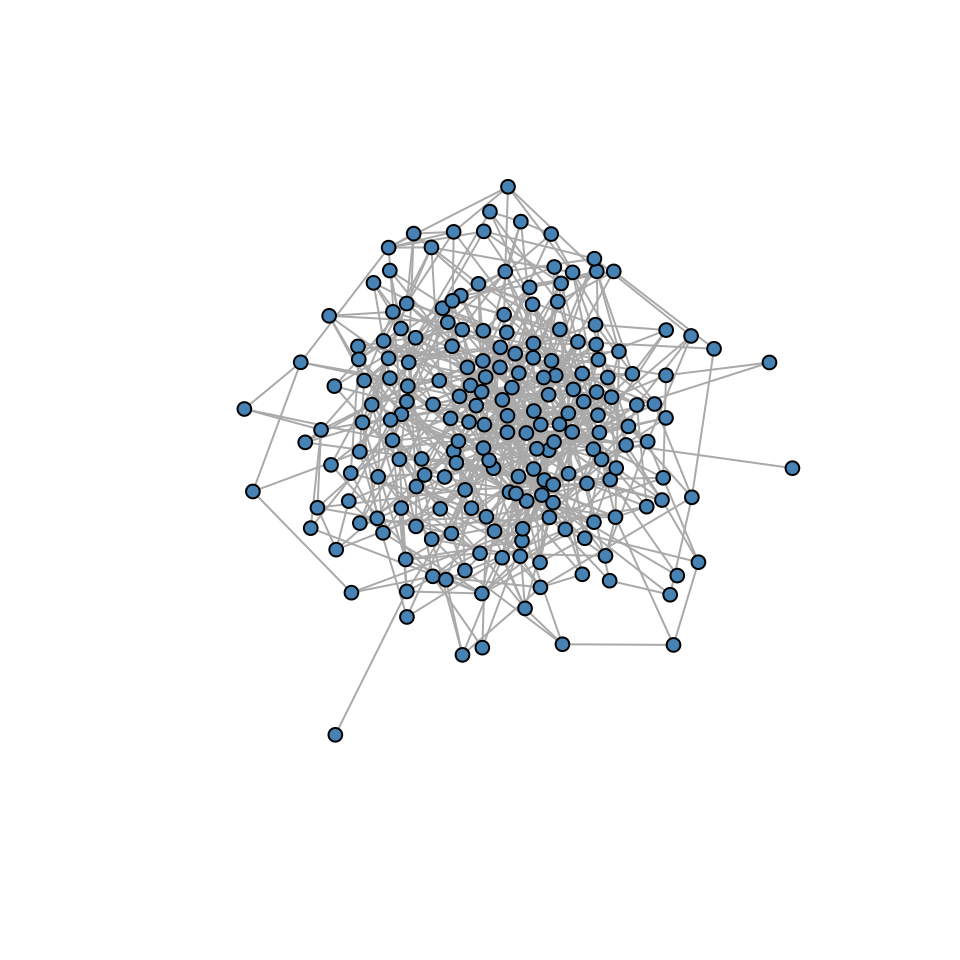
\includegraphics[width=0.5\linewidth]{phd-thesis_files/figure-latex/fig1-1} 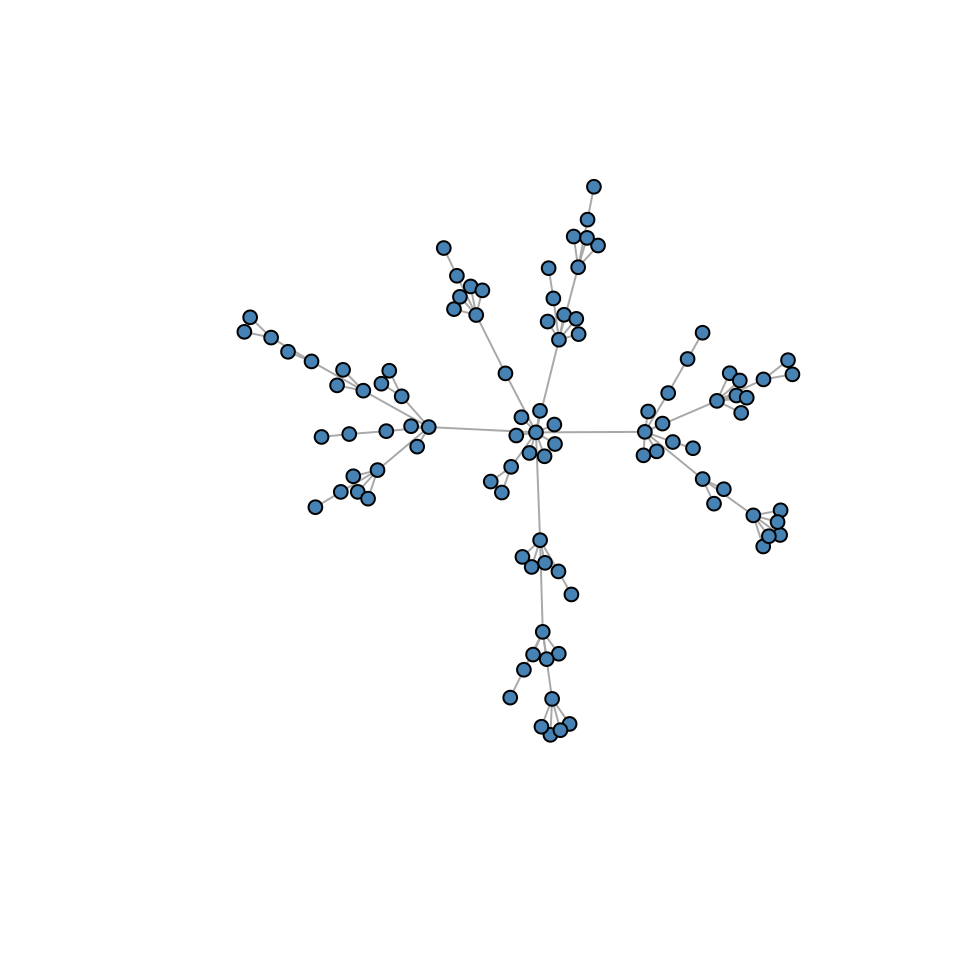
\includegraphics[width=0.5\linewidth]{phd-thesis_files/figure-latex/fig1-2} \caption{Two examples of networks, composed of dots and lines. The left network is a random graph based on the Erdős--Rényi model {[}\protect\hyperlink{ref-Erdos1960}{19}{]} and the one on the right is created using the preferential attachment principle that characterizes scale-free networks with hub nodes, such as the World Wide Web {[}\protect\hyperlink{ref-Barabasi1999}{20}{]}.}\label{fig:fig1}
\end{figure}

Since studying complex systems falls intro the domain of science's responsibilities, and graphs seem to be an intuitive way of representing such systems, the emergence of a new field called network science was inevitable {[}\protect\hyperlink{ref-Barabasi2013}{21}{]}.
Its purpose is to establish a unified set of tools and methods to study the properties of any type of network that emerges across disparate fields.
A variety of software tools for network visualization and analysis have been released throughout the years, ranging from generic-purpose {[}\protect\hyperlink{ref-Csardi2006}{22}--\protect\hyperlink{ref-Shannon2003}{25}{]}, to tools more suitable for studying biological {[}\protect\hyperlink{ref-Dahlquist2002}{26}--\protect\hyperlink{ref-Sidiropoulos2017}{29}{]} or social networks {[}\protect\hyperlink{ref-Smith2009}{30},\protect\hyperlink{ref-Kalamaras2014}{31}{]}.
The use of such tools enables the discovery of fundamental laws that characterize the function of systems represented by networks.
In addition, it allows us to study in detail the networks' systemic structure and derive key principles that drive their evolution and emergent behavior.
Anthropological research for example uses network theory to study people and their relationships, and explain emergent complex phenomena such as human behavior.
Neuroscience uses network analysis methods to detect anomalies in diseased human brains {[}\protect\hyperlink{ref-Chatterjee2021}{32}{]}.
The impact of online social networks is studied to understand and predict future personal and profit-oriented communication (online marketing) {[}\protect\hyperlink{ref-Mislove2007}{33}{]}.
Epidemiologists use graph-based methods to model the spread of diseases like COVID-19, predict the future course of outbreaks and evaluate strategies to control epidemics {[}\protect\hyperlink{ref-Maheshwari2020}{34}{]}.
Molecular biologists study intra- and intercellular signaling networks to understand the mechanisms behind biological processes and investigate the causes of network dysregulation, often leading to the emergence of particular disease phenotypes.
Such network-based approaches have significant clinical applications since they have the potential to assist in the discovery of new disease genes and modules, and the identification of drug targets and biomarkers for complex diseases {[}\protect\hyperlink{ref-Barabasi2011}{35}{]}.

The work presented in this thesis is heavily based on this network medicine paradigm, with causal molecular interaction networks as the main object of study.
Our primary focus is on protein-protein interaction (PPI) networks, with proteins as nodes and their physical contacts and interactions as links, and gene regulatory networks, represented for example by directed regulatory relationships between transcription factors and genes (TF-TG networks).
These types of networks demonstrate a system of signal transduction pathways connected by crosstalk and embedded in feedback loops, forming what is known as the \emph{Prior Knowledge Network} (PKN).
The causality property of the PKN stems from the fact that the network links are directed (i.e.~protein X affects protein Y) and signed (Y is inhibited or activated as a result).
It is exactly this causality information that allows the investigation of behaviors from a systems perspective.
Such networks form the basis for the study and computational modeling of cancer, which is another subject of investigation in this thesis.
In the subsequent chapters, we will discuss how we addressed problems related to the formalization, access and public sharing of the knowledge encoded in the PKN.

\newpage

\hypertarget{knowledge-from-a-stack-of-papers}{%
\section*{Knowledge from a stack of papers}\label{knowledge-from-a-stack-of-papers}}
\addcontentsline{toc}{section}{Knowledge from a stack of papers}

\indent

Where does the information that is used to build knowledge networks originate from?
One of the most widely adopted ways to record and share knowledge, has been the publication of scientific findings in specialized journals.
This has resulted in a major challenge that researchers in the life sciences face, which is to stay updated with the huge amount of information that is published on a daily basis (Figure \ref{fig:fig2}).
It becomes impossible for the average scientist to find, read, extract and use that information in an efficient manner without the use of databases.
Even when using databases, one is often confronted with both chronically incomplete knowledge, and also a lack of sufficient contextual information to assess when exactly the knowledge is valid.



\begin{figure}

{\centering 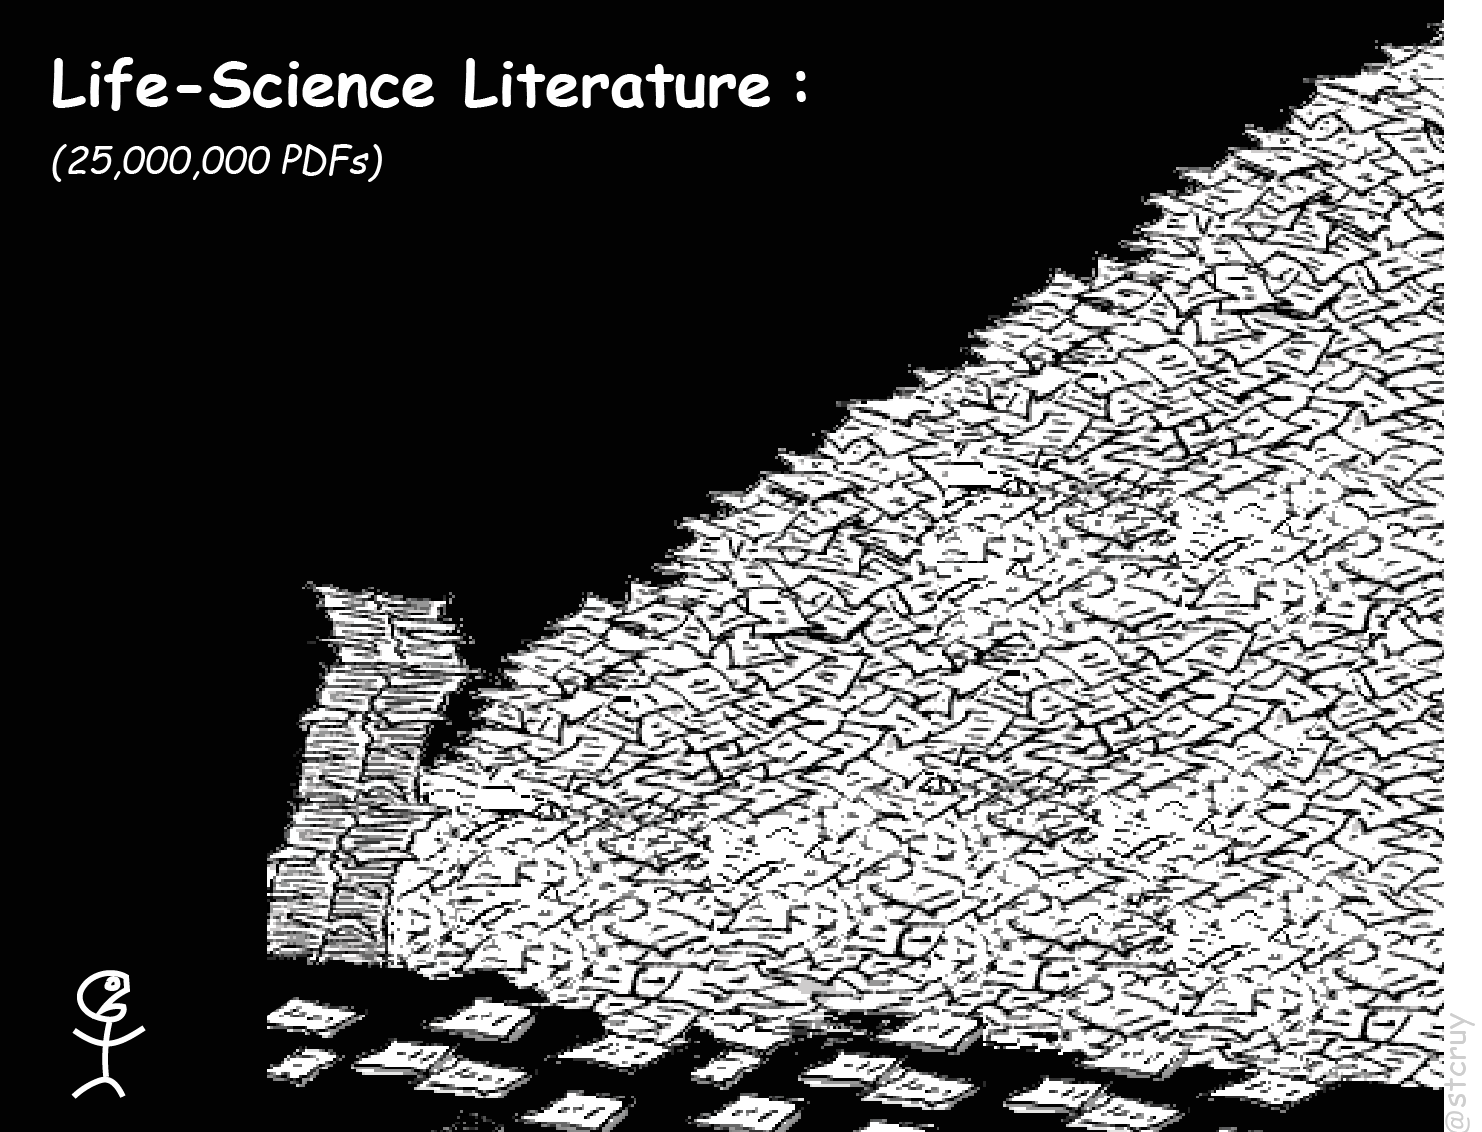
\includegraphics[width=0.75\linewidth]{img/papers} 

}

\caption{Human vs Life-Science Literature. How can humans stay up-to-date with increasing knowledge stored in PDF files? {[}\protect\hyperlink{ref-Vercruysse2019a}{36}{]}}\label{fig:fig2}
\end{figure}

A severe problem lies already at the data entry stage.
Biocurators are people whose main task is to read the scientific literature and translate knowledge into a precise, computable form, ready to be inserted into databases {[}\protect\hyperlink{ref-Howe2008}{37},\protect\hyperlink{ref-Ammari2018}{38}{]}.
The huge body of literature existing today is full of inconsistencies and inaccuracies, so expert interpretation and annotation are essential.
But current databases are limited in what they can contain, because there exists no easy way to properly transfer all kinds of complex knowledge or ideas into them, in the first place.
Moreover, the annotation tools that biocurators use are not intuitive nor flexible enough to be used by large crowds of people, to convert vast amounts of relevant knowledge from the scientific literature into the respective databases.
The insufficient funding to curate scientific results into databases, and the cost of creating a new knowledge base for every new project, are some extra confounding factors.
Because of this, researchers all over the world have to spend considerable time performing ad-hoc manual curation of publications that are relevant for their project, often with improvised approaches (Word, Excel).
At best they also spend time developing a specialized curation platform or computational methods to extract knowledge, which can only capture a fraction of the ``actual reported truth'' {[}\protect\hyperlink{ref-Jenssen2001}{39}{]}.
Nonetheless, all these efforts form a significant part of the scientific enterprise, assisting in the creation of digital knowledge repositories, which are subsequently used to build PKNs for the computational modeling of biological processes.

\vspace{15pt}

A list of tools have been created to assist biocurators in their annotation tasks.
Notably, the IntAct editor is an open-source desktop application software that enables IntAct curators and members of the IMEx consortium to annotate molecular interactions {[}\protect\hyperlink{ref-intact-editor}{40}{]}.
Because of the lack of installation instructions and documentation, coupled with a complex interface, specialized training from senior IntAct curators is required to learn how to use this software.
Nonetheless, it is one of the most used and effective tools for the job, since it has been around for a lot of years and during that time, there has always been a spirit of close collaboration between developers and curators to implement features, solve bugs and in general improve the annotation capabilities of the software.
Canto is another tool that was built to support community curation in the PomBase fission yeast database {[}\protect\hyperlink{ref-Rutherford2014}{41}{]}.
It has now expanded its original purpose to support curation of other model organism databases and different molecular data types (e.g.~annotation of a larger set of GO terms).
Canto's respective website provides extensive documentation and step-by-step user guidance throughout the annotation procedure {[}\protect\hyperlink{ref-canto-doc}{42}{]}.
A user management mechanism is incorporated in the software so as to allow proper monitoring of curation tasks and efficient communication between curators for work prioritization.
In addition, two relatively new tools have been developed for the curation and visualization of molecular interaction maps: NaviCell {[}\protect\hyperlink{ref-Kuperstein2013}{43}{]} and MINERVA {[}\protect\hyperlink{ref-Gawron2016}{44}{]}.
These tools facilitate knowledge exploration in addition to knowledge annotation, allowing for an interactive user experience (e.g.~feedback via comments), enabling content sharing, supporting well known data standards (e.g.~SBGN {[}\protect\hyperlink{ref-Novere2009}{45}{]}) and thus allowing for data interoperability and re-use.
All the aforementioned annotation tools are limited by the fact that they are not generic enough to curate any type of information, with most of them representing specialized solutions pertaining to specific annotation purposes.
Most tools require extra technical configurations and software to include additional levels of contextualized details required for current and future curation efforts.

\newpage

To obtain support from computational pipelines that will help us process vast amounts of knowledge and advance our understanding of processes in nature, we must be able to efficiently annotate and store information that is highly detailed and contextualized.
Hereby, the knowledge's inherent complexity should be kept manageable and understandable by humans and machines alike.
In order to accommodate for a much more powerful, flexible, and reusable annotation process, an intuitive curation and knowledge formalization method was developed, called VSM (Visual Syntax Method) {[}\protect\hyperlink{ref-vsm-paper}{46}{]}.
VSM enables scientists to capture any type of knowledge with any type of contextual information, in a way that is understandable by both humans and computers.

Part of the work in this thesis has been to assist in the implementation of a software module that implements VSM as a general-purpose, web-based user interface, named VSM-box {[}\protect\hyperlink{ref-vsm-box}{5}{]}.
This software component was used to build CausalBuilder, a prototype curation interface for the annotation of causal molecular interactions {[}\protect\hyperlink{ref-Toure2021}{6}{]}.
CausalBuilder uses VSM to generate concrete, customizable templates that represent causal statements.
It supports the export of the annotated statements in standard signaling formats, such as CausalTAB {[}\protect\hyperlink{ref-Perfetto2019}{7}{]}, which can be stored in relevant databases or used to build computational models of biological processes.
To support the large variety of contextual information related to causal molecular interactions between biological entities, allowing for a finer disambiguation between seemingly similar or conflicting causality statements (e.g.~a transcription factor simultaneously up and down regulating a target gene in different cellular contexts), CausalBuilder was designed to comply with a list of guidelines (MI2CAST) that were developed exactly for this purpose {[}\protect\hyperlink{ref-Toure2020}{47}{]}.
All in all, CausalBuilder provides biologists and curators with a simple user interface for the annotation of causal regulatory knowledge, translating highly contextual information about molecular interactions from scientific publications to a computable form.

\newpage

\hypertarget{biological-dictionaries-aid-in-the-curation-of-complex-knowledge}{%
\section*{Biological Dictionaries aid in the curation of complex knowledge}\label{biological-dictionaries-aid-in-the-curation-of-complex-knowledge}}
\addcontentsline{toc}{section}{Biological Dictionaries aid in the curation of complex knowledge}

\indent

During the design process of the VSM-box tool and its application, CausalBuilder, we came across a critical technical issue that needed to be addressed, and whose resolution had ramifications outside of the intended scope of our work.
Due to the high degree of complexity within the domain of biology, biocurators need to annotate diverse information, taken from a plethora of biological resources and vocabularies.
To enable a wider expressiveness in the annotation of causal statements, the recommended list of ontologies and vocabularies of the MI2CAST standard had to be rather extensive {[}\protect\hyperlink{ref-mi2cast-doc}{48}{]}.
Since CausalBuilder conforms to the MI2CAST standard, a unified way to retrieve, format and display vocabulary terms from different databases was needed.
We illustrate this with an example: in Figure \ref{fig:fig3}, a simple VSM-template that a curator can use to annotate a causal statement with CausalBuilder is shown.
Following the MI2CAST guidelines, the source entity of the causal statement (first box in Figure \ref{fig:fig3}) must always be specified and a list of recommended resources where the annotation could potentially originate from is provided {[}\protect\hyperlink{ref-mi2cast-doc}{48}{]}.
We limit the number of these resources to three in this example, making it so that the source biological entity can be annotated as a protein (from UniProt {[}\protect\hyperlink{ref-TheUniProtConsortium2019}{49}{]}), a complex (from Complex Portal {[}\protect\hyperlink{ref-Meldal2019}{50}{]}), or an RNA transcript (from RNAcentral {[}\protect\hyperlink{ref-RNACentral2018}{51}{]}).
The intended use case is that the curator will type in a string (e.g.~``tp53'') and a list of terms and descriptive metadata from the three respective standard databases will be returned.
This information can be displayed by VSM-box in an autocomplete drop-down menu to ease the selection of the appropriate term by the curator.



\begin{figure}
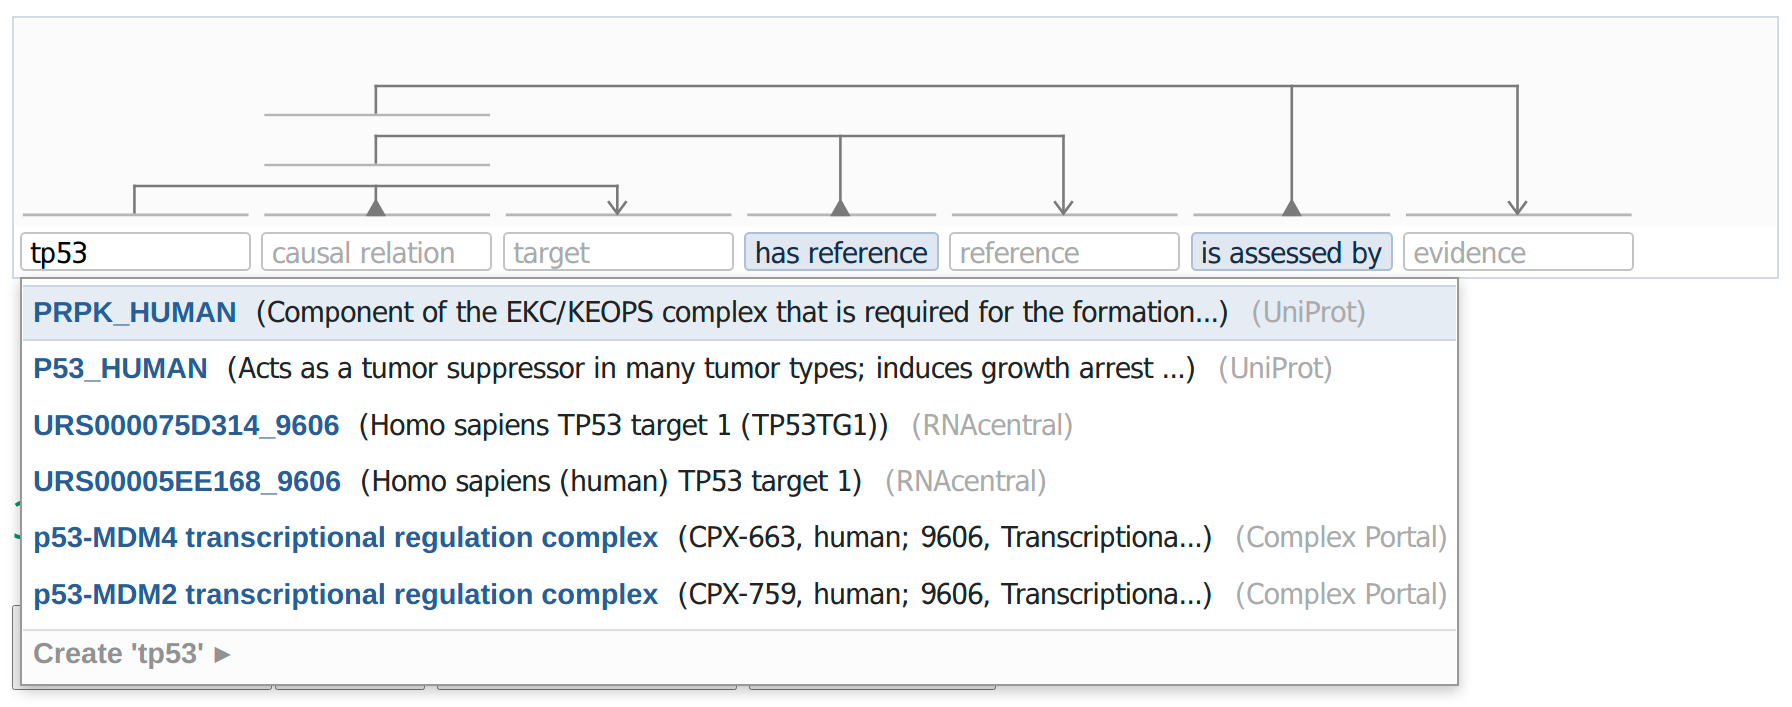
\includegraphics[width=1\linewidth]{img/causalBuilder_screenshot} \caption{Querying multiple data resources using the VSM-box technology in CausalBuilder. The user enters a string of interest and selects a list of resource types (not shown here) for the source entity, following the MI2CAST curation guidelines. The UBDs stand as a hidden translator between the query launched from the curator interface and the respective database data, returning a list of uniformly-structured matches, shown as a drop-down list to the user. The matches consist of a curator-friendly main term (shown in blue) and metadata like identifier, name of species, textual description, resource name etc., that a user can use to disambiguate between the different concepts.}\label{fig:fig3}
\end{figure}

\newpage

We can now clearly state the heart of the problem: the resources that offer protein, RNA and multiprotein complex data, have different online APIs to serve their information, and it is usually structured in diverse formats.
Therefore, it was necessary to design a generic solution that would translate all the necessary information from the recommended resources of the MI2CAST standard into a unified representation schema.
Then, we could implement modules that ``talk'' to the databases and translate the provided information into this uniform data format.
As a result of having a standardized way to represent data from various disparate resources, VSM-box and other curation tools could easily process the returned data load and create drop-down menus to help users in their annotation tasks (as shown in Figure \ref{fig:fig3}).
The outcome of all this effort was the implementation of UBDs (Unified Biological Dictionaries, see \textbf{\protect\hyperlink{Paper1}{Paper 1}}).
The reason for the name \emph{dictionaries} originates from the abstract data type called \emph{associative array} (also known as \emph{map} or \emph{dictionary}), which is a collection of (\emph{key, value}) pairs, and is an integrated feature of many programming languages.
For our application, we reasoned that the minimum information that is needed for the unique identification of concepts for curation tasks is a computer-friendly ID and a human-friendly term, precisely matching the \emph{key} and \emph{value} of the associative array's data structure.

An unforeseen consequence of the UBDs implementation was that by covering most of the vocabularies and ontologies recommended by the MI2CAST standard, we ended up mapping into a unified format a large amount of diverse terminologies across life sciences.
This happened because our solution encapsulated and extended other similar efforts, such as the BioPortal {[}\protect\hyperlink{ref-Whetzel2011}{52}{]} and EBI Search {[}\protect\hyperlink{ref-Madeira2019}{53}{]} web services.
We therefore managed to bring even more biomedical ontologies and biological data resources under one umbrella, and subsequently increase the accessibility, interoperability and reusability of the provided data {[}\protect\hyperlink{ref-Wilkinson2016}{54}{]}.
So, even though UBDs main user is the software engineer building curation tools (as we were at the beginning of this effort with CausalBuilder), several computational researchers can benefit from our implementation, if they need to query disparate biological resources for lightweight information (i.e.~terms, identifiers and some metadata) using a single programmatic interface.
In the end, the feedback we got from biocurators who tested the CausalBuilder tool was very encouraging, pointing out that we had proceeded in the right direction with our efforts to build UBDs, the hidden machinery enabling all the autocomplete ``magic'' to happen in VSM-box's user interface.

The implementation of UBDs put us in a position to confront problems that biocurators face during their annotation tasks, which haven't yet been properly addressed by any existing technology.
One of these challenges is that biocurators often need to annotate terms in a specific domain or novel field, for which there is still no authoritative database or ontology nor a community consensus about the respective terminology {[}\protect\hyperlink{ref-Hartmann2019}{55}{]}.
A similar challenge manifests when new knowledge is discovered or similarly, further contextual information related to existing knowledge comes into light, as a result of scientists' constant drive for progress.
This eventually leads to the constant refactoring of ontologies and identifiers, subsequently making biocurators life even more difficult.
To respond to these challenges, biocurators create project-specific, \emph{ad-hoc} vocabularies that are not openly accessible and usually become obsolete after some time passes.
We reasoned that with the UBDs infrastructure in place, we could do better.

In summary, the core of the problem is two-fold: first, biocurators need a simple way to annotate new information that does not yet exist in any resource and second, this information needs to be shared publicly for further review and management by expert communities.
To tackle this problem, we collaborated with experts from PubDictionaries, an online repository of publicly accessible and editable dictionaries {[}\protect\hyperlink{ref-Kim2019}{56}{]}.
Using the online interface of PubDictionaries, curators can create simple dictionaries, consisting of terms and identifiers of their own choice, solving the second part of the problem.
Additionally, by updating the PubDictionaries API and connecting all existing and future public dictionaries with UBDs and their underlying unified format, we streamlined their use in annotation tools and solved the first part of the problem.
The technical work was carried out during an intense hacking week at the ELIXIR Biohackathon 2021 event and the implementation details are described in \textbf{\protect\hyperlink{Paper2}{Paper 2}} of this thesis.
As a final result, we showcased a demo in which curators could use their public, ad-hoc terminologies from PubDictionaries, to annotate a simple sentence using the VSM-box interface.

\newpage

\hypertarget{psicquic-chapter}{%
\section*{Sharing causal interactions with PSICQUIC}\label{psicquic-chapter}}
\addcontentsline{toc}{section}{Sharing causal interactions with PSICQUIC}

\indent

Defining standards is a very important initiative across scientific disciplines, since it facilitates the accessibility and sharing of information amongst data users as well as the interoperability of software tools that produce or process the respective data, thereby increasing the quality of research findings {[}\protect\hyperlink{ref-Wilkinson2016}{54}{]}.
Following this logic, after the curation of causal molecular interactions from scientific literature has been achieved, the next step is to store this information to a standard data format.
One of the most detailed, community-standard formats for representing molecular interaction data is the PSI molecular interaction (MI) XML format, released by the Human Proteome Organization Proteomics Standards Initiative (HUPO-PSI) {[}\protect\hyperlink{ref-Hermjakob2004}{57}{]}.
The newest version of this standard is the PSI-MI XML 3.0 {[}\protect\hyperlink{ref-Sivade2018}{58}{]}.
A simplified format for interaction data was provided by the same organization, called the Molecular Interaction Tabular format (PSI-MITAB).
PSI-MITAB has become popular amongst the scientific community since it is more user-friendly and Microsoft Excel-compatible, compared to the respective XML-based format {[}\protect\hyperlink{ref-Kerrien2007}{59}{]}.
PSI-MITAB version 2.7 in particular, encapsulated many details of interest regarding a molecular interaction in a total of 42 columns, but it did not include information about its causality.
This resulted in an effort to standardize the signaling information and subsequent vocabulary terminology for causal molecular interactions, originally led by SIGNOR's database curators {[}\protect\hyperlink{ref-Licata2019}{60}{]}.
The new PSI-MITAB version 2.8 (also called \textbf{CausalTAB}), included four new columns to incorporate additional details related to a molecular interaction's directionality (defining the biological roles of the regulator and target, one column each), regulatory mechanism (e.g.~indirect causal regulation or post-translational modification) and resulting effect (up or down regulation of the target) {[}\protect\hyperlink{ref-Perfetto2019}{7}{]}.

After having a signaling data format for molecular interactions in place, the next challenge was to find a way to share such information efficiently.
The heart of the problem was the same even without the addition of causality information: a large number of molecular interaction databases exist, each one with different APIs to access the respective data.
Since no single database can incorporate the totality of molecular interactions pertaining to a specific biological system of interest, users have to collect data from diverse databases by launching queries in different websites or by directly downloading the respective files, which might not always be offered in standardized formats.
To ease the computational access and retrieval of molecular interaction data from various resources, a web service with a common query interface (PSICQUIC) and language (MIQL) was developed {[}\protect\hyperlink{ref-Aranda2011}{61}{]}.
Using the PSICQUIC web service, users can now download all relevant data files from their databases of interest in different PSI-MI compliant formats, suitable for further analysis (Figure \ref{fig:fig4}).



\newpage

\begin{figure}
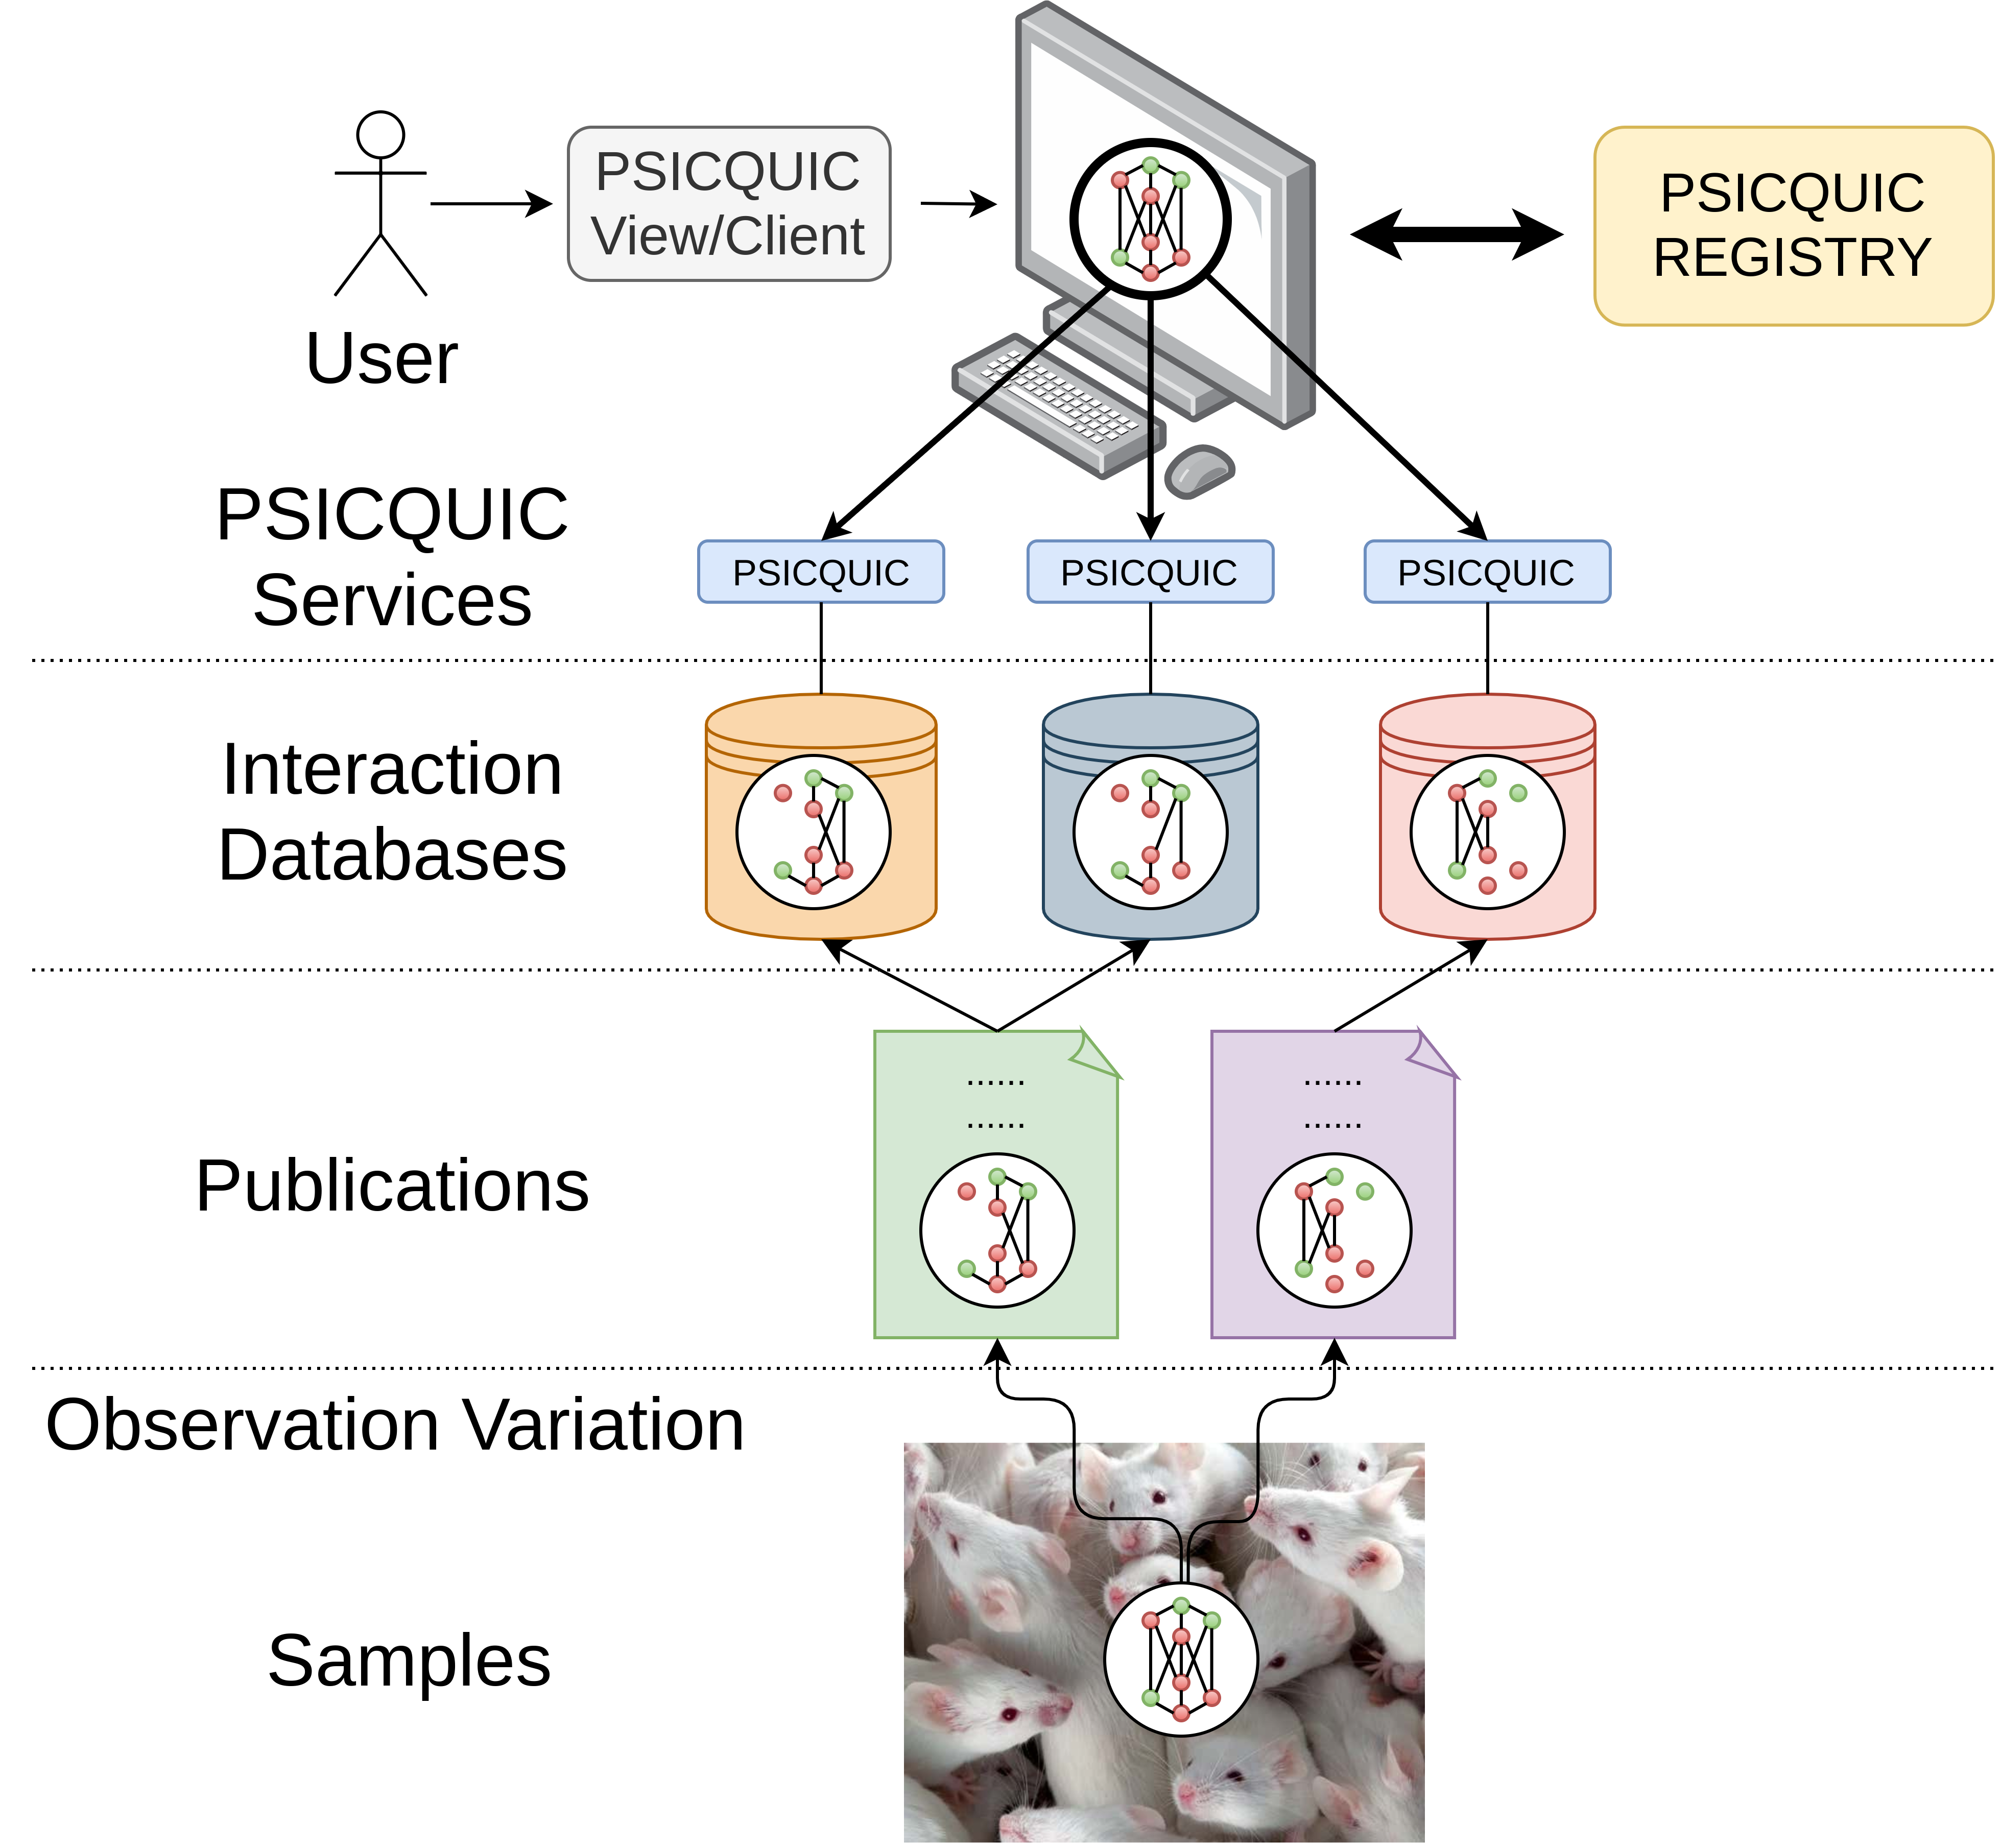
\includegraphics[width=0.9\linewidth]{img/psicquic} \caption{PSICQUIC architecture. Molecular interaction knowledge about a biological system, supported by different experimental methods, is being reported in publications. Each of these publications reports part of the actual truth about the studied system. This knowledge is curated from the respective publications and inserted to diverse molecular interaction databases. The databases share their data in standard formats (e.g.~PSI-MITAB) via the PSICQUIC web service and are part of a registry list. Users launch queries via a PSICQUIC web client to retrieve the distributed molecular interaction data and synthesize the complete observed knowledge of the studied system, suitable for further analysis and visualization.}\label{fig:fig4}
\end{figure}

With a new signaling data format established by the relevant scientific community and the PSICQUIC web service contributing to the accessibility of molecular interaction data, the next step was to support the PSI-MITAB 2.8 format in PSICQUIC.
A software project to extend the PSICQUIC platform and include causality information of molecular interactions was thus formed.\footnote{This project was funded by the GREEKC (Gene Regulation Ensemble Effort for the Knowledge Commons) COST action (\url{https://www.greekc.org/}) and was realized as a Short Term Scientific Mission (STSM) in cooperation with engineers from the IntAct team at the European Bioinformatics Institute (EBI).}
Our contribution to this effort was the development of the underlying PSICQUIC software (version 1.4) that indexes CausalTAB files provided by the respective data providers, enabling the query and subsequent download of causality-enriched interactions.
The PSICQUIC View website source code was updated to show the four new columns in the HTML table results.
Additionally, several clients that enable programmatic access to the distributed signaling data (written in Java, Python and Perl programming languages), were refactored to comply with data fitting the new standard format.
Lastly, the relevant PSICQUIC documentation was improved and reformatted to enhance user readability {[}\protect\hyperlink{ref-mitab28-doc}{62}{]}.

The aforementioned development effort spurred a series of actions that led to several improvements in the PSICQUIC platform.
The Molecular Interactions Community, is an open source community providing tools, standard formats, ontologies and modules for manipulating molecular interaction data {[}\protect\hyperlink{ref-mi-github}{63}{]}.
For example, some of these modules are used to read and write PSI-MITAB files across different versions.
Since these modules had not been updated for years (showing signs of software rot {[}\protect\hyperlink{ref-soft-rot-wiki}{64}{]}), we had to refactor the codebase and add tests to ensure its future reliability and quality.
In the end, even though we managed to complete the task and support CausalTAB in PSICQUIC via updating these modules, the need to replace them with a newer library was imminent.
JAMI is such a library, integrating all standard molecular interaction data formats such as the PSI-MI XML and PSI-MITAB, into a unified implementation, hiding the complex details of each format from the developers and thereby making their work easier {[}\protect\hyperlink{ref-Sivade2018a}{65}{]}.
The implementation work was initiated in a GREEKC workshop {[}\protect\hyperlink{ref-Hinxton2018}{66}{]} and continued during the first ELIXIR BioHackathon in Paris {[}\protect\hyperlink{ref-biohack2018}{67}{]}.
Upon finishing the support for CausalTAB in JAMI,\footnote{During the GREEKC Marseille Hackathon 2019 event, see more info on the project here: \url{https://github.com/GREEKC/hackathon-marseille/tree/master/project_descriptions/causal_psicquic}} we provided the first PSICQUIC service indexing SIGNOR's CausalTAB data at the time, made available through a development server {[}\protect\hyperlink{ref-psicquic-causalTAB-dataset}{68}{]}.

During the ELIXIR BioHackathon, the architecture details of a new cloud-based, distributed PSICQUIC service were discussed and documented for future development efforts.
The goal is to enable the data providers to upload their molecular interaction data in a fully automated process and add support for data validation.
This service will minimize the long-term commitment and maintenance from the data providers, which they cannot always afford (e.g.~deployment of the server hosting PSICQUIC).
Another outcome of the BioHackathon was the draft implementation of a new PSICQUIC View interface, aiming to modernize and update the current web application used to access PSICQUIC {[}\protect\hyperlink{ref-psicquic-view}{69}{]}.
Further work needs to be done to import and use newer technologies in the interface, which will result in better filtering and sorting of the HTML table results and more interactive, graph-based visualizations of the PSICQUIC data.
To broadly facilitate the sharing of causal interaction data, additional development efforts are needed, in particular towards improving existing PSICQUIC clients.
One such example is the PSICQUIC Universal Client, a Cytoscape app for querying multiple PSICQUIC-compliant interaction data services from a simple user interface {[}\protect\hyperlink{ref-PSICQUICUniversalClient}{70}{]}.
This client has been used in tutorials to guide novice users in the visualization and analysis of molecular interaction networks {[}\protect\hyperlink{ref-Millan2013}{71}{]}.
Lastly, two more clients that need to be updated to support the latest CausalTAB signaling format are the PSICQUIC {[}\protect\hyperlink{ref-Shannon2020}{72}{]} and PItools \texttt{R} packages {[}\protect\hyperlink{ref-Kleshchevnikov2021}{73}{]}.
These packages enable the translation of molecular interaction data directly into formats suitable for computational analysis with \texttt{R}, and therefore are crucial for relevant computational tasks.

\newpage

\hypertarget{biological-modeling-a-prelude}{%
\section*{Biological modeling: a Prelude}\label{biological-modeling-a-prelude}}
\addcontentsline{toc}{section}{Biological modeling: a Prelude}

\indent

In previous chapters we summarized our efforts related to the curation, access and sharing of causal molecular interactions, the building block of PKNs.
This is only the first step in the process of creating computational models of biological systems {[}\protect\hyperlink{ref-Wang2012}{74}{]}.
To translate signaling networks to a computational form for simulation purposes, the next step is to define the regulatory \emph{rules} (\emph{parameterization}) of the underlying system: how do the different network entities influence each other across time and potentially space, and how does the systemic behavior change when specific rules or parameters of the model are modified? {[}\protect\hyperlink{ref-Aldridge2006}{75}{]}
The formulation of the rules in mathematical terms (i.e.~they are in most cases expressed as equations), defines the mechanistic details of the studied models and thus enables the study of their dynamics.
Practically, this means that models can be used for various forms of analyses and simulations, and their outputs further investigated.
For example, models can be validated and tested for agreement with experimental observations, can make predictions and generate new hypotheses leading to the design of new experiments, and they can be subjected to various perturbations, with their subsequent effects on the studied systems quantified and thoroughly analyzed.
In addition to biological analysis, one of the more important aspects of mathematical modeling is that it enables the investigation of the underlying mechanisms that result in the manifestation of the described system's behavior.
In other words, computational models are explainable and interpretable, enabling us to answer why things happen the way they do, which is one of the driving forces behind science itself.

Several mathematical methodologies have been used to study biological systems, such as stochastic modeling, ordinary and partial differential equations (ODE and PDE modeling), Petri nets, logical modeling, Bayesian networks, cellular automata and agent-based modeling {[}\protect\hyperlink{ref-ElKalaawy2015}{76}{]}.
Each modeling paradigm encapsulates a different way of formalizing the underlying rules and makes different assumptions about the studied system.
Such assumptions can for example include the temporal and spatial properties of the modeled system (space and time can each be treated in a continuous manner or with varying degrees of discretization), the molecular scale (focus on modeling individual molecules or discrete amounts of each molecule or just considering their molar concentrations) and the nature of interactions between the molecules (reaction processes can be described as happening in a stochastic or deterministic manner).
In general, there is a trade-off between the complexity of the system that a model is constructed to simulate and the mechanistic detail incorporated in the model itself {[}\protect\hyperlink{ref-Aldridge2006}{75}{]}.
Ideally we would like to have models which can simulate highly complex systems in as much detail as possible.
This poses a significant challenge, since a more detailed representation of a biological system requires a higher level of granularity inherent in a model's formalization.
This means that more parameters are required to specify and calibrate the model for the simulation and accurate representation of reality, and larger amounts of experimental data and computational resources are also necessary.
On the other hand, by sacrificing the complexity of the studied system and making simpler models, we face overwhelming uncertainties that need to be properly quantified and integrated in any interpretation of results from such a model {[}\protect\hyperlink{ref-Groen2021}{77}{]}.
In the end, the modeling scope is a crucial factor for the choice of the appropriate methodology, and thus sufficient knowledge of the advantages and disadvantages of each formalism can be beneficial towards selecting the approach deemed most suitable for the realization of the modeling objectives.

In this thesis we focus on Boolean modeling, one of the simplest formalizations for the modeling of complex biological systems {[}\protect\hyperlink{ref-Schwab2020}{78}{]}.
In this type of qualitative approach, every individual entity has a binary state denoting activity (1) or inactivity (0) and time is discretized {[}\protect\hyperlink{ref-Kauffman1969}{79}{]}.
Every interaction that affects a target entity is assembled into a Boolean equation which defines that particular target's output activity in the next time step.
To formulate such a Boolean equation, only knowledge of the regulatory network topology is needed, along with the use of logical operators that describe how the combined activity of the regulators affects the target.
This inherent simplicity in defining the rules is what makes the Boolean formalism attractive to modelers.
Moreover, since the PKN is one of the core elements that characterize the Boolean rules, this explains why we spent a large amount of our efforts in this thesis to make sure modelers get the proper contextual prior knowledge.
Lastly, another advantage of Boolean modeling is that it does not require the specification of parameters such as kinetic rate constants and initial concentrations that are a strong prerequisite in other modeling formalisms (e.g.~in ODE modeling), where there is always a need for large and expensive amounts of data that might be either lacking or not enough to adequately characterize the rules.

Continuing with the explanation of the modeling formalism, a logical model is a list of mathematical equations expressed in Boolean algebra.
The state of such a system is represented by a series of 0's and 1's, each corresponding to the activity state of a signaling entity.
Using the Boolean rules, we can update the system's state by deciding on the order that each of its equations are applied, to derive the next entity states.
Therefore, a synchronous update scheme can be defined as calculating the output of all Boolean equations of the model at the same time.
In contrast, randomly specifying one or more equations to update can result in various forms of asynchronous dynamics, which enable the inclusion of processes with different time scales in a logical model.
By repeatedly applying the Boolean rules, systemic states that either do not change (\emph{fixpoints}) or ones that demonstrate cycling patterns, can be reached.
These are the \emph{attractors}, which represent solutions to the system of equations that constitute a Boolean model and their identification is synonymous to the study of the long-term dynamical behavior of the modeled system.
Attractors have been shown to be biologically meaningful, either by representing specific phenotypic outputs {[}\protect\hyperlink{ref-Kauffman1993}{80}{]} or transitions between system states like in the cell cycle {[}\protect\hyperlink{ref-Faure2006}{81}{]}.

\newpage

Several computational tools have been developed to aid in the dynamical analysis of Boolean models {[}\protect\hyperlink{ref-Abou-Jaoude2016}{82}{]}.
These tools enable users to easily create and edit logical models, identify different types of attractors and their reachability properties, analyze model state evolution over time, investigate phenotypic outputs subject to various types of perturbations, explore different model parameterizations and calibrate models to fit experimental data, among others {[}\protect\hyperlink{ref-Naldi2018a}{83}{]}.
The existence of such a plethora of tools has enabled the modeling of complex diseases, the discovery of potential therapeutic solutions and the investigation of biomarkers that correlate with patients' response to specific pharmaceutical drugs.
In particular, the derivation of mechanistic insights related to the manifestation of diseases, is one of the main challenges that computational modeling efforts strive to address towards achieving the goal of personalized medicine {[}\protect\hyperlink{ref-Hood2011}{84}{]}.
In light of this, several logical modeling approaches have been used to stratify patients based on the integration of multi-omics data {[}\protect\hyperlink{ref-Beal2018}{85}{]}, build patient-specific models that aid in the understanding of drug sensitivity and cancer resistance mechanisms {[}\protect\hyperlink{ref-Eduati2017}{86}--\protect\hyperlink{ref-Tognetti2021}{88}{]} and help identify novel therapeutic targets {[}\protect\hyperlink{ref-Saadatpour2011}{89}--\protect\hyperlink{ref-Eduati2020}{91}{]}.
Part of the work in this thesis has been to complement the aforementioned approaches by developing a software pipeline that uses causal prior knowledge and tailors Boolean models to cell-specific cancer signaling activities (\textbf{\protect\hyperlink{Paper3}{Paper 3}}).
These models can subsequently be used to predict combinatorial treatments that aid in the prioritization of drugs in high-throughput screening technologies and will eventually provide better clinical decision support for cancer patients, helping us find optimal drug-patient matches.

\newpage

\hypertarget{clean-code}{%
\section*{Clean Code}\label{clean-code}}
\addcontentsline{toc}{section}{Clean Code}

\indent

Our main goal is to use causal molecular knowledge and signaling activity data to build and parameterize Boolean models to represent specific cancer cell systems, and study their behavior in the presence of in-silico drug perturbations.
As such, the importance of the underlying scientific software that enables these computational tasks is unquestionable.
Such software needs to satisfy a list of requirements pertaining to its suitability for practical use {[}\protect\hyperlink{ref-Wilson2014}{92}{]}.
Such practices ensure that the software does what it is intended to do and its produced scientific simulations can be used to inform decision-making for clinical applications.
In other words, for the scientific results of the simulations to be \emph{actionable} and \emph{trustworthy} {[}\protect\hyperlink{ref-Coveney2021}{93}{]}, the following software requirements are not just optional, but rather a necessity.
At first, challenges related to automation, efficiency and optimization in terms of the computational resources necessary to perform the simulations and analyses, need to be properly addressed.
To promote collaboration and allow others to study, use and further develop the software, the respective codebase needs to be open sourced {[}\protect\hyperlink{ref-Barnes2010}{94},\protect\hyperlink{ref-Prlic2012}{95}{]}.
Standard formats for input and output should be supported, as well as standard libraries for common programming tasks, enabling the effortless integration with related software.
Also, sufficient documentation needs to be provided, containing installation guidelines and explanations for the various configurations used in the simulations {[}\protect\hyperlink{ref-Karimzadeh2018}{96}{]}.
Simple examples of use and related tutorials should be part of such documentation as well {[}\protect\hyperlink{ref-List2017}{97}{]}.
The usability of the software can also be increased by applying better programming architecture and design principles (e.g.~writing modular code), which also makes the software easier to test, extend and verify.
Making the results of the simulations verifiable (i.e.~by ensuring that the algorithmic procedures and the model equations are correctly coded),\footnote{Read more on verification \protect\hyperlink{gtrr}{here}} will increase their reproducibility, further supporting the aforementioned goals {[}\protect\hyperlink{ref-Sandve2013}{98}{]}.
All in all, there can only be gains if the code is \emph{clean} and properly taken care of {[}\protect\hyperlink{ref-Martin2009}{99}{]}.

In Figure \ref{fig:fig5} we present an overview diagram of the DrugLogics software pipeline.
This pipeline represents a computational software system aiming to assist in the identification of synergistic drug combinations.
The pipeline's two main modules, Gitsbe (Generic Interactions To Specific Boolean Equations) and Drabme (Drug Response Analysis to Boolean Model Ensembles), are both written in Java.
Gitsbe, using as input a PKN and a signaling activity profile for some of the key entities in the input network, creates Boolean models based on a genetic algorithm approach and calibrates them to best fit the training signaling activity data.
Boolean models with higher fitness have fixpoint attractors whose node states better match the binary signaling activities.
Calibration refers to changes in the Boolean equations to produce such high fitness models.
These changes can simply be variations in the parameterization such as mutations in the Boolean rules (e.g.~a logical OR becomes a logical AND and vice-versa) or topological changes, such as the addition or removal of a regulator's effect on a particular target.
Thus the Boolean models in Gitsbe's produced ensemble are parameterized differently, but are all essentially approximate representations of the same biological system.
These variant Boolean models are then used as input to Drabme, to test the effect of several perturbations from a given drug panel and quantify their combinatorial interaction patterns using well-known synergy frameworks (namely HSA {[}\protect\hyperlink{ref-gaddum1940pharmacology}{100}{]} and Bliss {[}\protect\hyperlink{ref-Bliss1939}{101}{]}).
Leveraging the wisdom of the crowds {[}\protect\hyperlink{ref-Galton1907}{102},\protect\hyperlink{ref-Marbach2012}{103}{]} using Gitsbe's models, Drabme's output predictions contribute in reducing the exponentially large drug space that is associated with combinatorial treatments for the targeted therapy of cancer, providing a list of candidate combinations to test in the lab, before a viable solution is found for a patient.



\begin{figure}
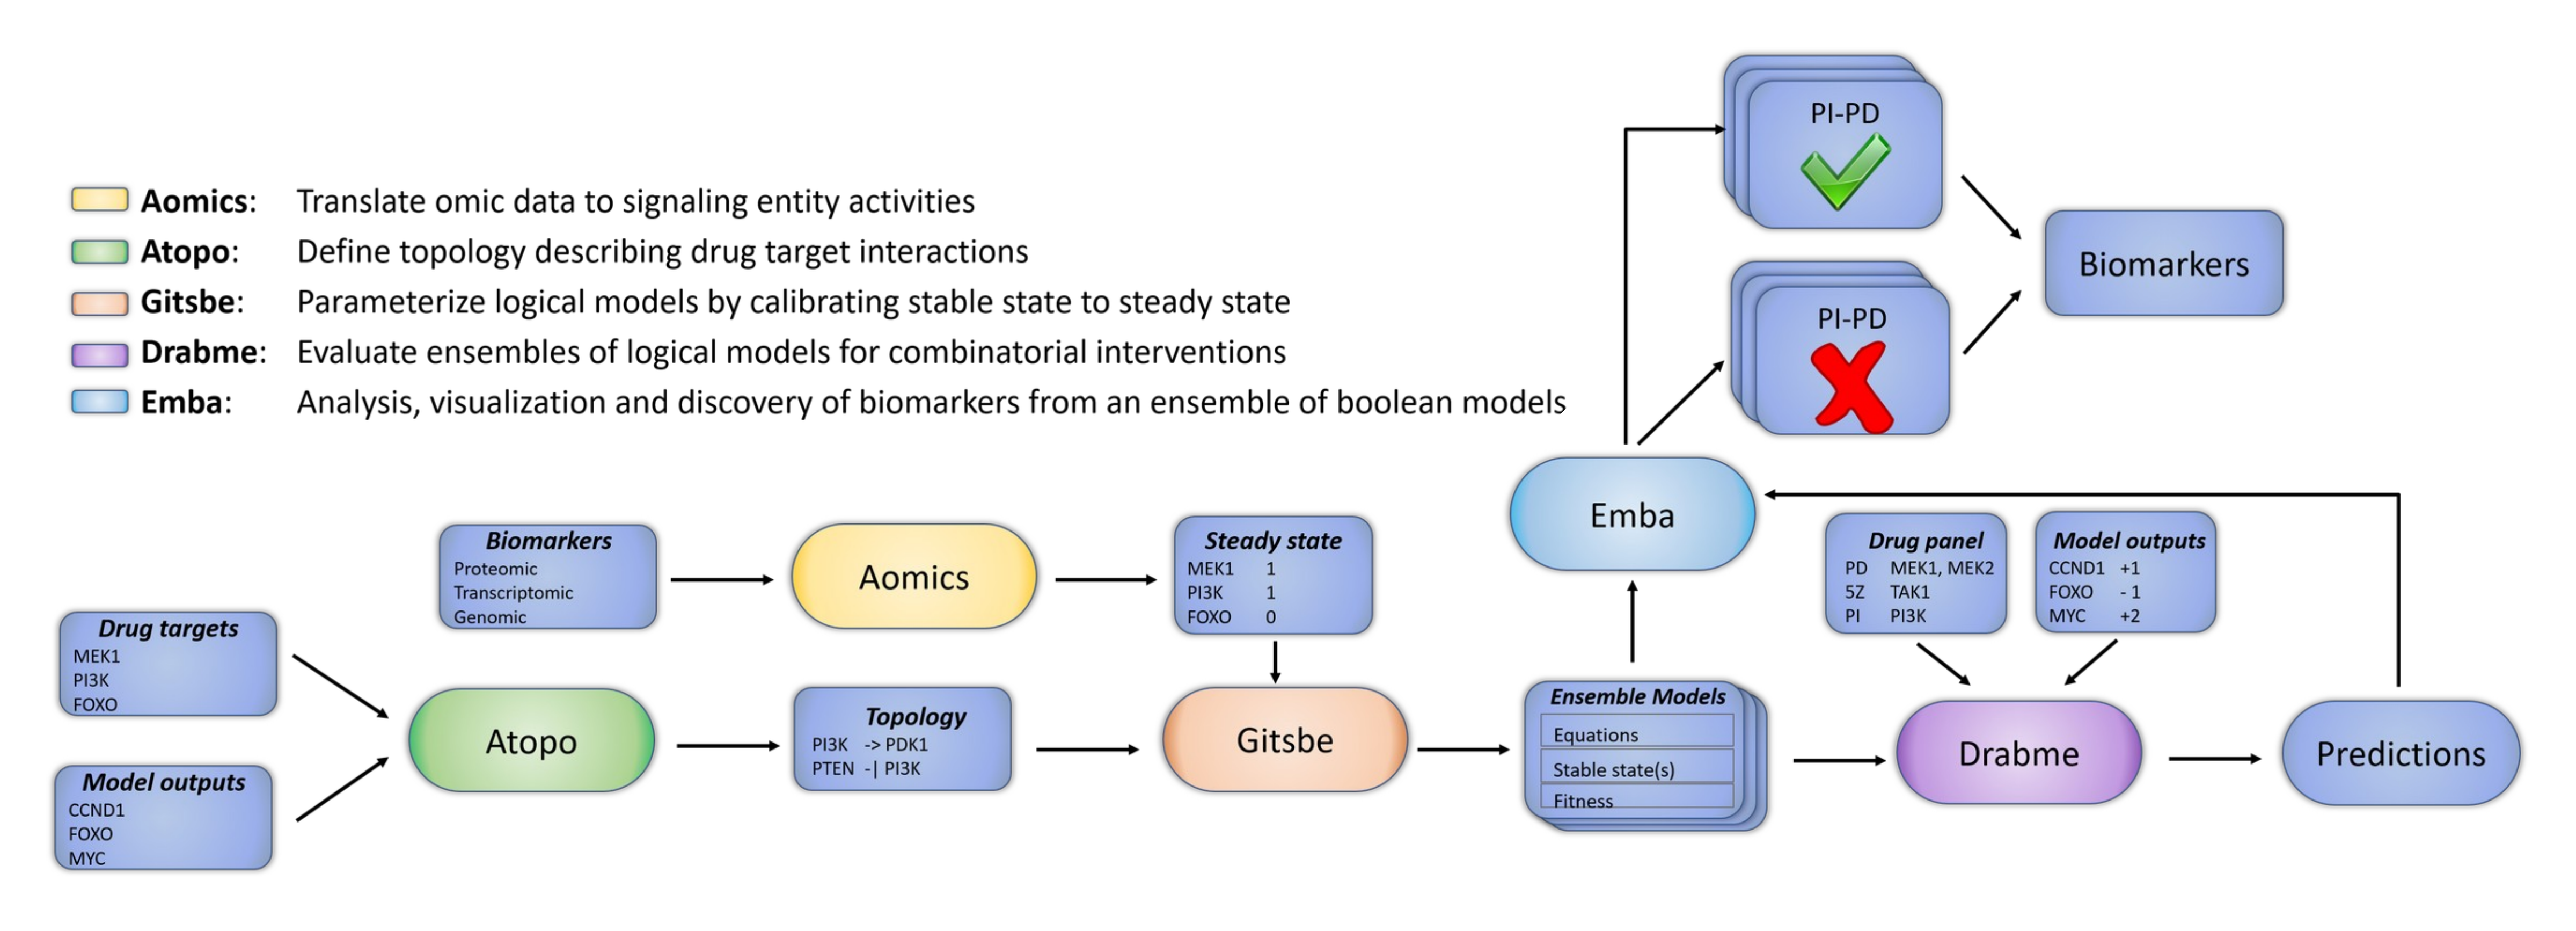
\includegraphics[width=1\linewidth]{img/pipeline} \caption{The DrugLogics software pipeline. A series of connected modules that build a regulatory topology incorporating specific drug targets, parameterize Boolean models to a specific cancer signaling profile assembled from various omics data and simulate drug combination perturbations. The output models and their predictions can be further analyzed to explain the difference between phenotypes and thus identify biomarkers that make a particular drug combination synergistic.}\label{fig:fig5}
\end{figure}

The development of Drabme and Gitsbe was part of the latest stages of a previous research thesis and it was mostly exploratory work {[}\protect\hyperlink{ref-Flobak2016}{104}{]}.
To lay the groundwork for the analyses and investigations of the papers included in this thesis, additional software development needed to be done.
We started by refactoring the source code to increase its readability, maintainability and extensibility.
Java classes were restructured, variables and functions were renamed to reflect current best programming practices, code written from scratch for common tasks such as string manipulation was replaced with reusable Java components (e.g.~using libraries from Apache Commons {[}\protect\hyperlink{ref-ApacheCommons}{105}{]}) and the Maven project management tool {[}\protect\hyperlink{ref-Maven}{106}{]} was used to enable easier source compilation, installation and packaging (all the Java code was bundled in a single compressed file for ease of use).
To increase interoperability of our software, we used the Java library BioLQM {[}\protect\hyperlink{ref-Naldi2018}{107}{]} to enable the export of the produced Gitsbe models to standardized formats in the logical modeling community, such as GINML (used in GINsim, a software tool enabling the definition, analysis and simulation of regulatory graphs based on the logical formalism {[}\protect\hyperlink{ref-Naldi2018b}{108}{]}), SBML-qual (a standard designed for the representation of multivalued qualitative models of biological networks {[}\protect\hyperlink{ref-Chaouiya2013}{109}{]}) and BoolNet (file format of the models built with the BoolNet \texttt{R} package, used for the simulation and analysis of Boolean networks {[}\protect\hyperlink{ref-Mussel2010}{110}{]}).
For the calculation of fixpoint attractors, an external scripting-based tool was used by default {[}\protect\hyperlink{ref-Veliz-Cuba2014}{111}{]}.
We added a built-in, integrated Java solution using BioLQM, which apart from fixpoints can also identify minimal trapspaces, a generic type of attractor that allows for a deeper exploration of dynamics.

A practical outcome of these efforts was that the code became more modular, enabling the addition of software tests using the JUnit5 framework {[}\protect\hyperlink{ref-JUnit5}{112}{]} and specialized libraries {[}\protect\hyperlink{ref-AssertJ}{113},\protect\hyperlink{ref-Mockito-site}{114}{]}.
With more tests, hidden or otherwise impossible to pinpoint bugs were identified and fixed.
Some of these were critical for the validity of the output findings, since they related to how changes in the parameterization or topology were encoded in the software equivalent of a Boolean model's equations.
Moreover, it became much easier to add new features to the software, e.g.~we supported the execution of parallel simulations in Gitsbe (a significant performance optimization) and incorporated a new synergy framework for the identification of synergistic drug combinations in Drabme (Bliss).
Gitsbe's simulation is the core computational process that produces the ``best-fit'' models resulting from the evolutionary approach of the genetic algorithms.
Selecting a few of those best-fit models at the end of each simulation and executing multiple simulations in parallel, each one associated with a different random seed number, is what generates a reproducible list of Boolean models for use in Drabme (or other software if models are exported to standard formats).
Lastly, we shared publicly the developed modules in GitHub\footnote{See respective repositories \protect\hyperlink{druglogics-soft-links}{here}} and built an extensive online documentation using the \texttt{R} package \texttt{bookdown} {[}\protect\hyperlink{ref-Xie2016}{115}{]} to gather all related information in one place with regard to the software's configuration parameters, the mathematical calculations used, installation instructions and examples of use.\footnote{See documentation repositories \protect\hyperlink{doc-links}{here}}
This online documentation became a central virtual hub, providing information on all the software modules in the pipeline.
One of these modules was \texttt{druglogics-synergy}, a Java package used to serially execute Gitsbe and Drabme in one go, and which was employed for the simulations of \textbf{\protect\hyperlink{Paper3}{Paper 3}}.

With all the main code in proper order, we could start investigating the outputs of our software and assess the quality of the produced drug synergy predictions.
The results of these efforts, along with biologically-relevant mechanistic insights derived from further analyzing the simulation data and performing various investigations, are analytically presented in \textbf{\protect\hyperlink{Paper3}{Paper 3}}, and in even more detail at the \texttt{ags-paper} repository,\footnote{See \texttt{ags-paper} repository \protect\hyperlink{misc-links}{here}} which also includes reproducibility guidelines.
In the following paragraphs we are going to briefly explain the input data and software that either needed to be in place before we started the experimentation with the in-silico simulations or was built to help further analyze the output Boolean models from Gitsbe and Drabme's synergy predictions.

\newpage

To begin with, we had to choose a reference drug combination dataset to compare our predictions against.
The argument here is to use a dataset that you know very well so that you can first experiment with the software and its configurations, and only later test your predictions on other published (and potentially larger) datasets.
Therefore, we chose the Flobak et al.~(2019) dataset, with a total of 153 combinations of 18 targeted drugs, involving measurements across 8 cancer cell lines {[}\protect\hyperlink{ref-Flobak2019}{116}{]}.
Next, we needed to assess in a computational manner which of the drug combinations in the reference dataset (per cell line) are synergistic and which are not.
Our first attempt was to manually check the output growth curves and derive a majority-assessed \emph{gold standard} (so it was more of a curative group effort).
We continued by performing a thorough analysis using the CImbinator tool {[}\protect\hyperlink{ref-Flobak2017}{117}{]} and established a methodology which computed the synergy classification of the reference dataset that best matched our internal curation efforts to call synergy.\footnote{See \texttt{sintef-obs-synergies} repository \protect\hyperlink{misc-links}{here}}
All in all, we had a reference dataset and a list of drug combinations designated as synergistic from it, ready to be used to evaluate Drabme's predictions on the same dataset.

On another front, we also needed a PKN suitable for our analysis.
In particular, the targets of the drugs used in the reference dataset should be entities in the network, so as to enable the simulation of drug perturbations in Gitsbe's derived Boolean models.
Moreover, several of the most important pathways in cancer cell biology (e.g.~PI3K, ERK and TGFB signaling {[}\protect\hyperlink{ref-kegg-cancer}{118}{]}) would have to be included as well.
A PKN that fits all the above characteristics was curated within our research group and refined throughout many years, resulting in the topology that was used for the simulations of \textbf{\protect\hyperlink{Paper3}{Paper 3}} (CASCADE).\footnote{See CASCADE repository \protect\hyperlink{misc-links}{here}}
In addition, proper signaling data was needed to train the Gitsbe models to a cancer proliferating phenotype.
For that purpose, we used the literature curated activity profile for a set of nodes in CASCADE, which was the result of a previous research effort {[}\protect\hyperlink{ref-Flobak2015}{90}{]}.
This activity profile concerns only one of the cell lines in the reference dataset, namely the gastric adenocarcinoma cell line (AGS).
In summation, by employing a curated topology and training data from only one cell line, we could focus more on the model parameterization aspects of our software, the performance assessment of the synergy predictions and the rest of the investigations of \textbf{\protect\hyperlink{Paper3}{Paper 3}}.



\begin{figure}
\centering
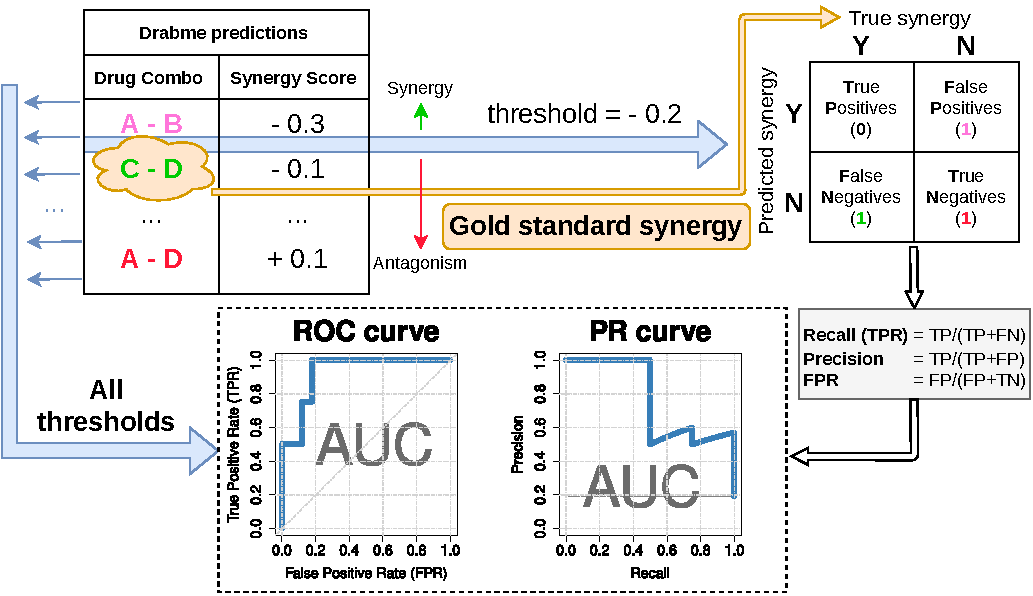
\includegraphics{img/drabme_synergy_roc.pdf}
\caption{\label{fig:fig6}Performance assessment of Drabme's drug synergy predictions. Predicted synergy scores are sorted from synergistic to antagonistic and compared to a gold standard synergy set for several possible thresholds. Each synergy threshold can be used to construct a confusion matrix, from which standard metrics are calculated, such as the number of True Positive (TP) and False Positive (FP) predictions, precision and recall, etc. Visualizing several of these metrics across all thresholds in the Receiver Operating Characteristic (ROC) and Precision Recall (PR) curves, enables the calculation of the Area Under the Curve (AUC), which is a performance score indicating how good the synergy classification method is.}
\end{figure}

While exploring various configuration options for the Gitsbe and Drabme simulations,\footnote{See DrugLogics software documentation \protect\hyperlink{doc-links}{here}} we needed a tool to quickly assess their effect on the pipeline's performance and see which were the most important to tune.
The pipeline's performance here refers to Drabme's output synergy predictions (continuous scores, each one for a different drug combination, ranging from negative and more synergistic values, to positive and more antagonistic values), validated against the computationally derived set of synergistic drug combinations for the AGS cell line (gold standard).
This is a typical binary classification problem, where an imaginary threshold scans the range of Drabme's predicted synergy scores to derive various performance scores.
Specifically, each threshold demarcates the synergistic drug combinations from the antagonistic ones, based on the output prediction scores.
By comparing these assessments with what we consider as the actual truth, i.e.~the gold standard synergy set, a confusion matrix can be constructed and several threshold-specific measures calculated (Figure \ref{fig:fig6}).
By accounting for every such threshold, ranging from a very strict (every prediction is declared as antagonistic) to a very relaxed one (every prediction is declared as synergistic), we can visualize Drabme's classifier performance with the Receiver Operating Characteristic (ROC) {[}\protect\hyperlink{ref-Fawcett2006}{119}{]} and Precision Recall (PR) {[}\protect\hyperlink{ref-Saito2015}{120}{]} curves, which are both well-known diagnostic tools for binary classification problems.
In particular, they allow for a more broad, threshold-agnostic performance measurement, which is the Area Under the Curve (AUC).
An AUC score of 1 is considered as the perfect classification, which in our case would happen if the top most negative synergy scores were exactly the ones corresponding to the drug combinations that represent the gold standard set for the AGS cell line.
The aforementioned diagnostic curves also enable the calculation of ``optimal'' cutpoints, e.g.~thresholds that maximize or minimize certain criteria, an example of the latter being the distance from the point of perfect classification {[}\protect\hyperlink{ref-Perkins2006}{121}{]}.
Based on this theoretical framework, we developed the \texttt{R} shiny app {[}\protect\hyperlink{ref-Chang2021}{122}{]} \texttt{druglogics-roc} to automatically parse Drabme's output files and produce a table {[}\protect\hyperlink{ref-Xie2021}{123}{]} with the confusion matrix values per synergy threshold, along with interactive plots of the ROC (using the \texttt{R} package \texttt{plotly} {[}\protect\hyperlink{ref-Sievert2020}{124}{]}) and PR curves (using the \texttt{R} package \texttt{PRROC} {[}\protect\hyperlink{ref-Grau2015}{125}{]}) and their respective AUC scores.
This app is now part of the DrugLogics software suite,\footnote{See \texttt{druglogics-roc} repository \protect\hyperlink{druglogics-soft-links}{here}} facilitating the visualization of the pipeline's performance.

The Boolean model ensembles produced by Gitsbe were a unique source for further data analyses.
Since such an ensemble contains a large variety of models, all representing the same biological system, we investigated how these models differ in terms of each network node's activity (in the respective attractor) and parameterization.
Moreover, we were interested in how these types of model differences translate to variations in prediction performance, i.e.~make some models predict specific drug combinations as synergistic or not.
By assigning Gitsbe models into different classes based on their individual prediction performance, we could identify nodes that were relatively more active (or inhibited) in the upper tier models compared to the lower tier models of the performance hierarchy.
For example, we verified across many analyses\footnote{See \texttt{gitsbe-model-analysis} repository \protect\hyperlink{misc-links}{here}} that the ERK node of the CASCADE signaling network was particularly overexpressed in the models that predicted most of the gold standard synergies in the AGS cell line from the reference drug combination dataset.
This was an interesting finding, since knowledge gathered from the scientific literature indicates conflicting measurements of ERK activity in AGS cells {[}\protect\hyperlink{ref-Flobak2015}{90}{]} and so our modeling results, upon further analysis, have the potential of providing useful information related to the studied biological system (this particular result is also shown using a different methodology in \textbf{\protect\hyperlink{Paper3}{Paper 3}}).
In addition to the activity-based analyses, we also explored differences with respect to the Boolean model parameterization, i.e.~if higher performance models tend to have specific logical operators (or not) in some equations.
This also motivated us to study how the diversity in particular Boolean rule assignments in the different model classes translates to the respective target nodes' activity (the link between node parameterization and activity was further investigated in \textbf{\protect\hyperlink{Paper5}{Paper 5}}).
To enable all the aforementioned investigations, we began writing functions in several scripts while getting familiar with the world of professional software development in \texttt{R} {[}\protect\hyperlink{ref-Wickham2015}{126}{]}.
In the end, we spent considerable effort to organize all these functions into a single, \emph{clean}, modularized and tested codebase, with the purpose to fill in a niche for data analysis-oriented software that performs auxiliary automated analyses on Boolean model datasets.
The result was the creation of the emba \texttt{R} package and its addition to the DrugLogics software suite (\textbf{\protect\hyperlink{Paper4}{Paper 4}}).

\newpage

\hypertarget{gtrr}{%
\section*{Get the right rules}\label{gtrr}}
\addcontentsline{toc}{section}{Get the right rules}

\indent

In the previous chapter we described in detail all the different requirements that a software needs to satisfy so as to deliver on its promise to \emph{do what it was made to do}.
In other words, it is entirely the software developer's responsibility to make sure that the underlying algorithms are programmed correctly, the model equations and their solutions are correct and that in general, the software works as expected.
In the case of our modeling pipeline, this translates for example to the precise and error-free implementation of the genetic algorithm as well as taking the extra effort to test and ensure that the Boolean models are assigned the desired parameterization and their attractors are correctly calculated.
The aforementioned procedure is semantically synonymous to \emph{verification}: the software works in a manner that directly reflects the underlying theories and modeling assumptions.
This is part of what makes the simulation results trustworthy and actionable, in the sense that they can be used to provide solutions to real-world problems, making the respective models valuable for diverse applications, both in industrial and clinical contexts.

It is a totally different matter if the solutions that the software was made to produce, (e.g.~the simulation results in the case of modeling software), are pragmatic.
What good are models if their outputs do not agree with real observations, no matter how skillfully the developer translated the theoretical ideas in software code?
All models are wrong since they are approximate representations of reality, but they should at least have some use and therefore it is important to be able to pinpoint exactly where this wrongness originates and what it pertains to.
If a biological model for example cannot reproduce basic observations about the phenotype of the system it simulates (via its respective software), then that model is not useful and it probably needs further refinement.
That leads to the question of what makes a model able to better match experimental data and become a more faithful approximation of reality.
In other words, what aspect of the model needs refinement?
The first step towards answering this question is understanding that a model is more than just the code.
A model, as explained in a previous chapter, is a set of mathematical rules applied to a list of biological entities (also referred to as model parameterization).
So, extra care should be given to make sure we have the right equations in our models.
This crucial next step is known as the \emph{validation} of the modeling software and its basic assumption is that more ``right'' equations result in better fit to observations, which lead to better models (their behavior corresponds more accurately to reality) and subsequently, better simulation results (predictions about the studied system).

So for every modeling application and subsequent software, not only do we need to have the rules right (verification), but it is of equal or maybe even more significance to have the right rules (validation) {[}\protect\hyperlink{ref-Roache1997}{127}{]}.
In that aspect, the parameterization of the Boolean models in our software, i.e.~the choice of logical equations that define the regulatory activity of every target in the underlying cancer signaling network, stands as one of the most important parts of the ensuing modeling process.
Since parameterization is so important, how can we find which are the ``right'' rules or similarly, how can we distinguish between those that are right versus those that are not (or are less so), so that we can choose the former for our models?
Practically, the way that researchers in the logical modeling community have dealt with this problem is by establishing standard logical equation forms to represent regulatory interactions upon a signaling target {[}\protect\hyperlink{ref-Mendoza2006}{128}{]}.
Based on such a foundation for the initial construction of the logical rules, the next step is to tweak them properly, by changing logical operators and removing/adding variables (regulators), so that a better match with experimental observations can be achieved.
This process of calibrating the rules to fit the respective data can be either the result of manual curation {[}\protect\hyperlink{ref-Flobak2015}{90},\protect\hyperlink{ref-Faure2009}{129},\protect\hyperlink{ref-Niederdorfer2020}{130}{]}, or the outcome of automated computational search for optimal logical equations {[}\protect\hyperlink{ref-Videla2016}{131},\protect\hyperlink{ref-Gjerga2020}{132}{]} (for similar efforts in this thesis see \textbf{\protect\hyperlink{Paper3}{Paper 3}}).
In addition, several other methods are used to convert various input sources to the appropriate Boolean rules, e.g.~by translating molecular interaction maps directly to Boolean models {[}\protect\hyperlink{ref-Aghamiri2020}{133}{]} or user-provided text to suitable logical equations via web-based tools {[}\protect\hyperlink{ref-Helikar2012}{134}{]}.

\vspace{-6pt}

Be it the modelers or the computers that refine and produce the final Boolean equations in the respective models, we reasoned that a proper framework to characterize the Boolean functions that constitute the rules in these models, is currently missing.
The main idea is that, since the mathematical rules are the heart of modeling and we need to have the right rules (or as best as possible) for validating and further refining our models, a proper toolkit is needed to differentiate and choose between the possible parameterization options.
The plethora of potential equations that can be just ``right'' are a direct consequence of the fact that the number of possible parameterizations increases dramatically with the number of regulators {[}\protect\hyperlink{ref-Cury2019}{135}{]}.
In addition, a large number of Boolean equations may fit equally well the experimental observations or it might even be the case that the data are not enough to uniquely define the model equations {[}\protect\hyperlink{ref-Saez-Rodriguez2009}{136}{]}.
Either way, fitting the model to match the expected outputs is just one side of the validation process.
We need to go deeper than that though if we are to reach our goal of finding biologically reasonable and functionally useful rules for our models.
To establish a practical framework assisting in the choice of a particular logical model parameterization, we need to search for ways to expand our knowledge of the rules and gain insights into these from different perspectives.
Following this logic, there are function properties that Boolean mathematics research has thoroughly studied and which, when brought to the context of modeling, can be beneficial for both modelers and software applications that specify or calibrate the rules of a logical model {[}\protect\hyperlink{ref-Cury2019}{135},\protect\hyperlink{ref-Shmulevich2004}{137},\protect\hyperlink{ref-Gherardi2016}{138}{]}.
For example, such properties could be used to investigate if the equations contradict the structure of the underlying regulatory topology (PKN) or that biologically important regulators manifest in the equations as proportionally influential to the respective Boolean output.
Our efforts constitute a first attempt to compile such a list of Boolean function metrics in a unified framework that could be used to refine the search for the optimal rules to use (\textbf{\protect\hyperlink{Paper5}{Paper 5}}).
The analyses in that paper also show the differences between varying Boolean parameterizations in terms of expected output behavior and how this information, when known \emph{a priori} (based on precise mathematical formalization and subsequent calculation), can assist in the choice of better rules for the considered models.

While establishing a framework to help in the identification of the right rules for a Boolean model, we leveraged the benefits of variation in model parameterization (Figure \ref{fig:fig7}).
Exploring the effects of variation in the values of model parameters, enables the identification of variables which have the largest influence in the behavior of the studied systems and can provide mechanistic insights to explain several phenomena {[}\protect\hyperlink{ref-Aldridge2006}{75}{]}.
For example, in Eduati et al.~(2017) {[}\protect\hyperlink{ref-Eduati2017}{86}{]}, the authors study how logical model parameters are related with cellular sensitivity to anti-cancer drugs.
Simply put, by tweaking a biologically meaningful parameter in their model (the responsiveness of the GSK3 signaling node), you could explain why a drug combination involving a MEK and a GSK3 inhibitor is sensitive in some cancer cell lines and resistant in others.
This computational finding was supported by experimental evidence, thereby providing a proof-of-concept in how the investigation of model parameterization can suggest new mechanisms for the manifestation of particular drug synergies.
On a more theoretical front, in Abou-Jaoudé et al.~(2019) {[}\protect\hyperlink{ref-Abou-Jaoude2019}{139}{]}, the authors formally describe the concept of logical bifurcation diagrams, a framework to assess how changes in the logical parameters result in the change of the dynamics of logical models.
This methodology was used to display the attractors of the simple p53-Mdm2 signaling network as a function of the degradation rate of ubiquitin ligase Mdm2 in the nucleus, allowing for a more concise characterization of its main dynamical properties {[}\protect\hyperlink{ref-Abou-Jaoude2009}{140}{]}.



\begin{figure}
\centering
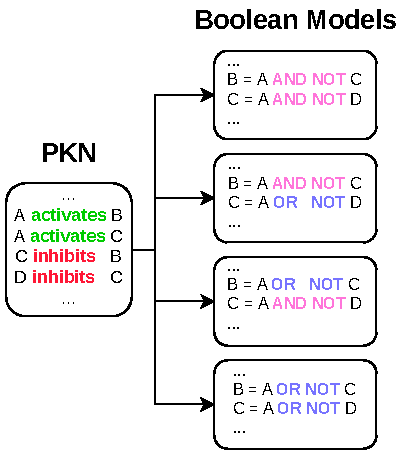
\includegraphics{img/abmlog_simple.pdf}
\caption{\label{fig:fig7}Exploring Boolean model parameterization with the \texttt{abmlog} software. Using as input causal regulatory knowledge, all possible Boolean models that conform to a standardized logical equation form {[}\protect\hyperlink{ref-Mendoza2006}{128}{]} and its most basic variation are produced. Target nodes B and C have two regulators each, and their respective Boolean equations can be formalized in two ways, producing a total of four possible models for further analysis.}
\end{figure}

\newpage

Such approaches inspired us to explore the space of Boolean model parameterization, pertaining to the equations used to construct and mutate the models in the genetic algorithm of Gitsbe (\textbf{\protect\hyperlink{Paper3}{Paper 3}}).
We made a Java software package that can produce either a random sample or all possible Boolean models, based on a standardized equation form {[}\protect\hyperlink{ref-Mendoza2006}{128}{]} and its most basic variation (Figure \ref{fig:fig7}).
The \texttt{abmlog} package is now also part of the DrugLogics software suite and was used in the analyses of \textbf{\protect\hyperlink{Paper5}{Paper 5}} to show how the output behavior of the two alternative parameterization options of the Gitsbe models varies based on the number of regulators in the respective equations and the ratio of positive to negative regulators (as these were defined in the original PKN).
Moreover, a large number of CASCADE-based Boolean models were produced using the \texttt{abmlog} package to explore parameterization variation.
Exploiting the dimension reduction and visualization method UMAP {[}\protect\hyperlink{ref-McInnes2018}{141}{]}, we constructed several Boolean model maps and were able to visualize model differences such as fitness to training data and prediction performance.\footnote{See \texttt{bool-param-maps} repository \protect\hyperlink{misc-links}{here}}
Further analysis identified important nodes which drive the change of dynamics (number of attractors in the CASCADE Boolean models) and whose parameterization could be used to visually separate the UMAP embedded models in distinct clusters.

\newpage

\hypertarget{discussion-future-perspectives}{%
\section*{Discussion \& Future Perspectives}\label{discussion-future-perspectives}}
\addcontentsline{toc}{section}{Discussion \& Future Perspectives}

\indent

In most of the papers included in this thesis there is a separate section discussing potential future tasks, the fulfillment of which will advance the efforts towards achieving the goals of each respective research work.
We also discussed in a previous chapter\footnote{See \protect\hyperlink{psicquic-chapter}{Sharing causal interactions with PSICQUIC}.} additional implementation work that is crucial for establishing a robust infrastructure for the sharing of causal molecular interactions to a wider community of users with PSICQUIC.
Here, we will discuss further implementations and research that needs to be done related to modeling efforts for combating cancer.
First, we will focus on clarifying several aspects in our own computational work and suggest future directions.
Secondly, we will reflect on the more broad problem of understanding cancer and briefly describe the challenges that the computational biology community as a whole needs to overcome to drive future modeling efforts towards enabling more proactive, predictive and personalized Systems Medicine approaches {[}\protect\hyperlink{ref-Hood2011}{84}{]}.

In \textbf{\protect\hyperlink{Paper3}{Paper 3}}, we outline four key prerequisites that a software pipeline designed to construct patient specific logical models should satisfy, in order to facilitate the identification of potential therapeutic solutions for cancer.
These were expressed as (1) assembling a network topology from prior knowledge databases, (2) translating baseline cancer cell line biomarker data into signaling activities, (3) calibrating logical models, created from PKNs, by modifying logical equations to match the observed signaling activities, and (4) predicting phenotypic consequences of combinatorial interventions to the simulated model behavior.
These four generic requirements were embodied in the respective software modules of Figure \ref{fig:fig5}.
Gitsbe and Drabme were our proposed solutions for (3) and (4) and the resulting simulations and analyses was the main scope of \textbf{\protect\hyperlink{Paper3}{Paper 3}}.
Atopo aims to fulfill objective (1) while Aomics is the module that encapsulates the work needed for objective (2).
In the following text, we are going to discuss the reasons why these solutions were not included in \textbf{\protect\hyperlink{Paper3}{Paper 3}} and our future objectives for improvements on the Atopo and Aomics modules.

Starting with the assembly of the PKN, we previously set a list of requirements that such an output network should satisfy to be suitable for our analyses.
These were the inclusion of the drug targets so that they can be perturbed using subsequent pipeline software and the incorporation of major cancer pathways in the PKN.
Atopo is a software module (Figure \ref{fig:fig5}) precisely implemented with these specifications in mind, using SIGNOR's causal molecular interaction data to construct self-contained topologies that include specific signaling entities {[}\protect\hyperlink{ref-Flobak2016}{104}{]}.
The self-contained topology solves a practical issue, since it allows for smaller logical models with fewer fixpoint attractors, increasing computational efficiency.
It is also tightly related to the hypothesis that cancer is a disease system in itself, not dictated by external factors.
Put in other words, whatever makes a cancer cell keep proliferating, comes from within the cell itself.
Moreover, the signaling entities used in Atopo, refer in our case not only to the drug targets, but also to nodes that define the phenotypic output of the computational models later in the pipeline.
In the end, due to the methodology used to prune the network in Atopo and the molecular interaction content included in SIGNOR's database (dated April 2018), the Atopo-generated PKN was hard to make sense of, especially when trying to interpret the simulation results in terms of mechanistic insights.
For example, some analyses using the \texttt{emba} \texttt{R} package from \textbf{\protect\hyperlink{Paper4}{Paper 4}} produced confusing results with regard to the nodes designated as important for the manifestation of particular synergies.\footnote{See \texttt{gitsbe-model-analysis} repository \protect\hyperlink{misc-links}{here}}
Since we had curated the CASCADE family of topologies from literature to incorporate cancer signaling pathways and associated key regulatory targets, it presented itself as a trustable and already refined solution that perfectly fitted our needs.
Our future goal is to combine molecular interaction data from different causal knowledge databases, using software like PSICQUIC {[}\protect\hyperlink{ref-Aranda2011}{61}{]} or OmniPath {[}\protect\hyperlink{ref-Turei2016}{142}{]}, to build larger and more comprehensive PKNs, suitable for our logical modeling applications in the context of cancer signaling.

To derive an accurate activity profile for the signaling entities in CASCADE, we used multiple omics datasets such as copy number alterations (CNA) and expression data (transcriptomics or proteomics) pertaining to each of the cell lines of interest in the reference drug combination dataset chosen for our simulations {[}\protect\hyperlink{ref-Flobak2019}{116}{]}.
These datasets were given as input to appropriate software tools to predict the signaling activity information {[}\protect\hyperlink{ref-Vaske2010}{143}{]}.
Extensive effort was spent in subsequent software, which resulted in the Aomics family of internal tools (Figure \ref{fig:fig5}).
Sadly, we failed to produce reliable signaling activities for the 8 cell lines of the reference drug combination dataset.
For example, model output nodes that are known to be inactivated in cancer cells (e.g.~the family of Caspases), were computed as being active, contradicting basic biological knowledge.
The conversion of various omics datasets to binary signaling information and their efficient integration for modeling purposes is an emerging area of research {[}\protect\hyperlink{ref-Beal2018}{85},\protect\hyperlink{ref-Martignetti2016}{144}--\protect\hyperlink{ref-Dugourd2021}{146}{]}.
We acknowledge the fact that such discretization methodologies might be a bit coarse and ill-suited given the continuous nature of some omics datasets, but they are nonetheless a prerequisite for qualitative modeling methodologies such as ours.
We hope that in the future more standardized methods will be available to handle such datasets and make them better suited for our needs.

Overall, the Aomics endeavor represents a practical example where validation of the various input data sources of a scientific software fails and so, as researchers, we have to use every means available at our disposal to further progress our goals (i.e.~in our case this meant to use a curated PKN and literature-derived signaling observations).
Nonetheless, we can exploit the information presented in such input data sources to further investigate their quality, which can reveal the varying degrees of importance with which such inputs affect the simulation results of the software.
For example, in \textbf{\protect\hyperlink{Paper3}{Paper 3}} we investigated how severely the pipeline's synergy prediction performance was affected by either changes to the input training activity data or the input topology (PKN).
In the end, the results indicated that the topology is far more important, demonstrating the need for high quality prior knowledge and the significance of related curation efforts that translate scientific literature to structured knowledge infrastructures.

\begin{center}\rule{0.5\linewidth}{0.5pt}\end{center}

The work described in this thesis focuses on the qualitative modeling of a single cancer cell, aiming at predicting its phenotypic behavior subject to various drug perturbations.
Our work, along with similar efforts from the Computational Biology community, has only been the first step in the mechanistic modeling of biological systems.
To help scientists better understand cancer cell biology, we need to achieve a better understanding of the processes occurring inside the cell and pave the way for the systematic analysis of cells on a broader scale than what is currently possible.
Up to now, researchers have been constructing, simulating and analyzing models to answer specific questions pertaining to context-specific modeling scenarios.
Such concentrated modeling efforts are usually restrictive, because of their limited scope and the choice of a single mathematical framework to formalize the respective models (e.g.~Boolean mathematics or ODEs).
Thus the resulting biological models are inadequate and can not provide the necessary temporal and spatial resolution of the modeled systems that is required to holistically describe and interpret complex cellular behavior.

There is a gradual shift to replace focused models with larger, multiscale hybrid models.
These types of fine-grained models can incorporate multiple levels of granularity in their associated mathematical representation and simulated molecular scale, and their aim is to provide an accurate description of the cellular phenotype from its respective genotype {[}\protect\hyperlink{ref-Karr2012}{147}{]}.
Such in-silico whole-cell (WC) models are powerful scientific tools that will allow us to identify gaps in our understanding of cell biology and unify our fragmented knowledge of disease development.
Their main advantage is that they can be used to address multiple scientific questions, and conduct complex in-silico experiments that would otherwise be impractical to perform in the laboratory with current technologies.
Such approaches to modeling complex biological systems are foreseen to have a significant impact in a number of applications, both in research and industry (e.g.~biotechnology), serving as a platform to facilitate model-driven discovery {[}\protect\hyperlink{ref-Carrera2015}{148}{]}.
In parallel, research on multicellular modeling aims to improve our understanding of the interactions between the different cells that send and receive signals to communicate and perform tissue- and organism-level functions.
Such models can help us describe in more detail the processes that drive tumor pathogenesis and favor the development and progression of cancer {[}\protect\hyperlink{ref-Senft2017}{149}{]}.
For example, multicellular models could elucidate the mechanisms by which tumor associated macrophages (TAMs) interact with cancer cells in the inflammatory microenvironment of solid tumors {[}\protect\hyperlink{ref-Fukuda2012}{150},\protect\hyperlink{ref-Marku2020}{151}{]}, provide comprehensive explanations of how multicellular cancer resistance manifests {[}\protect\hyperlink{ref-Desoize2000}{152}{]}, and propose novel therapeutic targets that damage the communication of tumor cells with their microenvironment {[}\protect\hyperlink{ref-Komohara2016}{153}{]}.

There exist several challenges in building accurate and comprehensive WC models {[}\protect\hyperlink{ref-whole-cell-doc}{154}{]}.
To fully characterize the function of every gene product and predict the dynamics of all molecular species of a cell over its entire life cycle, WC models need to be able to synthesize information that is subject to different molecular as well as spatiotemporal scales, and perform multi-algorithmic simulations.
Despite the fact that several software tools have been built to enable the construction and simulation of WC models {[}\protect\hyperlink{ref-Tomita1999}{155},\protect\hyperlink{ref-Blinov2017}{156}{]}, a complete integration of all the different algorithmic methodologies representing molecular detail at every possible scale, is currently lacking.
Moreover, a proper theoretical foundation that specifies how the different modeling formalisms can work under a hybrid mathematical framework for WC modeling is also missing {[}\protect\hyperlink{ref-Karr2015}{157}{]}.
On another front, the heterogeneous data needed for the scalable design, construction, calibration, simulation and validation of WC models, are incomplete, imprecise and noisy, calling for the development of new experimental methods and tools to more properly characterize cells at multiple levels of molecular granularity and expression (e.g.~different omics data) {[}\protect\hyperlink{ref-Macklin2020}{158}{]}.
Literature curation tools, used to annotate and extract knowledge from scientific publications, complement the aforementioned efforts by providing a systematic way to assemble the comprehensive prior knowledge that is required for WC modeling.
Therefore, software implementations allowing for new approaches towards the annotation and sharing of causal molecular interactions (as were presented in this thesis), significantly contribute to such efforts.
In addition, we anticipate that the use of machine learning and text mining automated tools are going to be detrimental for future curation efforts, leveraging the vast amounts of biological knowledge for the creation of more accurate WC models.

There are major computational bottlenecks that we need to overcome to enable the comprehensive modeling of complex cells.
Due to the high computational costs required for the calibration and simulation of WC models (e.g.~parameter estimation is particularly resource intensive), high-performance modeling algorithms need to be implemented, along with better parallel processing simulators {[}\protect\hyperlink{ref-Hallock2014}{159}{]}.
Additionally, technological advancements such as cloud and high performance computing (HPC) services {[}\protect\hyperlink{ref-HPC-wiki}{160}{]} will allow us to take advantage of modern computational resources and harness their scalability and processing power, surpassing the limitations of conventional single machines that are unsuitable for such large-scale modeling efforts.
On another front, WC models and their subcomponents (e.g.~signaling pathway models corresponding to distinct cellular processes) need to be interoperable to allow for proper model integration, extension and reuse, as well as enable reproducible simulation results.
During the 2015 WC Modeling Summer School event, efforts directed towards translating a WC model to community formats such as SBML {[}\protect\hyperlink{ref-Keating2020}{161}{]} (for model encoding) and SBGN {[}\protect\hyperlink{ref-Novere2009}{45}{]} (for model visualization), indicated the need for additional standards, databases and software to accelerate WC modeling {[}\protect\hyperlink{ref-Waltemath2016}{162}{]}.

Current approaches to build comprehensive WC models of simple organisms such as the pathogen \emph{Mycoplasma genitalium} {[}\protect\hyperlink{ref-Karr2012}{147},\protect\hyperlink{ref-Burke2020}{163}{]}, and the bacterium \emph{Escherichia Coli} {[}\protect\hyperlink{ref-Carrera2014}{164}{]} constitute significant achievements towards addressing all the aforementioned challenges.
Moreover, they pave the way for the construction of mammalian WC models and eventually whole-organism models {[}\protect\hyperlink{ref-Szigeti2014}{165},\protect\hyperlink{ref-Viceconti2016}{166}{]} (the pinnacle of which should be a complete human model), where the communication and coordination between different WC models (representing different cell types), at different hierarchical levels, is going to be one of the most difficult issues to tackle.
Despite the difficulty inherent in such aspiring projects, many recent research efforts have been focused on studying multicellular systems with potential applications in cancer immunology and therapeutics.
Notably, several tools have been developed using agent-based or similar modeling approaches, providing ways to intuitively represent multicellular biological systems {[}\protect\hyperlink{ref-Ghaffarizadeh2018}{167}--\protect\hyperlink{ref-Stoll2020}{171}{]}.
Such methodologies facilitate the integration of multiple scales for the study of cell population dynamics, and some also incorporate various spatial aspects of the modeled systems.
The respective software simulators make use of coarse-grained characterizations of the interacting cells (i.e.~the agents), significantly reducing the computational simulation costs.
Even though current multicellular models do not encapsulate a realistic picture of the intracellular signaling (since it is impractical to incorporate full WC models) nor of the cell communication mechanics, they have been successfully used to validate several experimental findings and study interacting cells in dynamic tissue microenvironments such as heterogeneous cell tumors.
Moreover, multicellular models have the potential to assist in the exploration of the effects that the genetic alteration of individual cells has to the population level (e.g.~how knocking out genes in specific cells can limit tumor growth), the investigation of response to various anti-cancer treatments, as well as the study of the cellular mechanisms and dynamics of carcinogenesis.
We can only expect that in the future, biological and medical applications will push the boundaries of what is achievable by such software modeling solutions and that multicellular and WC models will drive progress in the cancer-related research areas and beyond.

Lastly, we stress the necessity of interdisciplinarity and collaboration across the research and industrial spectrum, to solve all the grand challenges involved in the modeling of complex biological systems and the efforts to combat diseases such as cancer.
Building a cohesive Computational Biology community also plays an important role, as it promotes a \emph{common vision} and a collaborative spirit amongst the members of the community.
The success story of the COMBINE initiative's standardization efforts in computational biological modeling, has been empowered by the promotion of its standards via tutorials, workshops and dedicated sessions at international conferences {[}\protect\hyperlink{ref-Hucka2015}{172}{]}.
As scientists, we are called to take risks, not only to explore the unknown and yet uncharted territory of our world but also to face the social and communication challenges between ourselves.
Only together, as one community, can we set the world in order, tackle the problems of today, and make a better tomorrow for all humankind.

\hypertarget{appendix-appendix}{%
\appendix}


\hypertarget{links-to-software-documentation-and-data-analyses}{%
\chapter*{Links to software, documentation and data analyses}\label{links-to-software-documentation-and-data-analyses}}
\addcontentsline{toc}{chapter}{Links to software, documentation and data analyses}

\vspace{-10pt}

\hypertarget{github-org-links}{%
\section*{GitHub organizations}\label{github-org-links}}
\addcontentsline{toc}{section}{GitHub organizations}

\begin{itemize}
\tightlist
\item
  UniBioDicts: \url{https://github.com/UniBioDicts/}
\item
  VSM: \url{https://github.com/vsm}
\item
  DrugLogics: \url{https://github.com/druglogics}
\item
  PSICQUIC: \url{https://github.com/PSICQUIC}
\end{itemize}

\hypertarget{doc-links}{%
\section*{Documentation}\label{doc-links}}
\addcontentsline{toc}{section}{Documentation}

\begin{itemize}
\tightlist
\item
  DrugLogics software: \url{https://druglogics.github.io/druglogics-doc/}
\item
  VSM technology and related projects: \url{https://vsm.github.io/}
\item
  PSICQUIC: \url{https://psicquic.github.io/}
\end{itemize}

\hypertarget{druglogics-soft-links}{%
\section*{DrugLogics software modules}\label{druglogics-soft-links}}
\addcontentsline{toc}{section}{DrugLogics software modules}

\begin{itemize}
\tightlist
\item
  \href{https://github.com/druglogics/gitsbe}{\texttt{gitsbe}}: A Java module that defines Boolean models compliant with observed behavior (e.g.~steady state or perturbation data) using an automated, model parameterization genetic algorithm
\item
  \href{https://github.com/druglogics/drabme}{\texttt{drabme}}: A Java module that performs a drug perturbation response analysis to the Boolean model ensembles generated by Gitsbe
\item
  \href{https://github.com/druglogics/druglogics-synergy}{\texttt{druglogics-synergy}}: A Java module to execute serially Gitsbe and then Drabme
\item
  \href{https://github.com/druglogics/abmlog}{\texttt{abmlog}}: A Java-based generator of all possible logical models with AND/OR-NOT link operators in their respective Boolean equations (Figure \ref{fig:fig7})
\item
  \href{https://github.com/druglogics/druglogics-roc}{\texttt{druglogics-roc}}: \texttt{R} Shiny web app to visualize the ROC and PR prediction performance of Drabme's ensemble-wise predictions (Figure \ref{fig:fig6})
\item
  \href{https://github.com/bblodfon/emba/}{\texttt{emba}}: \texttt{R} package for analysis and visualization of biomarkers in Boolean model ensembles {[}\protect\hyperlink{ref-Zobolas2020}{3}{]}
\end{itemize}

\hypertarget{r-community-packages}{%
\section*{R community packages}\label{r-community-packages}}
\addcontentsline{toc}{section}{R community packages}

\begin{itemize}
\tightlist
\item
  \href{https://github.com/bblodfon/usefun}{\texttt{usefun}}: various useful \texttt{R} functions
\item
  \href{https://github.com/bblodfon/rtemps}{\texttt{rtemps}}: templates for reproducible data analyses with \texttt{R} {[}\protect\hyperlink{ref-rtemps}{173}{]}
\end{itemize}

\hypertarget{misc-links}{%
\section*{Miscellaneous data analyses and repositories}\label{misc-links}}
\addcontentsline{toc}{section}{Miscellaneous data analyses and repositories}

All the following repositories have been authored exclusively by myself.
Each repository has a \texttt{README.md} file with a brief description of the analysis and a link to online documentation and results (in the form of \texttt{R} Markdown documents or \texttt{R} GitBooks).

\begin{itemize}
\tightlist
\item
  \href{https://github.com/druglogics/cascade}{\texttt{cascade}}: repository of the different versions of the CAncer Signaling CAusality DatabasE developed by the DrugLogics group
\item
  \href{https://github.com/druglogics/ags-paper}{\texttt{ags-paper}}: simulation results and data analyses related to \textbf{\protect\hyperlink{Paper3}{Paper 3}}
\item
  \href{https://github.com/druglogics/sintef-obs-synergies}{\texttt{sintef-obs-synergies}}: synergy assessment of the Flobak et al.~(2019) {[}\protect\hyperlink{ref-Flobak2019}{116}{]} drug combination dataset using rbbt {[}\protect\hyperlink{ref-Vazquez2010}{174}{]} and the CImbinator tool {[}\protect\hyperlink{ref-Flobak2017}{117}{]}
\item
  \href{https://github.com/druglogics/brf-bias}{\texttt{brf-bias}}: data analyses related to the study of truth density bias in standardized Boolean regulatory functions for \textbf{\protect\hyperlink{Paper5}{Paper 5}}
\item
  \href{https://github.com/druglogics/gitsbe-model-analysis}{\texttt{gitsbe-model-analysis}}: several analyses using Boolean model ensemble datasets generated via Gitsbe and the emba \texttt{R} package to analyze them
\item
  \href{https://github.com/druglogics/bool-param-maps}{\texttt{bool-param-maps}}: visualization of model parameterization and node importance using UMAP and random forests on the CASCADE 1.0 Boolean model dataset generated by \texttt{abmlog}
\end{itemize}

\hypertarget{references}{%
\chapter*{References}\label{references}}
\addcontentsline{toc}{chapter}{References}

\hypertarget{refs}{}
\begin{CSLReferences}{1}{0}
\leavevmode\hypertarget{ref-UBDs}{}%
1. Zobolas, J., Touré, V., Kuiper, M., \& Vercruysse, S. (2020). {UniBioDicts: Unified access to Biological Dictionaries}. \emph{Bioinformatics}, \emph{37}(1), 143--144. \url{https://doi.org/10.1093/bioinformatics/btaa1065}

\leavevmode\hypertarget{ref-Zobolas2020-pubdict}{}%
2. Zobolas, J., Kim, J.-D., Kuiper, M., \& Vercruysse, S. (2020). \emph{{Linking PubDictionaries with UniBioDicts to support Community Curation}}. BioHackrXiv. \url{https://doi.org/10.37044/osf.io/gzfa8}

\leavevmode\hypertarget{ref-Zobolas2020}{}%
3. Zobolas, J., Kuiper, M., \& Flobak, Å. (2020). {emba: R package for analysis and visualization of biomarkers in boolean model ensembles}. \emph{Journal of Open Source Software}, \emph{5}(53), 2583. \url{https://doi.org/10.21105/joss.02583}

\leavevmode\hypertarget{ref-Zobolas2021-bias}{}%
4. Zobolas, J., Monteiro, P. T., Kuiper, M., \& Flobak, Å. (2021). \emph{{Boolean function metrics can assist modelers to check and choose logical rules}}. \url{http://arxiv.org/abs/2104.01279}

\leavevmode\hypertarget{ref-vsm-box}{}%
5. Vercruysse, S., Zobolas, J., Touré, V., Andersen, M. K., \& Kuiper, M. (2020). {VSM-box: general-purpose interface for biocuration and knowledge representation}. \emph{Preprints}. \url{https://doi.org/10.20944/preprints202007.0557.v1}

\leavevmode\hypertarget{ref-Toure2021}{}%
6. Touré, V., Zobolas, J., Kuiper, M., \& Vercruysse, S. (2021). {CausalBuilder: bringing the MI2CAST causal interaction annotation standard to the curator}. \emph{Database}. \url{https://doi.org/10.1093/database/baaa107}

\leavevmode\hypertarget{ref-Perfetto2019}{}%
7. Perfetto, L., Acencio, M. L., Bradley, G., Cesareni, G., Del Toro, N., Fazekas, D., Hermjakob, H., Korcsmaros, T., Kuiper, M., Lægreid, A., Lo Surdo, P., Lovering, R. C., Orchard, S., Porras, P., Thomas, P. D., Touré, V., Zobolas, J., \& Licata, L. (2019). {CausalTAB: the PSI-MITAB 2.8 updated format for signalling data representation and dissemination}. \emph{Bioinformatics}. \url{https://doi.org/10.1093/bioinformatics/btz132}

\leavevmode\hypertarget{ref-Abbate2000}{}%
8. Abbate, J. (2000). \emph{{Inventing the internet}}. MIT press.

\leavevmode\hypertarget{ref-Naughton2016}{}%
9. Naughton, J. (2016). {The evolution of the Internet: from military experiment to General Purpose Technology}. \emph{Journal of Cyber Policy}, \emph{1}(1), 5--28. \url{https://doi.org/10.1080/23738871.2016.1157619}

\leavevmode\hypertarget{ref-Polasky2019}{}%
10. Polasky, S., Kling, C. L., Levin, S. A., Carpenter, S. R., Daily, G. C., Ehrlich, P. R., Heal, G. M., \& Lubchenco, J. (2019). {Role of economics in analyzing the environment and sustainable development}. \emph{Proceedings of the National Academy of Sciences of the United States of America}, \emph{116}(12), 5233--5238. \url{https://doi.org/10.1073/pnas.1901616116}

\leavevmode\hypertarget{ref-Roser2013}{}%
11. Roser, M., Ortiz-Ospina, E., \& Ritchie, H. (2013). \emph{{Life Expectancy}}. \url{https://ourworldindata.org/life-expectancy} (15 May 2021, date last accessed).

\leavevmode\hypertarget{ref-Jinek2012}{}%
12. Jinek, M., Chylinski, K., Fonfara, I., Hauer, M., Doudna, J. A., \& Charpentier, E. (2012). {A programmable dual-RNA--guided DNA endonuclease in adaptive bacterial immunity}. \emph{Science}, \emph{337}(6096), 816--821.

\leavevmode\hypertarget{ref-Zhu2020}{}%
13. Zhu, H., Li, C., \& Gao, C. (2020). {Applications of CRISPR--Cas in agriculture and plant biotechnology}. \emph{Nature Reviews Molecular Cell Biology}, \emph{21}(11), 661--677. \url{https://doi.org/10.1038/s41580-020-00288-9}

\leavevmode\hypertarget{ref-Bailey2020}{}%
14. Bailey, R., \& Tupy, M. L. (2020). \emph{{Ten Global Trends Every Smart Person Should Know: And Many Others You Will Find Interesting}}. Cato Institute.

\leavevmode\hypertarget{ref-Gibbons1999}{}%
15. Gibbons, M. (1999). {Science's new social contract with society}. \emph{Nature}, \emph{402}, C81--C84. \url{https://doi.org/10.1038/35011576}

\leavevmode\hypertarget{ref-HAQ2015}{}%
16. \emph{{Healthcare Access and Quality Index}}. (2015). \url{https://ourworldindata.org/grapher/healthcare-access-and-quality-index} (15 May 2021, date last accessed).

\leavevmode\hypertarget{ref-Apweiler2018}{}%
17. Apweiler, R., Beissbarth, T., Berthold, M. R., Blüthgen, N., Burmeister, Y., Dammann, O., Deutsch, A., Feuerhake, F., Franke, A., Hasenauer, J., Hoffmann, S., Höfer, T., Jansen, P. L., Kaderali, L., Klingmüller, U., Koch, I., Kohlbacher, O., Kuepfer, L., Lammert, F., \ldots{} Wolkenhauer, O. (2018). {Whither systems medicine?} \emph{Experimental {\&} Molecular Medicine}, \emph{50}(3), e453. \url{https://doi.org/10.1038/emm.2017.290}

\leavevmode\hypertarget{ref-Trudeau1976}{}%
18. Trudeau, R. J. (1976). \emph{{Dots and lines}}. Kent State University Press.

\leavevmode\hypertarget{ref-Erdos1960}{}%
19. Erdos, P., \& Rényi, A. (1960). {On the evolution of random graphs}. \emph{Publ. Math. Inst. Hung. Acad. Sci}, \emph{5}(1), 17--60.

\leavevmode\hypertarget{ref-Barabasi1999}{}%
20. Barabási, A. L., \& Albert, R. (1999). {Emergence of scaling in random networks}. \emph{Science}, \emph{286}(5439), 509--512. \url{https://doi.org/10.1126/science.286.5439.509}

\leavevmode\hypertarget{ref-Barabasi2013}{}%
21. Barabási, A. L. (2013). {Network science}. \emph{Philosophical Transactions of the Royal Society A: Mathematical, Physical and Engineering Sciences}, \emph{371}(1987). \url{https://doi.org/10.1098/rsta.2012.0375}

\leavevmode\hypertarget{ref-Csardi2006}{}%
22. Csardi, G., \& Nepusz, T. (2006). {The igraph software package for complex network research}. \emph{InterJournal, Complex Systems}, \emph{1695}(5), 1--9. \url{http://igraph.org}

\leavevmode\hypertarget{ref-Bastian2009}{}%
23. Bastian, M., Heymann, S., \& Jacomy, M. (2009). {Gephi: an open source software for exploring and manipulating networks}. \emph{Proceedings of the International AAAI Conference on Web and Social Media}.

\leavevmode\hypertarget{ref-Mrvar2016}{}%
24. Mrvar, A., \& Batagelj, V. (2016). {Analysis and visualization of large networks with program package Pajek}. \emph{Complex Adaptive Systems Modeling}, \emph{4}(1), 1--8. \url{https://doi.org/10.1186/s40294-016-0017-8}

\leavevmode\hypertarget{ref-Shannon2003}{}%
25. Shannon, P., Markiel, A., Ozier, O., Baliga, N. S., Wang, J. T., Ramage, D., Amin, N., Schwikowski, B., \& Ideker, T. (2003). {Cytoscape: a software environment for integrated models of biomolecular interaction networks}. \emph{Genome Research}, \emph{13}(11), 2498--2504.

\leavevmode\hypertarget{ref-Dahlquist2002}{}%
26. Dahlquist, K. D., Salomonis, N., Vranizan, K., Lawlor, S. C., \& Conklin, B. R. (2002). {GenMAPP, a new tool for viewing and analyzing microarray data on biological pathways}. \emph{Nature Genetics}, \emph{31}(1), 19--20. \url{https://doi.org/10.1038/ng0502-19}

\leavevmode\hypertarget{ref-Breitkreutz2003}{}%
27. Breitkreutz, B.-J., Stark, C., \& Tyers, M. (2003). {Osprey: a network visualization system}. \emph{Genome Biology}, \emph{4}(3), R22. \url{https://doi.org/10.1186/gb-2003-4-3-r22}

\leavevmode\hypertarget{ref-Funahashi2003}{}%
28. Funahashi, A., Morohashi, M., Kitano, H., \& Tanimura, N. (2003). {CellDesigner: a process diagram editor for gene-regulatory and biochemical networks}. \emph{BIOSILICO}, \emph{1}(5), 159--162. \url{https://doi.org/10.1016/s1478-5382(03)02370-9}

\leavevmode\hypertarget{ref-Sidiropoulos2017}{}%
29. Sidiropoulos, K., Viteri, G., Sevilla, C., Jupe, S., Webber, M., Orlic-Milacic, M., Jassal, B., May, B., Shamovsky, V., Duenas, C., Rothfels, K., Matthews, L., Song, H., Stein, L., Haw, R., D'Eustachio, P., Ping, P., Hermjakob, H., \& Fabregat, A. (2017). {Reactome enhanced pathway visualization}. \emph{Bioinformatics}, \emph{33}(21), 3461--3467. \url{https://doi.org/10.1093/bioinformatics/btx441}

\leavevmode\hypertarget{ref-Smith2009}{}%
30. Smith, M. A., Shneiderman, B., Milic-Frayling, N., Mendes Rodrigues, E., Barash, V., Dunne, C., Capone, T., Perer, A., \& Gleave, E. (2009). {Analyzing (social media) networks with NodeXL}. \emph{Proceedings of the Fourth International Conference on Communities and Technologies - c{\&}t '09}, 255. \url{https://doi.org/10.1145/1556460.1556497}

\leavevmode\hypertarget{ref-Kalamaras2014}{}%
31. Kalamaras, D. (2014). \emph{{Social Networks Visualizer (SocNetV): Social network analysis and visualization software}}. \url{http://socnetv.org}

\leavevmode\hypertarget{ref-Chatterjee2021}{}%
32. Chatterjee, T., Albert, R., Thapliyal, S., Azarhooshang, N., \& DasGupta, B. (2021). {Detecting network anomalies using Forman--Ricci curvature and a case study for human brain networks}. \emph{Scientific Reports}, \emph{11}(1), 8121. \url{https://doi.org/10.1038/s41598-021-87587-z}

\leavevmode\hypertarget{ref-Mislove2007}{}%
33. Mislove, A., Marcon, M., Gummadi, K. P., Druschel, P., \& Bhattacharjee, B. (2007). {Measurement and analysis of online social networks}. \emph{Proceedings of the ACM SIGCOMM Internet Measurement Conference, IMC}, 29--42. \url{https://doi.org/10.1145/1298306.1298311}

\leavevmode\hypertarget{ref-Maheshwari2020}{}%
34. Maheshwari, P., \& Albert, R. (2020). {Network model and analysis of the spread of Covid-19 with social distancing}. \emph{Applied Network Science}, \emph{5}(1), 1--13. \url{https://doi.org/10.1007/s41109-020-00344-5}

\leavevmode\hypertarget{ref-Barabasi2011}{}%
35. Barabási, A.-L., Gulbahce, N., \& Loscalzo, J. (2011). {Network medicine: a network-based approach to human disease.} \emph{Nature Reviews. Genetics}, \emph{12}(1), 56--68. \url{https://doi.org/10.1038/nrg2918}

\leavevmode\hypertarget{ref-Vercruysse2019a}{}%
36. Vercruysse, S. (2019). \emph{{VSM Pages}}. \url{https://vsm.github.io/vsm-pages/intro} (15 May 2021, date last accessed).

\leavevmode\hypertarget{ref-Howe2008}{}%
37. Howe, D., Costanzo, M., Fey, P., Gojobori, T., Hannick, L., Hide, W., Hill, D. P., Kania, R., Schaeffer, M., St Pierre, S., Twigger, S., White, O., \& Yon Rhee, S. (2008). {Big data: The future of biocuration}. \emph{Nature}, \emph{455}(7209), 47--50. \url{https://doi.org/10.1038/455047a}

\leavevmode\hypertarget{ref-Ammari2018}{}%
38. Ammari, M., Chatr Aryamontri, A., Attrill, H., Bairoch, A., Berardini, T., Blake, J., Chen, Q., Collado, J., Dauga, D., Dudley, J. T., Engel, S., Erill, I., Fey, P., Gibson, R., Hermjakob, H., Holliday, G., Howe, D., Hunter, C., Landsman, D., \ldots{} Zhang, Z. (2018). {Biocuration: Distilling data into knowledge}. \emph{PLOS Biology}, \emph{16}(4), e2002846. \url{https://doi.org/10.1371/journal.pbio.2002846}

\leavevmode\hypertarget{ref-Jenssen2001}{}%
39. Jenssen, T.-K., Lægreid, A., Komorowski, J., \& Hovig, E. (2001). {A literature network of human genes for high-throughput analysis of gene expression}. \emph{Nature Genetics}, \emph{28}(1), 21--28. \url{https://doi.org/10.1038/ng0501-21}

\leavevmode\hypertarget{ref-intact-editor}{}%
40. \emph{{IntAct editor}}. (2007). \url{https://github.com/EBI-IntAct/intact-editor} (15 May 2021, date last accessed).

\leavevmode\hypertarget{ref-Rutherford2014}{}%
41. Rutherford, K. M., Harris, M. A., Lock, A., Oliver, S. G., \& Wood, V. (2014). {Canto: an online tool for community literature curation}. \emph{Bioinformatics}, \emph{30}(12), 1791--1792. \url{https://doi.org/10.1093/bioinformatics/btu103}

\leavevmode\hypertarget{ref-canto-doc}{}%
42. \emph{{Canto Documentation}}. (2014). \url{https://curation.pombase.org/pombe/docs/index/}, (15 May 2021, date last accessed).

\leavevmode\hypertarget{ref-Kuperstein2013}{}%
43. Kuperstein, I., Cohen, D. P. A., Pook, S., Viara, E., Calzone, L., Barillot, E., \& Zinovyev, A. (2013). {NaviCell: A web-based environment for navigation, curation and maintenance of large molecular interaction maps}. \emph{BMC Systems Biology}, \emph{7}(1), 100. \url{https://doi.org/10.1186/1752-0509-7-100}

\leavevmode\hypertarget{ref-Gawron2016}{}%
44. Gawron, P., Ostaszewski, M., Satagopam, V., Gebel, S., Mazein, A., Kuzma, M., Zorzan, S., McGee, F., Otjacques, B., Balling, R., \& Schneider, R. (2016). {MINERVA---A platform for visualization and curation of molecular interaction networks}. \emph{Npj Systems Biology and Applications}, \emph{2}(1), 1--6. \url{https://doi.org/10.1038/npjsba.2016.20}

\leavevmode\hypertarget{ref-Novere2009}{}%
45. Novère, N. L., Hucka, M., Mi, H., Moodie, S., Schreiber, F., Sorokin, A., Demir, E., Wegner, K., Aladjem, M. I., Wimalaratne, S. M., Bergman, F. T., Gauges, R., Ghazal, P., Kawaji, H., Li, L., Matsuoka, Y., Villéger, A., Boyd, S. E., Calzone, L., \ldots{} Kitano, H. (2009). {The Systems Biology Graphical Notation}. \emph{Nature Biotechnology}, \emph{27}(8), 735--741. \url{https://doi.org/10.1038/nbt.1558}

\leavevmode\hypertarget{ref-vsm-paper}{}%
46. Vercruysse, S., \& Kuiper, M. (2020). {Intuitive representation of computable knowledge}. \emph{Preprints}. \url{https://doi.org/10.20944/preprints202007.0486.v2}

\leavevmode\hypertarget{ref-Toure2020}{}%
47. Touré, V., Vercruysse, S., Acencio, M. L., Lovering, R., Orchard, S., Bradley, G., Casals-Casas, C., Chaouiya, C., Del-Toro, N., Flobak, Å., Gaudet, P., Hermjakob, H., Licata, L., Lægreid, A., Mungall, C., Niknejad, A., Panni, S., Perfetto, L., Porras, P., \ldots{} Kuiper, M. (2020). {The Minimum Information about a Molecular Interaction Causal Statement (MI2CAST)}. \emph{Bioinformatics}. \url{https://doi.org/10.1093/bioinformatics/btaa622}

\leavevmode\hypertarget{ref-mi2cast-doc}{}%
48. Vasundra, T. (2020). \emph{{MI2CAST Documentation}}. \url{https://github.com/MI2CAST/MI2CAST/blob/master/docs/MI2CAST_guideline.md} (15 May 2021, date last accessed).

\leavevmode\hypertarget{ref-TheUniProtConsortium2019}{}%
49. The UniProt Consortium. (2019). {UniProt: a worldwide hub of protein knowledge}. \emph{Nucleic Acids Research}, \emph{47}(D1), D506--D515. \url{https://doi.org/10.1093/nar/gky1049}

\leavevmode\hypertarget{ref-Meldal2019}{}%
50. Meldal, B. H. M., Bye-A-Jee, H., Gajdoš, L., Hammerová, Z., Horáčková, A., Melicher, F., Perfetto, L., Pokorný, D., Lopez, M. R., Türková, A., Wong, E. D., Xie, Z., Casanova, E. B., Del-Toro, N., Koch, M., Porras, P., Hermjakob, H., \& Orchard, S. (2019). {Complex Portal 2018: extended content and enhanced visualization tools for macromolecular complexes}. \emph{Nucleic Acids Research}, \emph{47}(D1), D550--D558. \url{https://doi.org/10.1093/nar/gky1001}

\leavevmode\hypertarget{ref-RNACentral2018}{}%
51. The RNAcentral Consortium. (2018). {RNAcentral: a hub of information for non-coding RNA sequences}. \emph{Nucleic Acids Research}, \emph{47}(D1), D1250--D1251. \url{https://doi.org/10.1093/nar/gky1206}

\leavevmode\hypertarget{ref-Whetzel2011}{}%
52. Whetzel, P. L., Noy, N. F., Shah, N. H., Alexander, P. R., Nyulas, C., Tudorache, T., \& Musen, M. A. (2011). {BioPortal: enhanced functionality via new Web services from the National Center for Biomedical Ontology to access and use ontologies in software applications.} \emph{Nucleic Acids Research}, \emph{39}(Web Server issue), W541--5. \url{https://doi.org/10.1093/nar/gkr469}

\leavevmode\hypertarget{ref-Madeira2019}{}%
53. Madeira, F., Park, Y. mi, Lee, J., Buso, N., Gur, T., Madhusoodanan, N., Basutkar, P., Tivey, A. R. N., Potter, S. C., Finn, R. D., \& Lopez, R. (2019). {The EMBL-EBI search and sequence analysis tools APIs in 2019}. \emph{Nucleic Acids Research}, \emph{47}(W1), W636--W641. \url{https://doi.org/10.1093/nar/gkz268}

\leavevmode\hypertarget{ref-Wilkinson2016}{}%
54. Wilkinson, M. D., Dumontier, M., Aalbersberg, Ij. J., Appleton, G., Axton, M., Baak, A., Blomberg, N., Boiten, J. W., da Silva Santos, L. B., Bourne, P. E., Bouwman, J., Brookes, A. J., Clark, T., Crosas, M., Dillo, I., Dumon, O., Edmunds, S., Evelo, C. T., Finkers, R., \ldots{} Mons, B. (2016). {The FAIR Guiding Principles for scientific data management and stewardship}. \emph{Scientific Data}, \emph{3}(1), 1--9. \url{https://doi.org/10.1038/sdata.2016.18}

\leavevmode\hypertarget{ref-Hartmann2019}{}%
55. Hartmann, N. B., Hüffer, T., Thompson, R. C., Hassellöv, M., Verschoor, A., Daugaard, A. E., Rist, S., Karlsson, T., Brennholt, N., Cole, M., Herrling, M. P., Hess, M. C., Ivleva, N. P., Lusher, A. L., \& Wagner, M. (2019). {Are We Speaking the Same Language? Recommendations for a Definition and Categorization Framework for Plastic Debris}. \emph{Environmental Science and Technology}, \emph{53}(3), 1039--1047. \url{https://doi.org/10.1021/acs.est.8b05297}

\leavevmode\hypertarget{ref-Kim2019}{}%
56. Kim, J.-D., Wang, Y., Fujiwara, T., Okuda, S., Callahan, T. J., \& Cohen, K. B. (2019). {Open Agile text mining for bioinformatics: the PubAnnotation ecosystem}. \emph{Bioinformatics}, \emph{35}(21), 4372--4380. \url{https://doi.org/10.1093/bioinformatics/btz227}

\leavevmode\hypertarget{ref-Hermjakob2004}{}%
57. Hermjakob, H., Montecchi-Palazzi, L., Bader, G., Wojcik, J., Salwinski, L., Ceol, A., Moore, S., Orchard, S., Sarkans, U., Mering, C. von, Roechert, B., Poux, S., Jung, E., Mersch, H., Kersey, P., Lappe, M., Li, Y., Zeng, R., Rana, D., \ldots{} Apweiler, R. (2004). {The HUPO PSI's Molecular Interaction format---a community standard for the representation of protein interaction data}. \emph{Nature Biotechnology}, \emph{22}(2), 177--183. \url{https://doi.org/10.1038/nbt926}

\leavevmode\hypertarget{ref-Sivade2018}{}%
58. Sivade, M., Alonso-López, D., Ammari, M., Bradley, G., Campbell, N. H., Ceol, A., Cesareni, G., Combe, C., De Las Rivas, J., Del-Toro, N., Heimbach, J., Hermjakob, H., Jurisica, I., Koch, M., Licata, L., Lovering, R. C., Lynn, D. J., Meldal, B. H. M., Micklem, G., \ldots{} Orchard, S. (2018). {Encompassing new use cases - level 3.0 of the HUPO-PSI format for molecular interactions}. \emph{BMC Bioinformatics}, \emph{19}(1), 134. \url{https://doi.org/10.1186/s12859-018-2118-1}

\leavevmode\hypertarget{ref-Kerrien2007}{}%
59. Kerrien, S., Orchard, S., Montecchi-Palazzi, L., Aranda, B., Quinn, A. F., Vinod, N., Bader, G. D., Xenarios, I., Wojcik, J., Sherman, D., Tyers, M., Salama, J. J., Moore, S., Ceol, A., Chatr-aryamontri, A., Oesterheld, M., Stümpflen, V., Salwinski, L., Nerothin, J., \ldots{} Hermjakob, H. (2007). {Broadening the horizon -- level 2.5 of the HUPO-PSI format for molecular interactions}. \emph{BMC Biology}, \emph{5}(1), 44. \url{https://doi.org/10.1186/1741-7007-5-44}

\leavevmode\hypertarget{ref-Licata2019}{}%
60. Licata, L., Lo Surdo, P., Iannuccelli, M., Palma, A., Micarelli, E., Perfetto, L., Peluso, D., Calderone, A., Castagnoli, L., \& Cesareni, G. (2019). {SIGNOR 2.0, the SIGnaling Network Open Resource 2.0: 2019 update}. \emph{Nucleic Acids Research}. \url{https://doi.org/10.1093/nar/gkz949}

\leavevmode\hypertarget{ref-Aranda2011}{}%
61. Aranda, B., Blankenburg, H., Kerrien, S., Brinkman, F. S. L., Ceol, A., Chautard, E., Dana, J. M., De Las Rivas, J., Dumousseau, M., Galeota, E., Gaulton, A., Goll, J., Hancock, R. E. W., Isserlin, R., Jimenez, R. C., Kerssemakers, J., Khadake, J., Lynn, D. J., Michaut, M., \ldots{} Hermjakob, H. (2011). {PSICQUIC and PSISCORE: accessing and scoring molecular interactions}. \emph{Nature Methods}, \emph{8}(7), 528--529. \url{https://doi.org/10.1038/nmeth.1637}

\leavevmode\hypertarget{ref-mitab28-doc}{}%
62. \emph{{MITAB 2.8 Documentation}}. (2018). \url{http://psicquic.github.io/MITAB28Format.html}, (15 May 2021, date last accessed).

\leavevmode\hypertarget{ref-mi-github}{}%
63. \emph{{Molecular Interactions Community}}. (2015). \url{https://github.com/MICommunity}, (15 May 2021, date last accessed).

\leavevmode\hypertarget{ref-soft-rot-wiki}{}%
64. \emph{{Software rot (Wikipedia entry)}}. (2014). \url{https://en.wikipedia.org/wiki/Software_rot}, (15 May 2021, date last accessed).

\leavevmode\hypertarget{ref-Sivade2018a}{}%
65. Sivade, M., Koch, M., Shrivastava, A., Alonso-López, D., De Las Rivas, J., Del-Toro, N., Combe, C. W., Meldal, B. H. M., Heimbach, J., Rappsilber, J., Sullivan, J., Yehudi, Y., \& Orchard, S. (2018). {JAMI: a Java library for molecular interactions and data interoperability}. \emph{BMC Bioinformatics}, \emph{19}(1), 133. \url{https://doi.org/10.1186/s12859-018-2119-0}

\leavevmode\hypertarget{ref-Hinxton2018}{}%
66. \emph{{GREEKC Hinxton Workshop}}. (2018). \url{https://www.greekc.org/activity/hinxton-workshop/}, (15 May 2021, date last accessed).

\leavevmode\hypertarget{ref-biohack2018}{}%
67. \emph{{ELIXIR BioHackathon Paris}}. (2018). \url{https://2018.biohackathon-europe.org/}, (15 May 2021, date last accessed).

\leavevmode\hypertarget{ref-psicquic-causalTAB-dataset}{}%
68. Del-Toro, N., Zobolas, J., \& Touré, V. (2019). \emph{{Signor Dataset in CausalTAB (PSICQUIC Dev Server)}}. \url{http://wwwdev.ebi.ac.uk/Tools/webservices/psicquic/causality/webservices/current/search/query/*?firstResult=0\&maxResults=10\&format=tab28}, (15 May 2021, date last accessed).

\leavevmode\hypertarget{ref-psicquic-view}{}%
69. \emph{{PSICQUIC View}}. (2011). \url{http://www.ebi.ac.uk/Tools/webservices/psicquic/view/main.xhtml}, (15 May 2021, date last accessed).

\leavevmode\hypertarget{ref-PSICQUICUniversalClient}{}%
70. \emph{{PSICQUIC Universal Client (Cytoscape app)}}. (2012). \url{https://apps.cytoscape.org/apps/psicquicuniversalclient}, (15 May 2021, date last accessed).

\leavevmode\hypertarget{ref-Millan2013}{}%
71. Millán, P. P. (2013). {Visualization and analysis of biological networks}. \emph{Methods in Molecular Biology}, \emph{1021}, 63--88. \url{https://doi.org/10.1007/978-1-62703-450-0_4}

\leavevmode\hypertarget{ref-Shannon2020}{}%
72. Shannon, P. (2020). \emph{{PSICQUIC: Proteomics Standard Initiative Common QUery InterfaCe. R package version 1.28.0.}} \url{https://doi.org/10.18129/B9.bioc.PSICQUIC}

\leavevmode\hypertarget{ref-Kleshchevnikov2021}{}%
73. Kleshchevnikov, V. (2021). \emph{{PItools: Protein interaction data tools. R package}}. GitHub. \url{https://github.com/vitkl/PItools}

\leavevmode\hypertarget{ref-Wang2012}{}%
74. Wang, R.-S., Saadatpour, A., \& Albert, R. (2012). {Boolean modeling in systems biology: an overview of methodology and applications}. \emph{Physical Biology}, \emph{9}(5), 55001. \url{https://doi.org/10.1088/1478-3975/9/5/055001}

\leavevmode\hypertarget{ref-Aldridge2006}{}%
75. Aldridge, B. B., Burke, J. M., Lauffenburger, D. A., \& Sorger, P. K. (2006). {Physicochemical modelling of cell signalling pathways}. \emph{Nature Cell Biology}, \emph{8}(11), 1195--1203. \url{https://doi.org/10.1038/ncb1497}

\leavevmode\hypertarget{ref-ElKalaawy2015}{}%
76. ElKalaawy, N., \& Wassal, A. (2015). {Methodologies for the modeling and simulation of biochemical networks, illustrated for signal transduction pathways: A primer}. \emph{Biosystems}, \emph{129}, 1--18. \url{https://doi.org/10.1016/J.BIOSYSTEMS.2015.01.008}

\leavevmode\hypertarget{ref-Groen2021}{}%
77. Groen, D., Arabnejad, H., Jancauskas, V., Edeling, W. N., Jansson, F., Richardson, R. A., Lakhlili, J., Veen, L., Bosak, B., Kopta, P., Wright, D. W., Monnier, N., Karlshoefer, P., Suleimenova, D., Sinclair, R., Vassaux, M., Nikishova, A., Bieniek, M., Luk, O. O., \ldots{} Coveney, P. V. (2021). {VECMAtk: a scalable verification, validation and uncertainty quantification toolkit for scientific simulations}. \emph{Philosophical Transactions of the Royal Society A: Mathematical, Physical and Engineering Sciences}, \emph{379}(2197). \url{https://doi.org/10.1098/rsta.2020.0221}

\leavevmode\hypertarget{ref-Schwab2020}{}%
78. Schwab, J. D., Kühlwein, S. D., Ikonomi, N., Kühl, M., \& Kestler, H. A. (2020). {Concepts in Boolean network modeling: What do they all mean?} \emph{Computational and Structural Biotechnology Journal}, \emph{18}, 571--582. \url{https://doi.org/10.1016/j.csbj.2020.03.001}

\leavevmode\hypertarget{ref-Kauffman1969}{}%
79. Kauffman, S. A. (1969). {Metabolic stability and epigenesis in randomly constructed genetic nets}. \emph{Journal of Theoretical Biology}, \emph{22}(3), 437--467. \url{https://doi.org/10.1016/0022-5193(69)90015-0}

\leavevmode\hypertarget{ref-Kauffman1993}{}%
80. Kauffman, S. A. (1993). \emph{{The origins of order: Self-organization and selection in evolution}}. Oxford University Press, USA.

\leavevmode\hypertarget{ref-Faure2006}{}%
81. Faure, A., Naldi, A., Chaouiya, C., \& Thieffry, D. (2006). {Dynamical analysis of a generic Boolean model for the control of the mammalian cell cycle}. \emph{Bioinformatics}, \emph{22}(14), e124--e131. \url{https://doi.org/10.1093/bioinformatics/btl210}

\leavevmode\hypertarget{ref-Abou-Jaoude2016}{}%
82. Abou-Jaoudé, W., Traynard, P., Monteiro, P. T., Saez-Rodriguez, J., Helikar, T., Thieffry, D., \& Chaouiya, C. (2016). {Logical Modeling and Dynamical Analysis of Cellular Networks}. \emph{Frontiers in Genetics}, \emph{7}, 94. \url{https://doi.org/10.3389/fgene.2016.00094}

\leavevmode\hypertarget{ref-Naldi2018a}{}%
83. Naldi, A., Hernandez, C., Levy, N., Stoll, G., Monteiro, P. T., Chaouiya, C., Helikar, T., Zinovyev, A., Calzone, L., Cohen-Boulakia, S., Thieffry, D., \& Paulevé, L. (2018). {The CoLoMoTo Interactive Notebook: Accessible and Reproducible Computational Analyses for Qualitative Biological Networks}. \emph{Frontiers in Physiology}, \emph{9}, 680. \url{https://doi.org/10.3389/fphys.2018.00680}

\leavevmode\hypertarget{ref-Hood2011}{}%
84. Hood, L., \& Friend, S. H. (2011). {Predictive, personalized, preventive, participatory (P4) cancer medicine}. \emph{Nature Reviews Clinical Oncology}, \emph{8}(3), 184--187. \url{https://doi.org/10.1038/nrclinonc.2010.227}

\leavevmode\hypertarget{ref-Beal2018}{}%
85. Béal, J., Montagud, A., Traynard, P., Barillot, E., \& Calzone, L. (2018). {Personalization of Logical Models With Multi-Omics Data Allows Clinical Stratification of Patients}. \emph{Frontiers in Physiology}, \emph{9}, 1965. \url{https://doi.org/10.3389/fphys.2018.01965}

\leavevmode\hypertarget{ref-Eduati2017}{}%
86. Eduati, F., Doldàn-Martelli, V., Klinger, B., Cokelaer, T., Sieber, A., Kogera, F., Dorel, M., Garnett, M. J., Blüthgen, N., \& Saez-Rodriguez, J. (2017). {Drug Resistance Mechanisms in Colorectal Cancer Dissected with Cell Type-Specific Dynamic Logic Models.} \emph{Cancer Research}, \emph{77}(12), 3364--3375. \url{https://doi.org/10.1158/0008-5472.CAN-17-0078}

\leavevmode\hypertarget{ref-Beal2021}{}%
87. Béal, J., Pantolini, L., Noël, V., Barillot, E., \& Calzone, L. (2021). {Personalized logical models to investigate cancer response to BRAF treatments in melanomas and colorectal cancers}. \emph{PLOS Computational Biology}, \emph{17}(1), e1007900. \url{https://doi.org/10.1371/journal.pcbi.1007900}

\leavevmode\hypertarget{ref-Tognetti2021}{}%
88. Tognetti, M., Gabor, A., Yang, M., Cappelletti, V., Windhager, J., Rueda, O. M., Charmpi, K., Esmaeilishirazifard, E., Bruna, A., Souza, N. de, Caldas, C., Beyer, A., Picotti, P., Saez-Rodriguez, J., \& Bodenmiller, B. (2021). {Deciphering the signaling network of breast cancer improves drug sensitivity prediction}. \emph{Cell Systems}, \emph{12}. \url{https://doi.org/10.1016/j.cels.2021.04.002}

\leavevmode\hypertarget{ref-Saadatpour2011}{}%
89. Saadatpour, A., Wang, R.-S., Liao, A., Liu, X., Loughran, T. P., Albert, I., \& Albert, R. (2011). {Dynamical and Structural Analysis of a T Cell Survival Network Identifies Novel Candidate Therapeutic Targets for Large Granular Lymphocyte Leukemia}. \emph{PLoS Computational Biology}, \emph{7}(11), e1002267. \url{https://doi.org/10.1371/journal.pcbi.1002267}

\leavevmode\hypertarget{ref-Flobak2015}{}%
90. Flobak, Å., Baudot, A., Remy, E., Thommesen, L., Thieffry, D., Kuiper, M., \& Lægreid, A. (2015). {Discovery of Drug Synergies in Gastric Cancer Cells Predicted by Logical Modeling}. \emph{PLOS Computational Biology}, \emph{11}(8). \url{https://doi.org/10.1371/journal.pcbi.1004426}

\leavevmode\hypertarget{ref-Eduati2020}{}%
91. Eduati, F., Jaaks, P., Wappler, J., Cramer, T., Merten, C. A., Garnett, M. J., \& Saez‐Rodriguez, J. (2020). {Patient‐specific logic models of signaling pathways from screenings on cancer biopsies to prioritize personalized combination therapies}. \emph{Molecular Systems Biology}, \emph{16}(2). \url{https://doi.org/10.15252/msb.20188664}

\leavevmode\hypertarget{ref-Wilson2014}{}%
92. Wilson, G., Aruliah, D. A., Brown, C. T., Chue Hong, N. P., Davis, M., Guy, R. T., Haddock, S. H. D., Huff, K. D., Mitchell, I. M., Plumbley, M. D., Waugh, B., White, E. P., \& Wilson, P. (2014). {Best Practices for Scientific Computing}. \emph{PLoS Biology}, \emph{12}(1), e1001745. \url{https://doi.org/10.1371/journal.pbio.1001745}

\leavevmode\hypertarget{ref-Coveney2021}{}%
93. Coveney, P. V., \& Highfield, R. R. (2021). {When we can trust computers (and when we can't)}. \emph{Philosophical Transactions. Series A, Mathematical, Physical, and Engineering Sciences}, \emph{379}(2197), 20200067. \url{https://doi.org/10.1098/rsta.2020.0067}

\leavevmode\hypertarget{ref-Barnes2010}{}%
94. Barnes, N. (2010). {Publish your computer code: it is good enough}. \emph{Nature}, \emph{467}(7317), 753--753. \url{https://doi.org/10.1038/467753a}

\leavevmode\hypertarget{ref-Prlic2012}{}%
95. Prlić, A., \& Procter, J. B. (2012). {Ten Simple Rules for the Open Development of Scientific Software}. \emph{PLoS Computational Biology}, \emph{8}(12), e1002802. \url{https://doi.org/10.1371/journal.pcbi.1002802}

\leavevmode\hypertarget{ref-Karimzadeh2018}{}%
96. Karimzadeh, M., \& Hoffman, M. M. (2018). {Top considerations for creating bioinformatics software documentation}. \emph{Briefings in Bioinformatics}, \emph{19}(4), 693--699. \url{https://doi.org/10.1093/bib/bbw134}

\leavevmode\hypertarget{ref-List2017}{}%
97. List, M., Ebert, P., \& Albrecht, F. (2017). {Ten Simple Rules for Developing Usable Software in Computational Biology}. \emph{PLoS Computational Biology}, \emph{13}(1), e1005265. \url{https://doi.org/10.1371/journal.pcbi.1005265}

\leavevmode\hypertarget{ref-Sandve2013}{}%
98. Sandve, G. K., Nekrutenko, A., Taylor, J., \& Hovig, E. (2013). {Ten simple rules for reproducible computational research}. \emph{PLoS Computational Biology}, \emph{9}(10), e1003285. \url{https://doi.org/10.1371/journal.pcbi.1003285}

\leavevmode\hypertarget{ref-Martin2009}{}%
99. Martin, R. C. (2009). \emph{{Clean code: a handbook of agile software craftsmanship}}. Pearson Education.

\leavevmode\hypertarget{ref-gaddum1940pharmacology}{}%
100. Gaddum, J. H. (1940). \emph{{Pharmacology}}. Oxford University Press, London.

\leavevmode\hypertarget{ref-Bliss1939}{}%
101. Bliss, C. I. (1939). {The Toxicity of Poisons Applied Jointly}. \emph{Annals of Applied Biology}, \emph{26}(3), 585--615. \url{https://doi.org/10.1111/j.1744-7348.1939.tb06990.x}

\leavevmode\hypertarget{ref-Galton1907}{}%
102. Galton, F. (1907). {Vox populi}. \emph{Nature}, \emph{75}(1949), 450--451. \url{https://doi.org/10.1038/075450a0}

\leavevmode\hypertarget{ref-Marbach2012}{}%
103. Marbach, D., Costello, J. C., Küffner, R., Vega, N. M., Prill, R. J., Camacho, D. M., Allison, K. R., Kellis, M., Collins, J. J., Aderhold, A., Stolovitzky, G., Bonneau, R., Chen, Y., Cordero, F., Crane, M., Dondelinger, F., Drton, M., Esposito, R., Foygel, R., \ldots{} Zimmer, R. (2012). {Wisdom of crowds for robust gene network inference}. \emph{Nature Methods}, \emph{9}(8), 796--804. \url{https://doi.org/10.1038/nmeth.2016}

\leavevmode\hypertarget{ref-Flobak2016}{}%
104. Flobak, Å. (2016). {Systems Medicine: From Modeling Systems Perturbations to Predicting Drug Synergies}. \emph{PhD Thesis}. \url{https://ntnuopen.ntnu.no/ntnu-xmlui/handle/11250/2385695}

\leavevmode\hypertarget{ref-ApacheCommons}{}%
105. \emph{{Apache Commons}}. (2021). \url{https://commons.apache.org/}, (15 May 2021, date last accessed).

\leavevmode\hypertarget{ref-Maven}{}%
106. \emph{{Apache Maven}}. (2021). \url{https://maven.apache.org/}, (15 May 2021, date last accessed).

\leavevmode\hypertarget{ref-Naldi2018}{}%
107. Naldi, A. (2018). {BioLQM: A Java Toolkit for the Manipulation and Conversion of Logical Qualitative Models of Biological Networks}. \emph{Frontiers in Physiology}, \emph{9}, 1605. \url{https://doi.org/10.3389/fphys.2018.01605}

\leavevmode\hypertarget{ref-Naldi2018b}{}%
108. Naldi, A., Hernandez, C., Abou-Jaoudé, W., Monteiro, P. T., Chaouiya, C., \& Thieffry, D. (2018). {Logical Modeling and Analysis of Cellular Regulatory Networks With GINsim 3.0}. \emph{Frontiers in Physiology}, \emph{9}, 646. \url{https://doi.org/10.3389/fphys.2018.00646}

\leavevmode\hypertarget{ref-Chaouiya2013}{}%
109. Chaouiya, C., Bérenguier, D., Keating, S. M., Naldi, A., Iersel, M. P. van, Rodriguez, N., Dräger, A., Büchel, F., Cokelaer, T., Kowal, B., Wicks, B., Gonçalves, E., Dorier, J., Page, M., Monteiro, P. T., Kamp, A. von, Xenarios, I., Jong, H. de, Hucka, M., \ldots{} Helikar, T. (2013). {SBML qualitative models: A model representation format and infrastructure to foster interactions between qualitative modelling formalisms and tools}. \emph{BMC Systems Biology}, \emph{7}(1), 1--15. \url{https://doi.org/10.1186/1752-0509-7-135}

\leavevmode\hypertarget{ref-Mussel2010}{}%
110. Müssel, C., Hopfensitz, M., \& Kestler, H. A. (2010). {BoolNet---an R package for generation, reconstruction and analysis of Boolean networks}. \emph{Bioinformatics}, \emph{26}(10), 1378--1380. \url{https://doi.org/10.1093/bioinformatics/btq124}

\leavevmode\hypertarget{ref-Veliz-Cuba2014}{}%
111. Veliz-Cuba, A., Aguilar, B., Hinkelmann, F., \& Laubenbacher, R. (2014). {Steady state analysis of Boolean molecular network models via model reduction and computational algebra}. \emph{BMC Bioinformatics}, \emph{15}(1), 221. \url{https://doi.org/10.1186/1471-2105-15-221}

\leavevmode\hypertarget{ref-JUnit5}{}%
112. \emph{{JUnit 5}}. (2021). \url{https://junit.org/junit5/}, (15 May 2021, date last accessed).

\leavevmode\hypertarget{ref-AssertJ}{}%
113. \emph{{AssertJ - fluent assertions java library}}. (2021). \url{https://assertj.github.io/doc/}, (15 May 2021, date last accessed).

\leavevmode\hypertarget{ref-Mockito-site}{}%
114. \emph{{Mockito framework site}}. (2021). \url{https://site.mockito.org/}, (15 May 2021, date last accessed).

\leavevmode\hypertarget{ref-Xie2016}{}%
115. Xie, Y. (2016). \emph{{bookdown: Authoring Books and Technical Documents with R Markdown}}. Chapman; Hall/CRC. \url{https://bookdown.org/yihui/bookdown}

\leavevmode\hypertarget{ref-Flobak2019}{}%
116. Flobak, Å., Niederdorfer, B., Nakstad, V. T., Thommesen, L., Klinkenberg, G., \& Lægreid, A. (2019). {A high-throughput drug combination screen of targeted small molecule inhibitors in cancer cell lines}. \emph{Scientific Data}, \emph{6}(1), 237. \url{https://doi.org/10.1038/s41597-019-0255-7}

\leavevmode\hypertarget{ref-Flobak2017}{}%
117. Flobak, Å., Vazquez, M., Lægreid, A., \& Valencia, A. (2017). {CImbinator: a web-based tool for drug synergy analysis in small- and large-scale datasets}. \emph{Bioinformatics}, \emph{33}(15), 2410--2412. \url{https://doi.org/10.1093/bioinformatics/btx161}

\leavevmode\hypertarget{ref-kegg-cancer}{}%
118. \emph{{KEGG PATHWAY: Pathways in cancer - Homo sapiens (human)}}. (2000). \url{https://www.genome.jp/kegg-bin/show_pathway?hsa05200}, (15 May 2021, date last accessed).

\leavevmode\hypertarget{ref-Fawcett2006}{}%
119. Fawcett, T. (2006). {An introduction to ROC analysis}. \emph{Pattern Recognition Letters}, \emph{27}(8), 861--874. \url{https://doi.org/10.1016/j.patrec.2005.10.010}

\leavevmode\hypertarget{ref-Saito2015}{}%
120. Saito, T., \& Rehmsmeier, M. (2015). {The Precision-Recall Plot Is More Informative than the ROC Plot When Evaluating Binary Classifiers on Imbalanced Datasets}. \emph{PLOS ONE}, \emph{10}(3), e0118432. \url{https://doi.org/10.1371/journal.pone.0118432}

\leavevmode\hypertarget{ref-Perkins2006}{}%
121. Perkins, N. J., \& Schisterman, E. F. (2006). {The Inconsistency of {``Optimal''} Cutpoints Obtained using Two Criteria based on the Receiver Operating Characteristic Curve}. \emph{American Journal of Epidemiology}, \emph{163}(7), 670--675. \url{https://doi.org/10.1093/aje/kwj063}

\leavevmode\hypertarget{ref-Chang2021}{}%
122. Chang, W., Cheng, J., Allaire, J. J., Sievert, C., Schloerke, B., Xie, Y., Allen, J., McPherson, J., Dipert, A., \& Borges, B. (2021). \emph{{shiny: Web Application Framework for R}}. \url{https://cran.r-project.org/package=shiny}, R package version 1.6.0.

\leavevmode\hypertarget{ref-Xie2021}{}%
123. Xie, Y., Cheng, J., \& Tan, X. (2021). \emph{{DT: A Wrapper of the JavaScript Library 'DataTables'}}. \url{https://cran.r-project.org/package=DT}, R package version 0.18.

\leavevmode\hypertarget{ref-Sievert2020}{}%
124. Sievert, C. (2020). \emph{{Interactive Web-Based Data Visualization with R, plotly, and shiny}}. Chapman; Hall/CRC. \url{https://plotly-r.com}

\leavevmode\hypertarget{ref-Grau2015}{}%
125. Grau, J., Grosse, I., \& Keilwagen, J. (2015). {PRROC: computing and visualizing precision-recall and receiver operating characteristic curves in R}. \emph{Bioinformatics}, \emph{31}(15), 2595--2597. \url{https://doi.org/10.1093/bioinformatics/btv153}

\leavevmode\hypertarget{ref-Wickham2015}{}%
126. Wickham, H. (2015). \emph{{R packages: organize, test, document, and share your code}}. O'Reilly Media, Inc.

\leavevmode\hypertarget{ref-Roache1997}{}%
127. Roache, P. J. (1997). {Quantification of uncertainty in computational fluid dynamics}. \emph{Annual Review of Fluid Mechanics}, \emph{29}, 123--160. \url{https://doi.org/10.1146/annurev.fluid.29.1.123}

\leavevmode\hypertarget{ref-Mendoza2006}{}%
128. Mendoza, L., \& Xenarios, I. (2006). {A method for the generation of standardized qualitative dynamical systems of regulatory networks}. \emph{Theoretical Biology and Medical Modelling}, \emph{3}(1), 13. \url{https://doi.org/10.1186/1742-4682-3-13}

\leavevmode\hypertarget{ref-Faure2009}{}%
129. Fauré, A., \& Thieffry, D. (2009). {Logical modelling of cell cycle control in eukaryotes: A comparative study}. \emph{Molecular BioSystems}, \emph{5}(12), 1569--1581. \url{https://doi.org/10.1039/b907562n}

\leavevmode\hypertarget{ref-Niederdorfer2020}{}%
130. Niederdorfer, B., Touré, V., Vazquez, M., Thommesen, L., Kuiper, M., Lægreid, A., \& Flobak, Å. (2020). {Strategies to Enhance Logic Modeling-Based Cell Line-Specific Drug Synergy Prediction}. \emph{Frontiers in Physiology}, \emph{11}, 862. \url{https://doi.org/10.3389/fphys.2020.00862}

\leavevmode\hypertarget{ref-Videla2016}{}%
131. Videla, S., Saez-Rodriguez, J., Guziolowski, C., \& Siegel, A. (2016). Caspo: A toolbox for automated reasoning on the response of logical signaling networks families. \emph{Bioinformatics}, \emph{33}(6), 947--950. \url{https://doi.org/10.1093/bioinformatics/btw738}

\leavevmode\hypertarget{ref-Gjerga2020}{}%
132. Gjerga, E., Trairatphisan, P., Gabor, A., Koch, H., Chevalier, C., Ceccarelli, F., Dugourd, A., Mitsos, A., \& Saez-Rodriguez, J. (2020). {Converting networks to predictive logic models from perturbation signalling data with CellNOpt}. \emph{Bioinformatics}. \url{https://doi.org/10.1093/bioinformatics/btaa561}

\leavevmode\hypertarget{ref-Aghamiri2020}{}%
133. Aghamiri, S. S., Singh, V., Naldi, A., Helikar, T., Soliman, S., \& Niarakis, A. (2020). {Automated inference of Boolean models from molecular interaction maps using CaSQ}. \emph{Bioinformatics}. \url{https://doi.org/10.1093/bioinformatics/btaa484}

\leavevmode\hypertarget{ref-Helikar2012}{}%
134. Helikar, T., Kowal, B., Madrahimov, A., Shrestha, M., Pedersen, J., Limbu, K., Thapa, I., Rowley, T., Satalkar, R., Kochi, N., Konvalina, J., \& Rogers, J. A. (2012). {Bio-Logic Builder: A Non-Technical Tool for Building Dynamical, Qualitative Models}. \emph{PLoS ONE}, \emph{7}(10), e46417. \url{https://doi.org/10.1371/journal.pone.0046417}

\leavevmode\hypertarget{ref-Cury2019}{}%
135. Cury, J. E. R., Monteiro, P. T., \& Chaouiya, C. (2019). {Partial Order on the set of Boolean Regulatory Functions}. \emph{arXiv}. \url{http://arxiv.org/abs/1901.07623}

\leavevmode\hypertarget{ref-Saez-Rodriguez2009}{}%
136. Saez‐Rodriguez, J., Alexopoulos, L. G., Epperlein, J., Samaga, R., Lauffenburger, D. A., Klamt, S., \& Sorger, P. K. (2009). {Discrete logic modelling as a means to link protein signalling networks with functional analysis of mammalian signal transduction}. \emph{Molecular Systems Biology}, \emph{5}(1), 331. \url{https://doi.org/10.1038/msb.2009.87}

\leavevmode\hypertarget{ref-Shmulevich2004}{}%
137. Shmulevich, I., \& Kauffman, S. A. (2004). {Activities and sensitivities in Boolean network models}. \emph{Physical Review Letters}, \emph{93}(4), 048701. \url{https://doi.org/10.1103/PhysRevLett.93.048701}

\leavevmode\hypertarget{ref-Gherardi2016}{}%
138. Gherardi, M., \& Rotondo, P. (2016). {Measuring logic complexity can guide pattern discovery in empirical systems}. \emph{Complexity}, \emph{21}, 397--408. \url{https://doi.org/10.1002/cplx.21819}

\leavevmode\hypertarget{ref-Abou-Jaoude2019}{}%
139. Abou-Jaoudé, W., \& Monteiro, P. T. (2019). {On logical bifurcation diagrams}. \emph{Journal of Theoretical Biology}, \emph{466}, 39--63. \url{https://doi.org/10.1016/j.jtbi.2019.01.008}

\leavevmode\hypertarget{ref-Abou-Jaoude2009}{}%
140. Abou-Jaoudé, W., Ouattara, D. A., \& Kaufman, M. (2009). {From structure to dynamics: Frequency tuning in the p53-Mdm2 network. I. Logical approach}. \emph{Journal of Theoretical Biology}, \emph{258}(4), 561--577. \url{https://doi.org/10.1016/j.jtbi.2009.02.005}

\leavevmode\hypertarget{ref-McInnes2018}{}%
141. McInnes, L., Healy, J., \& Melville, J. (2018). {UMAP: Uniform Manifold Approximation and Projection for Dimension Reduction}. \emph{arXiv}. \url{http://arxiv.org/abs/1802.03426}

\leavevmode\hypertarget{ref-Turei2016}{}%
142. Türei, D., Korcsmáros, T., \& Saez-Rodriguez, J. (2016). {OmniPath: guidelines and gateway for literature-curated signaling pathway resources}. \emph{Nature Methods}, \emph{13}(12), 966--967. \url{https://doi.org/10.1038/nmeth.4077}

\leavevmode\hypertarget{ref-Vaske2010}{}%
143. Vaske, C. J., Benz, S. C., Sanborn, J. Z., Earl, D., Szeto, C., Zhu, J., Haussler, D., \& Stuart, J. M. (2010). {Inference of patient-specific pathway activities from multi-dimensional cancer genomics data using PARADIGM}. \emph{Bioinformatics}, \emph{26}(12), i237--i245. \url{https://doi.org/10.1093/bioinformatics/btq182}

\leavevmode\hypertarget{ref-Martignetti2016}{}%
144. Martignetti, L., Calzone, L., Bonnet, E., Barillot, E., \& Zinovyev, A. (2016). {ROMA: Representation and quantification of module activity from target expression data}. \emph{Frontiers in Genetics}, \emph{7}, 18. \url{https://doi.org/10.3389/fgene.2016.00018}

\leavevmode\hypertarget{ref-Schubert2018}{}%
145. Schubert, M., Klinger, B., Klünemann, M., Sieber, A., Uhlitz, F., Sauer, S., Garnett, M. J., Blüthgen, N., \& Saez-Rodriguez, J. (2018). {Perturbation-response genes reveal signaling footprints in cancer gene expression}. \emph{Nature Communications}, \emph{9}(1), 1--11. \url{https://doi.org/10.1038/s41467-017-02391-6}

\leavevmode\hypertarget{ref-Dugourd2021}{}%
146. Dugourd, A., Kuppe, C., Sciacovelli, M., Gjerga, E., Gabor, A., Emdal, K. B., Vieira, V., Bekker‐Jensen, D. B., Kranz, J., Bindels, Eric. M. J., Costa, A. S. H., Sousa, A., Beltrao, P., Rocha, M., Olsen, J. V., Frezza, C., Kramann, R., \& Saez‐Rodriguez, J. (2021). {Causal integration of multi‐omics data with prior knowledge to generate mechanistic hypotheses}. \emph{Molecular Systems Biology}, \emph{17}(1). \url{https://doi.org/10.15252/msb.20209730}

\leavevmode\hypertarget{ref-Karr2012}{}%
147. Karr, J. R., Sanghvi, J. C., MacKlin, D. N., Gutschow, M. V., Jacobs, J. M., Bolival, B., Assad-Garcia, N., Glass, J. I., \& Covert, M. W. (2012). {A whole-cell computational model predicts phenotype from genotype}. \emph{Cell}, \emph{150}(2), 389--401. \url{https://doi.org/10.1016/j.cell.2012.05.044}

\leavevmode\hypertarget{ref-Carrera2015}{}%
148. Carrera, J., \& Covert, M. W. (2015). {Why Build Whole-Cell Models?} \emph{Trends in Cell Biology}, \emph{25}(12), 719--722. \url{https://doi.org/10.1016/j.tcb.2015.09.004}

\leavevmode\hypertarget{ref-Senft2017}{}%
149. Senft, D., Leiserson, M. D. M., Ruppin, E., \& Ronai, Z. A. (2017). {Precision Oncology: The Road Ahead}. \emph{Trends in Molecular Medicine}, \emph{23}(10), 874--898. \url{https://doi.org/10.1016/j.molmed.2017.08.003}

\leavevmode\hypertarget{ref-Fukuda2012}{}%
150. Fukuda, K., Kobayashi, A., \& Watabe, K. (2012). {The Role of tumor-associated macrophage in tumor progression}. \emph{Frontiers in Bioscience - Scholar}, \emph{2}, 787--798. \url{https://doi.org/10.2741/s299}

\leavevmode\hypertarget{ref-Marku2020}{}%
151. Marku, M., Verstraete, N., Raynal, F., Madrid-Mencía, M., Domagala, M., Fournié, J. J., Ysebaert, L., Poupot, M., \& Pancaldi, V. (2020). {Insights on TAM formation from a boolean model of macrophage polarization based on in vitro studies}. \emph{Cancers}, \emph{12}(12), 1--23. \url{https://doi.org/10.3390/cancers12123664}

\leavevmode\hypertarget{ref-Desoize2000}{}%
152. Desoize, B., \& Jardillier, J. C. (2000). {Multicellular resistance: A paradigm for clinical resistance?} \emph{Critical Reviews in Oncology/Hematology}, \emph{36}(2-3), 193--207. \url{https://doi.org/10.1016/S1040-8428(00)00086-X}

\leavevmode\hypertarget{ref-Komohara2016}{}%
153. Komohara, Y., Fujiwara, Y., Ohnishi, K., \& Takeya, M. (2016). {Tumor-associated macrophages: Potential therapeutic targets for anti-cancer therapy}. \emph{Advanced Drug Delivery Reviews}, \emph{99}, 180--185. \url{https://doi.org/10.1016/j.addr.2015.11.009}

\leavevmode\hypertarget{ref-whole-cell-doc}{}%
154. Karr, J. R. (2020). \emph{{An introduction to whole-cell modeling (v0.0.1)}}. \url{https://docs.karrlab.org/intro_to_wc_modeling/master/0.0.1/}, (15 May 2021, date last accessed).

\leavevmode\hypertarget{ref-Tomita1999}{}%
155. Tomita, M., Hashimoto, K., Takahashi, K., Shimizu, T. S., Matsuzaki, Y., Miyoshi, F., Saito, K., Tanida, S., Yugi, K., Venter, J. C., \& Hutchison, C. A. (1999). {E-CELL: Software environment for whole-cell simulation}. \emph{Bioinformatics}, \emph{15}(1), 72--84. \url{https://doi.org/10.1093/bioinformatics/15.1.72}

\leavevmode\hypertarget{ref-Blinov2017}{}%
156. Blinov, M. L., Schaff, J. C., Vasilescu, D., Moraru, I. I., Bloom, J. E., \& Loew, L. M. (2017). {Compartmental and Spatial Rule-Based Modeling with Virtual Cell}. \emph{Biophysical Journal}, \emph{113}(7), 1365--1372. \url{https://doi.org/10.1016/j.bpj.2017.08.022}

\leavevmode\hypertarget{ref-Karr2015}{}%
157. Karr, J. R., Takahashi, K., \& Funahashi, A. (2015). {The principles of whole-cell modeling}. \emph{Current Opinion in Microbiology}, \emph{27}, 18--24. \url{https://doi.org/10.1016/j.mib.2015.06.004}

\leavevmode\hypertarget{ref-Macklin2020}{}%
158. Macklin, D. N., Ahn-Horst, T. A., Choi, H., Ruggero, N. A., Carrera, J., Mason, J. C., Sun, G., Agmon, E., DeFelice, M. M., Maayan, I., Lane, K., Spangler, R. K., Gillies, T. E., Paull, M. L., Akhter, S., Bray, S. R., Weaver, D. S., Keseler, I. M., Karp, P. D., \ldots{} Covert, M. W. (2020). {Simultaneous cross-evaluation of heterogeneous E. coli datasets via mechanistic simulation}. \emph{Science}, \emph{369}(6502). \url{https://doi.org/10.1126/science.aav3751}

\leavevmode\hypertarget{ref-Hallock2014}{}%
159. Hallock, M. J., Stone, J. E., Roberts, E., Fry, C., \& Luthey-Schulten, Z. (2014). {Simulation of reaction diffusion processes over biologically relevant size and time scales using multi-GPU workstations}. \emph{Parallel Computing}, \emph{40}(5-6), 86--99. \url{https://doi.org/10.1016/j.parco.2014.03.009}

\leavevmode\hypertarget{ref-HPC-wiki}{}%
160. \emph{{Supercomputer (Wikipedia entry)}}. (2020). \url{https://en.wikipedia.org/wiki/Supercomputer}, (15 May 2021, date last accessed).

\leavevmode\hypertarget{ref-Keating2020}{}%
161. Keating, S. M., Waltemath, D., König, M., Zhang, F., Dräger, A., Chaouiya, C., Bergmann, F. T., Finney, A., Gillespie, C. S., Helikar, T., Hoops, S., Malik‐Sheriff, R. S., Moodie, S. L., Moraru, I. I., Myers, C. J., Naldi, A., Olivier, B. G., Sahle, S., Schaff, J. C., \ldots{} Zucker, J. (2020). {SBML Level 3: an extensible format for the exchange and reuse of biological models}. \emph{Molecular Systems Biology}, \emph{16}(8), 1--21. \url{https://doi.org/10.15252/msb.20199110}

\leavevmode\hypertarget{ref-Waltemath2016}{}%
162. Waltemath, D., Karr, J. R., Bergmann, F. T., Chelliah, V., Hucka, M., Krantz, M., Liebermeister, W., Mendes, P., Myers, C. J., Pir, P., Alaybeyoglu, B., Aranganathan, N. K., Baghalian, K., Bittig, A. T., Burke, P. E. P., Cantarelli, M., Chew, Y. H., Costa, R. S., Cursons, J., \ldots{} Schreiber, F. (2016). {Toward Community Standards and Software for Whole-Cell Modeling}. \emph{IEEE Transactions on Biomedical Engineering}, \emph{63}(10), 2007--2014. \url{https://doi.org/10.1109/TBME.2016.2560762}

\leavevmode\hypertarget{ref-Burke2020}{}%
163. Burke, P. E. P., Campos, C. B. de L., Costa, L. da F., \& Quiles, M. G. (2020). {A biochemical network modeling of a whole-cell}. \emph{Scientific Reports}, \emph{10}(1), 13303. \url{https://doi.org/10.1038/s41598-020-70145-4}

\leavevmode\hypertarget{ref-Carrera2014}{}%
164. Carrera, J., Estrela, R., Luo, J., Rai, N., Tsoukalas, A., \& Tagkopoulos, I. (2014). {An integrative, multi‐scale, genome‐wide model reveals the phenotypic landscape of Escherichia coli}. \emph{Molecular Systems Biology}, \emph{10}(7), 735. \url{https://doi.org/10.15252/msb.20145108}

\leavevmode\hypertarget{ref-Szigeti2014}{}%
165. Szigeti, B., Gleeson, P., Vella, M., Khayrulin, S., Palyanov, A., Hokanson, J., Currie, M., Cantarelli, M., Idili, G., \& Larson, S. (2014). {OpenWorm: an open-science approach to modeling Caenorhabditis elegans}. \emph{Frontiers in Computational Neuroscience}, \emph{8}(November), 1--7. \url{https://doi.org/10.3389/fncom.2014.00137}

\leavevmode\hypertarget{ref-Viceconti2016}{}%
166. Viceconti, M., \& Hunter, P. (2016). {The Virtual Physiological Human: Ten Years after}. \emph{Annual Review of Biomedical Engineering}, \emph{18}, 103--113. \url{https://doi.org/10.1146/annurev-bioeng-110915-114742}

\leavevmode\hypertarget{ref-Ghaffarizadeh2018}{}%
167. Ghaffarizadeh, A., Heiland, R., Friedman, S. H., Mumenthaler, S. M., \& Macklin, P. (2018). {PhysiCell: An open source physics-based cell simulator for 3-D multicellular systems}. \emph{PLoS Computational Biology}, \emph{14}(2). \url{https://doi.org/10.1371/journal.pcbi.1005991}

\leavevmode\hypertarget{ref-Letort2018}{}%
168. Letort, G., Montagud, A., Stoll, G., Heiland, R., Barillot, E., Macklin, P., Zinovyev, A., \& Calzone, L. (2018). {PhysiBoSS: a multi-scale agent-based modelling framework integrating physical dimension and cell signalling}. \emph{Bioinformatics}, \emph{35}(7), 1188--1196. \url{https://doi.org/10.1093/bioinformatics/bty766}

\leavevmode\hypertarget{ref-Varela2018}{}%
169. Varela, P. L., Ramos, C. V., Monteiro, P. T., \& Chaouiya, C. (2018). {Epilog: A software for the logical modelling of epithelial dynamics {[}version 2; peer review: 3 approved{]}}. \emph{F1000Research}, \emph{7}, 1145. \url{https://doi.org/10.12688/F1000RESEARCH.15613.2}

\leavevmode\hypertarget{ref-Cooper2020}{}%
170. Cooper, F. R., Baker, R. E., Bernabeu, M. O., Bordas, R., Bowler, L., Bueno-Orovio, A., Byrne, H. M., Carapella, V., Cardone-Noott, L., Cooper, J., Dutta, S., Evans, B. D., Fletcher, A. G., Grogan, J. A., Guo, W., Harvey, D. G., Hendrix, M., Kay, D., Kursawe, J., \ldots{} Gavaghan, D. J. (2020). {Chaste: Cancer, Heart and Soft Tissue Environment}. \emph{Journal of Open Source Software}, \emph{5}(47), 1848. \url{https://doi.org/10.21105/joss.01848}

\leavevmode\hypertarget{ref-Stoll2020}{}%
171. Stoll, G., Naldi, A., Noël, V., Viara, E., Barillot, E., Kroemer, G., Thieffry, D., \& Calzone, L. (2020). {UPMaBoSS: a novel framework for dynamic cell population modeling}. \emph{bioRxiv}. \url{https://doi.org/10.1101/2020.05.31.126094}

\leavevmode\hypertarget{ref-Hucka2015}{}%
172. Hucka, M., Nickerson, D. P., Bader, G. D., Bergmann, F. T., Cooper, J., Demir, E., Garny, A., Golebiewski, M., Myers, C. J., Schreiber, F., Waltemath, D., \& Le Novere, N. (2015). {Promoting Coordinated Development of Community-Based Information Standards for Modeling in Biology: The COMBINE Initiative}. \emph{Frontiers in Bioengineering and Biotechnology}, \emph{3}, 19. \url{https://doi.org/10.3389/fbioe.2015.00019}

\leavevmode\hypertarget{ref-rtemps}{}%
173. Zobolas, J. (2020). \emph{{Rtemps: R Templates for Reproducible Data Analyses}}. GitHub. \url{https://github.com/bblodfon/rtemps}

\leavevmode\hypertarget{ref-Vazquez2010}{}%
174. Vázquez, M., Nogales, R., Carmona, P., Pascual, A., \& Pavón, J. (2010). \emph{{Rbbt: A Framework for Fast Bioinformatics Development with Ruby}} (pp. 201--208). Springer, Berlin, Heidelberg. \url{https://doi.org/10.1007/978-3-642-13214-8_26}

\end{CSLReferences}

\backmatter

\chapter{Papers}
\newpage

\begin{center}
\vspace*{\stretch{1}}
\textbf{\fontsize{70}{1} \selectfont PAPER 1}
\vspace*{\stretch{1}}
\end{center}

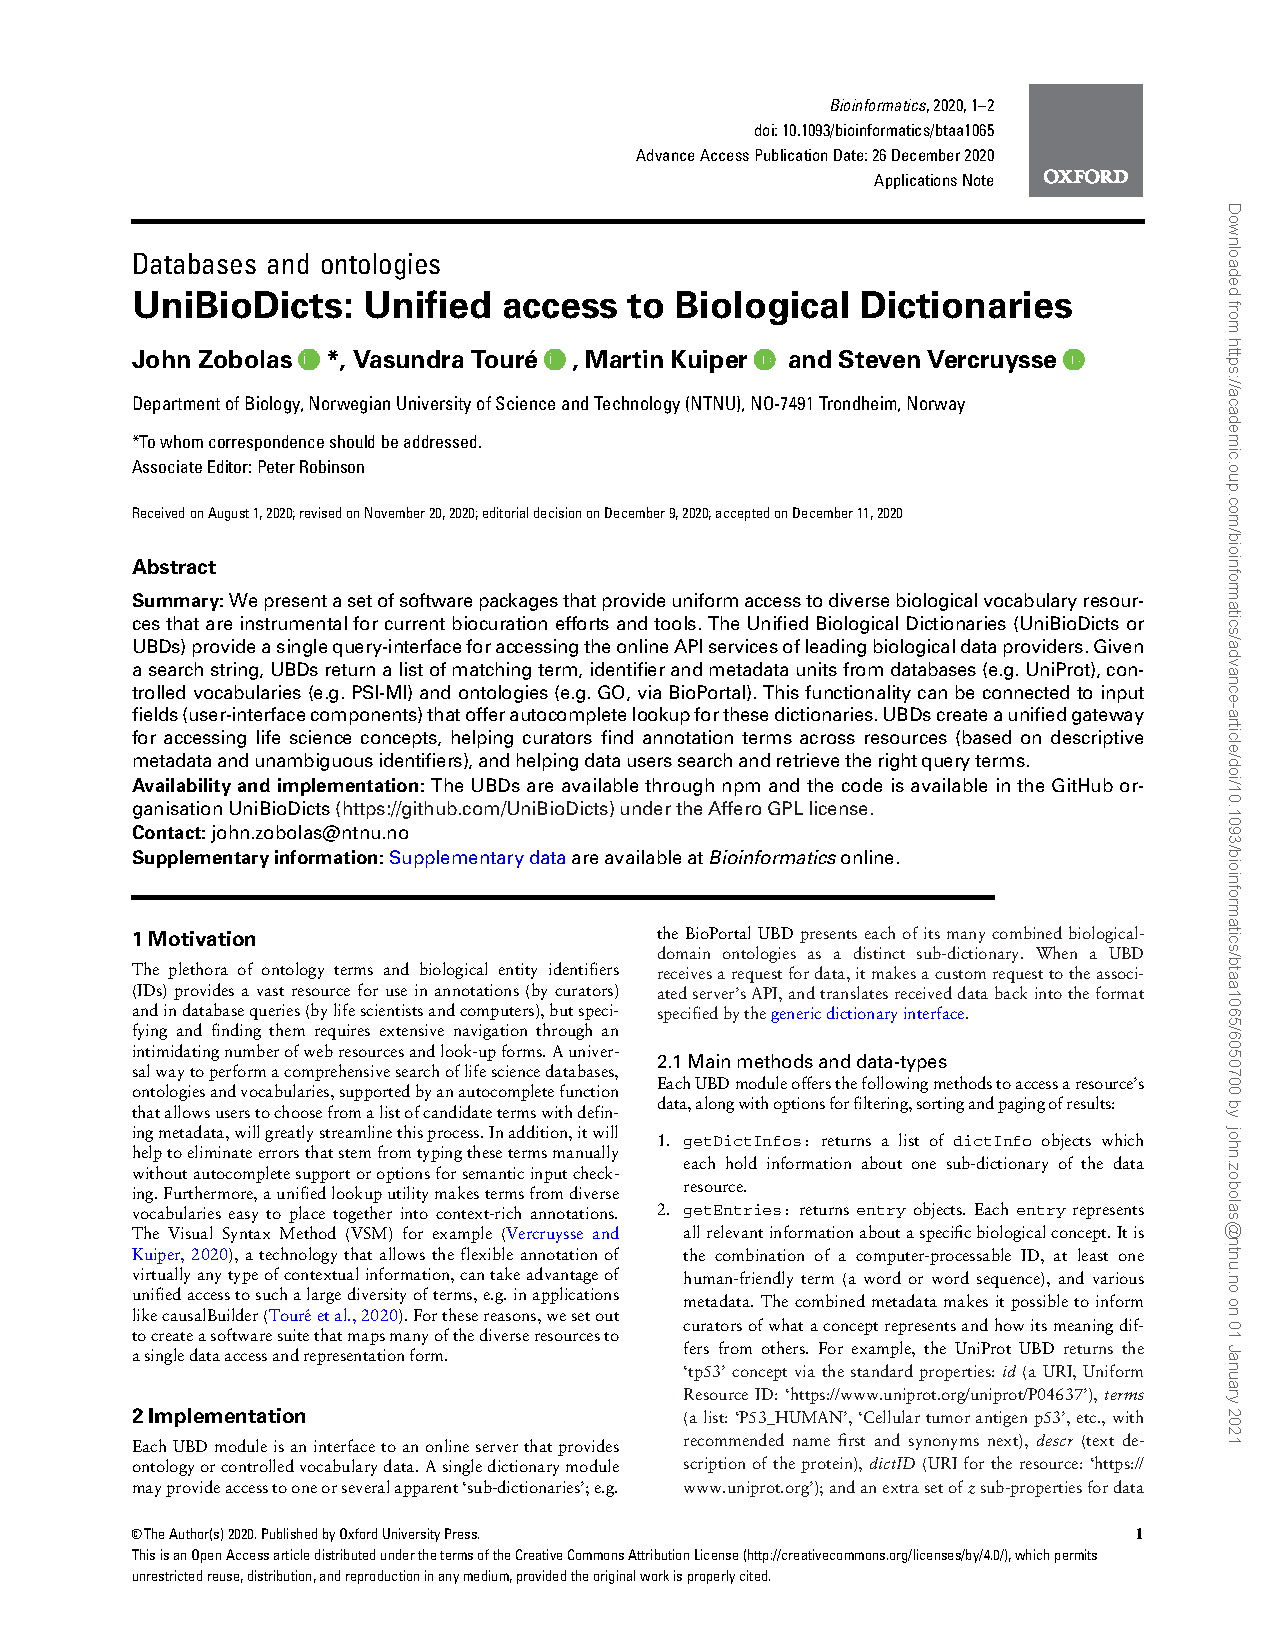
\includepdf[pages=-]{papers/ubds.pdf}

\begin{center}
\vspace*{\stretch{1}}
\textbf{\fontsize{70}{1} \selectfont PAPER 2}
\vspace*{\stretch{1}}
\end{center}

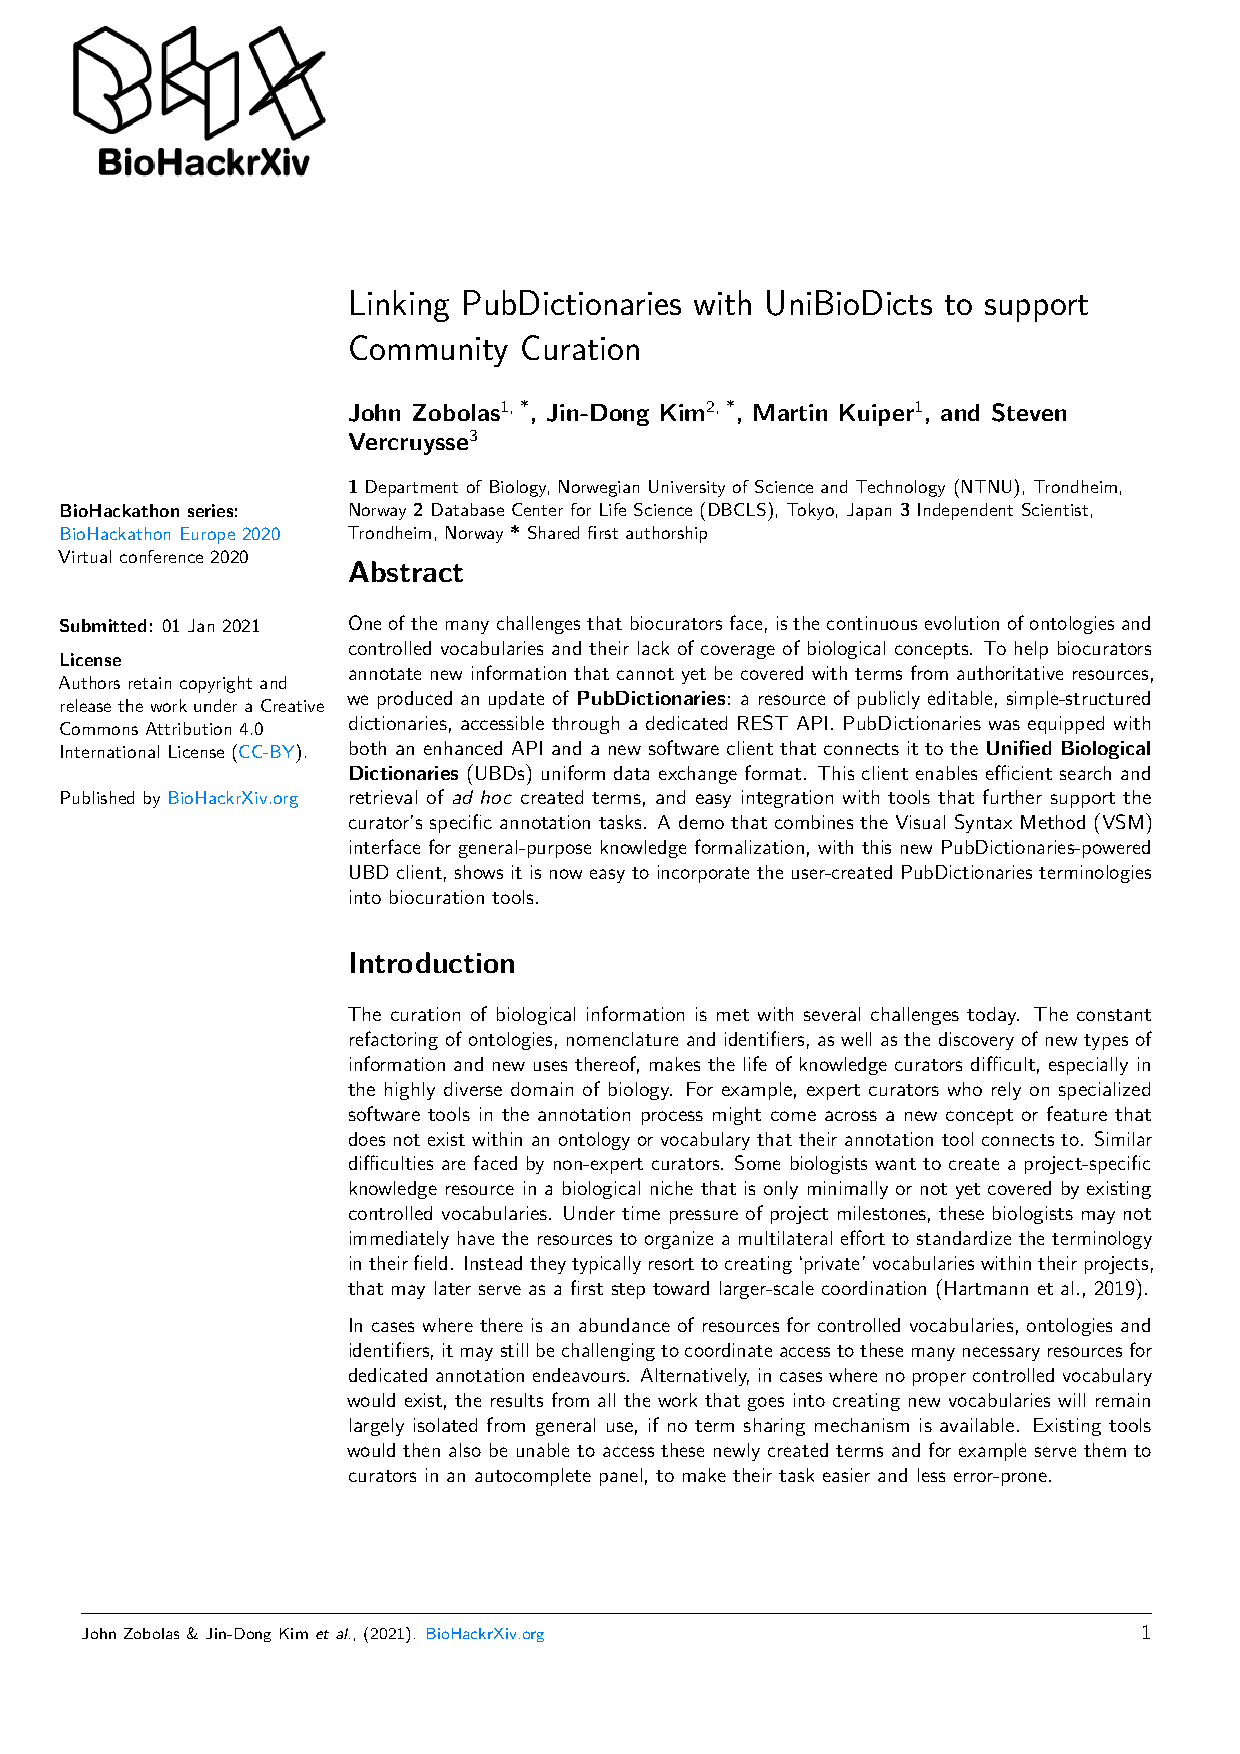
\includepdf[pages=-]{papers/pubdictionaries.pdf}

\begin{center}
\vspace*{\stretch{1}}
\textbf{\fontsize{70}{1} \selectfont PAPER 3}
\vspace*{\stretch{1}}
\end{center}

\includepdf[pages=-]{papers/ags.pdf}

\begin{center}
\vspace*{\stretch{1}}
\textbf{\fontsize{70}{1} \selectfont PAPER 4}
\vspace*{\stretch{1}}
\end{center}

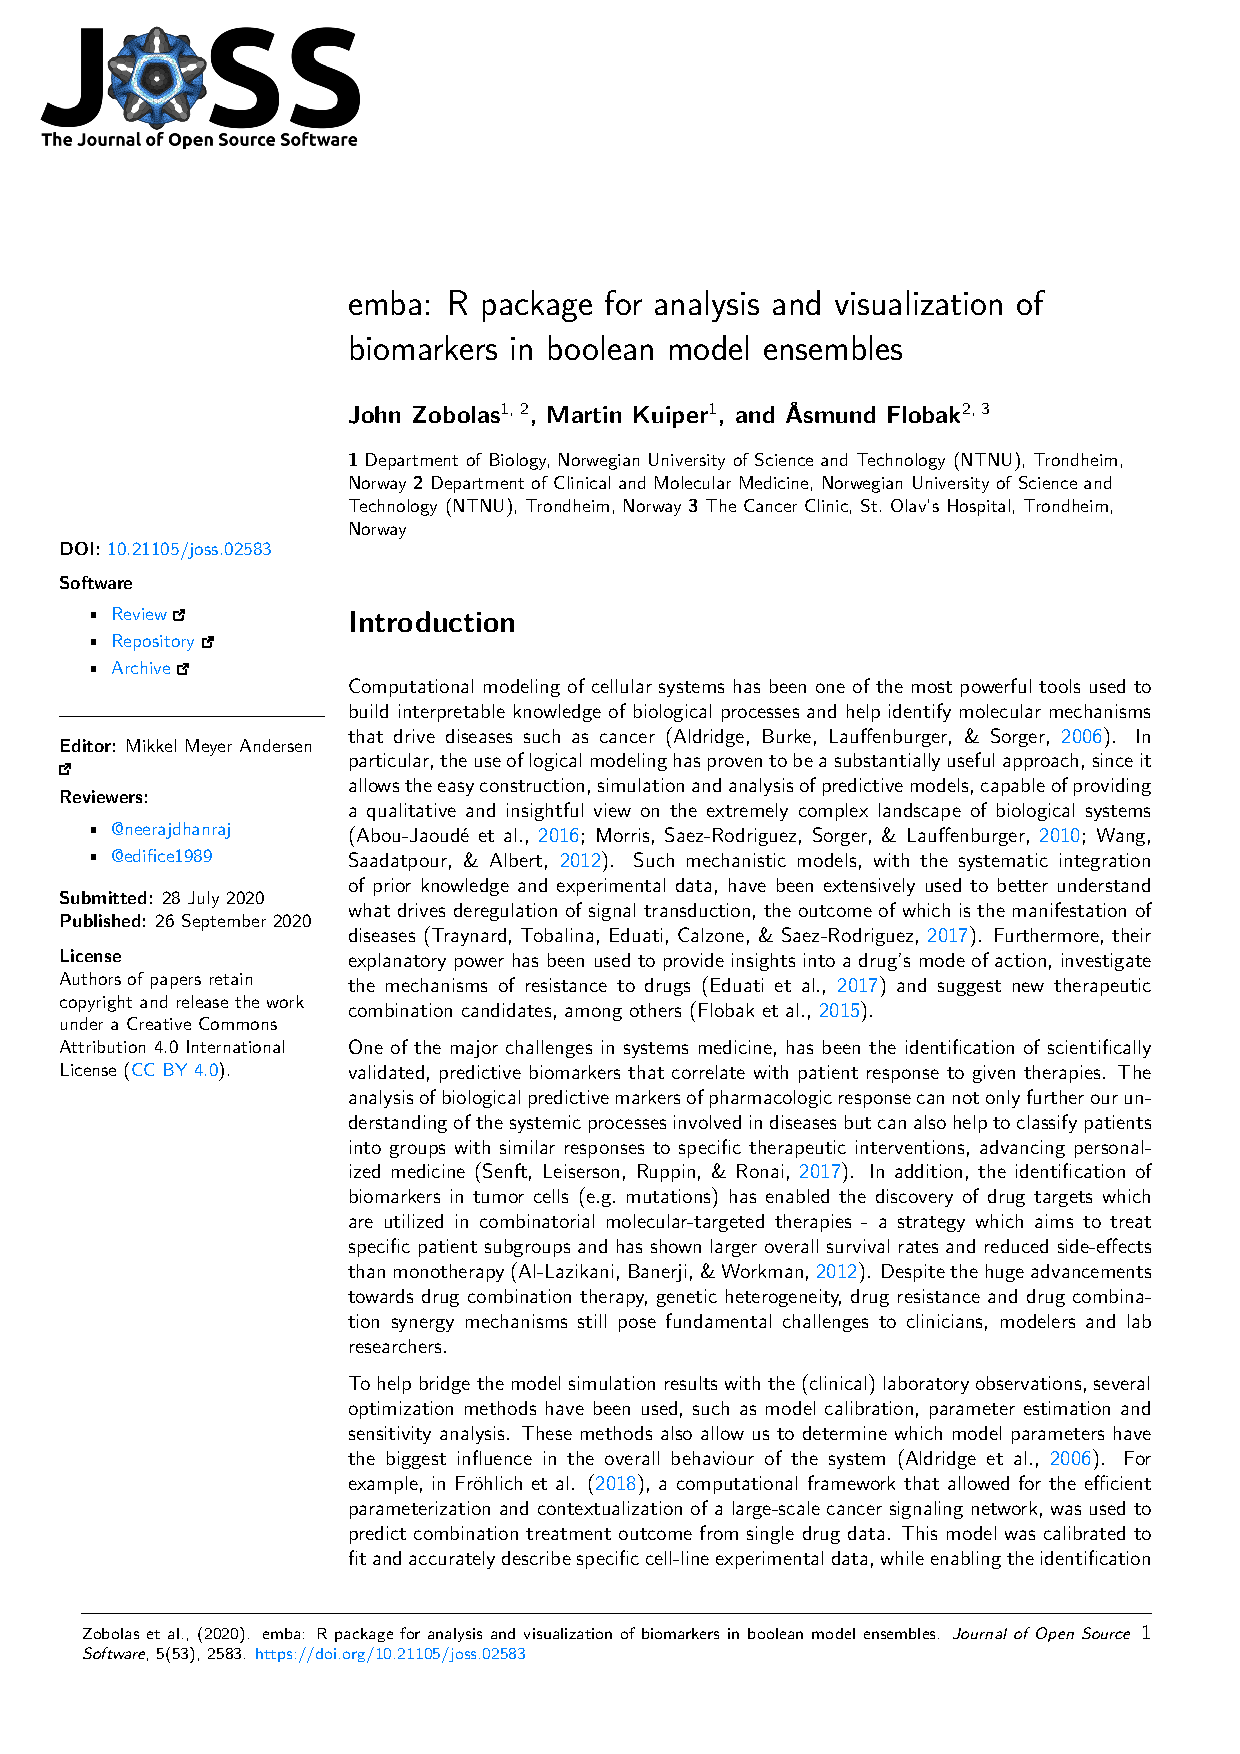
\includepdf[pages=-]{papers/emba.pdf}

\begin{center}
\vspace*{\stretch{1}}
\textbf{\fontsize{70}{1} \selectfont PAPER 5}
\vspace*{\stretch{1}}
\end{center}

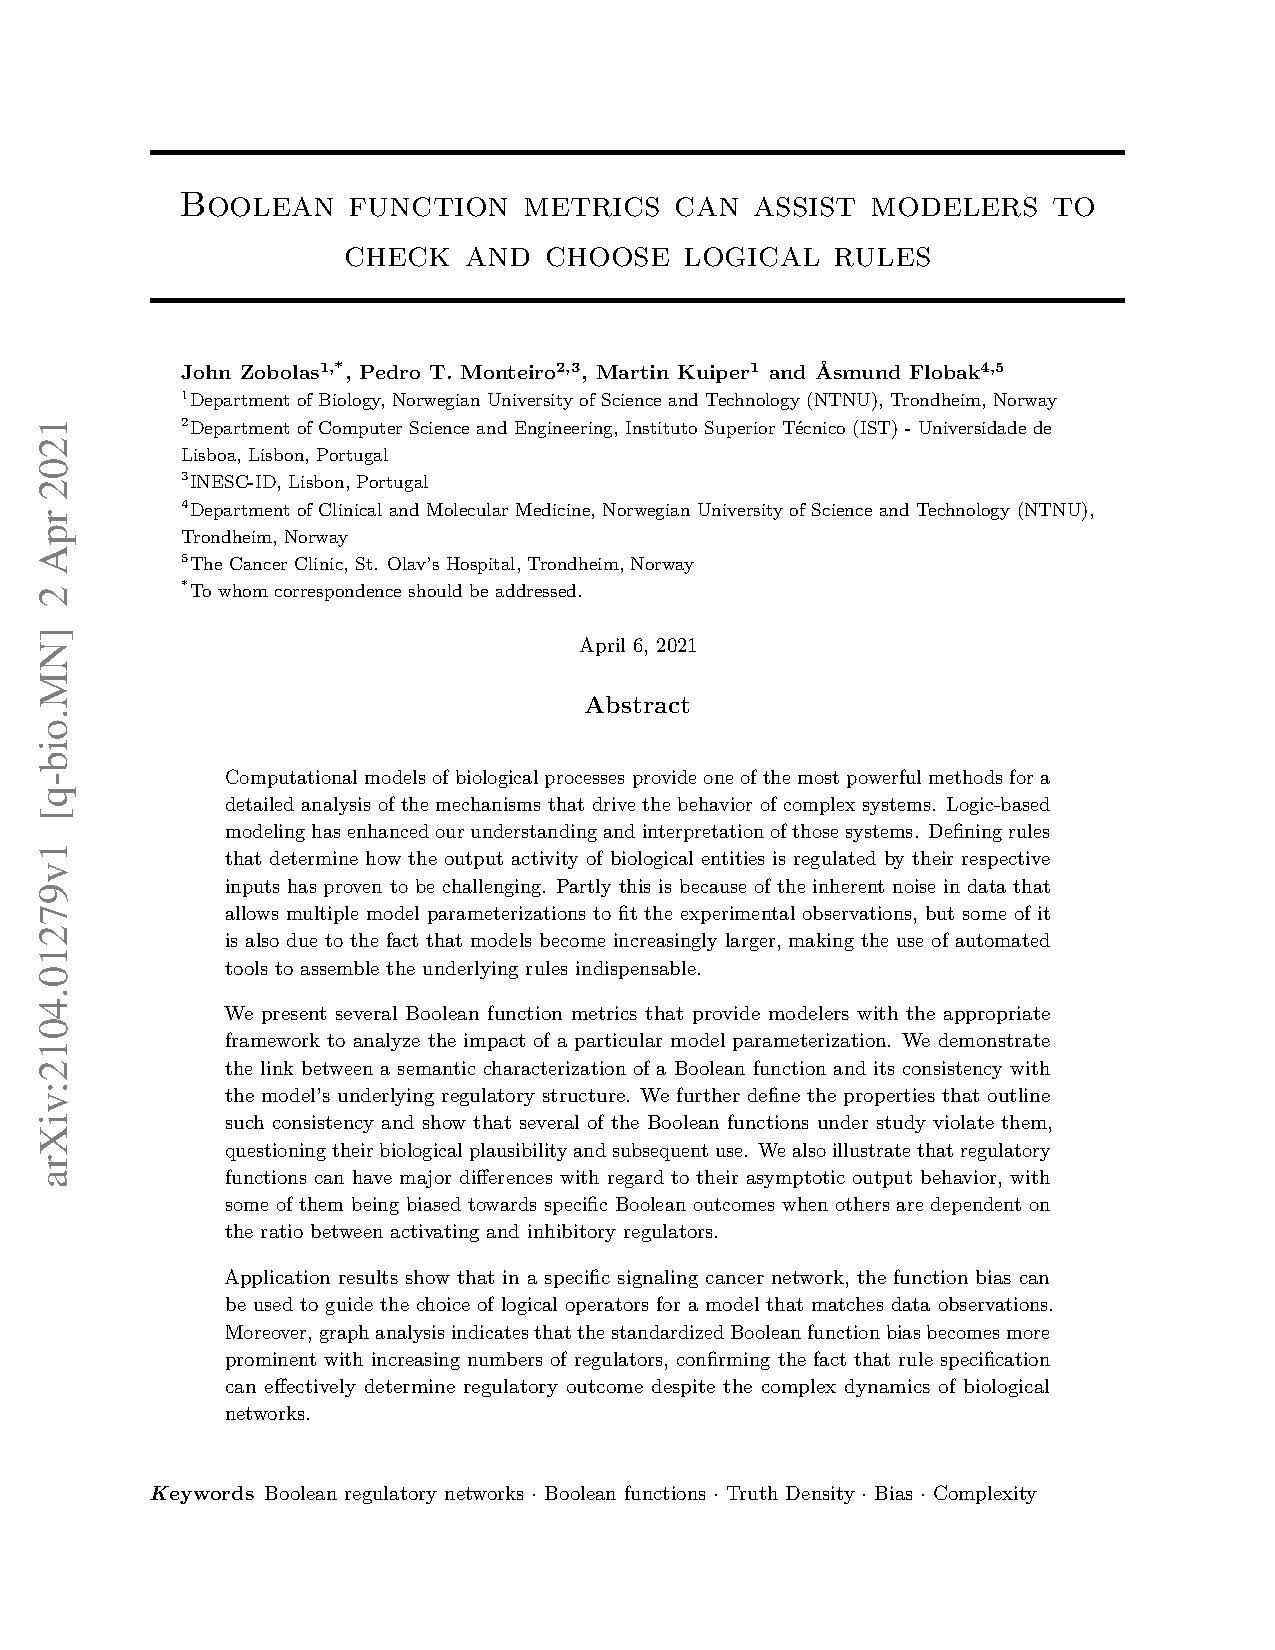
\includepdf[pages=-]{papers/bias.pdf}

\begin{center}
\vspace*{\stretch{1}}
\textbf{\fontsize{70}{1} \selectfont End of Thesis}
\vfill

\includegraphics[width=6cm, height=8cm]{img/rose.jpg}
\vspace*{\stretch{1}}
\end{center}

% list of other candidates at NTNU
%\includepdf[pages=-]{dr_ntnu.pdf}

\end{document}
